%% EXHALE: User Manual
%% Author: Kwang-Il Seon
\documentclass[english,a4paper]{my_memo}
\synctex=1
\usepackage{listings}
\usepackage{xcolor}
\usepackage{booktabs}
\usepackage{longtable}
\usepackage{url}
\urlstyle{tt}
\usepackage{array}
\usepackage{graphicx}
\usepackage{babel}

% listing style for configuration / shell snippets
\definecolor{cfgkey}{rgb}{0.0,0.0,0.55}
\lstdefinestyle{cfg}{
  basicstyle=\ttfamily\small,
  commentstyle=\color{gray}\itshape,
  frame=single,
  breaklines=true,
  columns=fullflexible,
  showstringspaces=false,
}
\lstdefinestyle{sh}{
  basicstyle=\ttfamily\small,
  keywordstyle=\color{cfgkey}\bfseries,
  commentstyle=\color{gray}\itshape,
  frame=single,
  breaklines=true,
}
\newcommand{\rp}{\ensuremath{R_p}}   % \ensuremath, not $R_p$: the bare
                                     % form opened its own math mode and broke
                                     % every use INSIDE math, e.g. $1.67\,\rp$,
                                     % which stopped the whole document building
\newcommand{\msun}{$M_\odot$}
\newcommand{\Rp}{R_{\rm p}}   % planet radius, for use inside math mode

\begin{document}

\title{EXHALE: User Manual}
\author{Kwang-Il Seon}
\date{Last updated: \docmoddate}
\maketitle

\begin{quote}\small\itshape
\textbf{Scope.} This manual describes how to set up, run, and analyze models with
\texttt{EXHALE}, the in-house extension of the ATES (ATmospheric EScape) code
to trace metals, metal-line cooling, a runtime opacity dispatcher, the Roche
tidal potential, and excited-hydrogen / Ly$\alpha$ physics. It documents every
input parameter (with a brief physical meaning), every output file (column by
column, with units), the analysis tools, and a set of worked examples. The
detailed physics derivations live in the companion notes
(\texttt{Update\_EXHALE\_early\_phase.tex}, \texttt{transmission\_spectrum.tex},
\texttt{Update\_EXHALE.tex}, \texttt{cooling\_formulas.tex} (the complete
reference for every analytic cooling coefficient),
\texttt{EXHALE\_BC\_and\_IC.tex} (the boundary- and
initial-condition reference), and \texttt{wind\_ae\_solver.tex}, the
Wind-AE steady-wind solver used by \texttt{IC mode: windae});
this document is the practical user guide.
\end{quote}

\tableofcontents

% ===================================================================== %
\section{Introduction}
% ===================================================================== %

\subsection{What the code does}
\texttt{EXHALE} solves the time-dependent, spherically-symmetric (1-D)
radiation--hydrodynamics of an irradiated planetary upper atmosphere and the
hydrodynamic wind it drives (``atmospheric escape''). It integrates the Euler
equations for mass, momentum, and energy of a single fluid,
\[
\partial_t \rho + \tfrac{1}{r^2}\partial_r(r^2\rho v)=0,\quad
\partial_t(\rho v)+\tfrac{1}{r^2}\partial_r(r^2\rho v^2)+\partial_r p
   = -\rho\,\partial_r\Phi,
\]
\[
\partial_t E + \tfrac{1}{r^2}\partial_r\!\big(r^2 v(E+p)\big)
   = -\rho v\,\partial_r\Phi + \mathcal{H} - \mathcal{C},
\]
to a steady state, where $\Phi$ is the gravitational (optionally Roche) potential
(\S\ref{sec:potential}), $\mathcal{H}$ is the XUV photoionization heating and
$\mathcal{C}$ the radiative cooling. Coupled to the hydrodynamics, at every step it solves the
\emph{ionization equilibrium} of H, He, and the trace metals (C, N, O, Mg, Si,
Ca, Na, K, S, Fe) with a Newton (MINPACK) solver, including photoionization,
collisional ionization, radiative + dielectronic recombination, and charge
exchange. The photoelectron energy budget carries secondary ionization (a fast
photoelectron drives further H\,I / He\,I / H$_2$ ionizations instead of
thermalizing fully) on the Shull \& van Steenberg (1985) ionization budget
with the Dalgarno, Yan \& Liu (1999) heating fraction and molecular channels,
the He\,II\,$\to$\,He\,I
recombination radiation is coupled to H\,I ionization on the spot (Draine 2011
$y$/$z$), and the He\,$\leftrightarrow$\,H charge-exchange pair (Koskinen 2013)
acts in every helium-bearing ionization system. When the metastable He\,$2\,^3$S
triplet is included the code adds its explicit collisional-excitation cooling
(the 10830\,\AA\ channel) and the He\,$2\,^3$S\,$+$\,H / H$_2$ Penning
ionization that removes the metastable. The converged run yields the radial
profiles of density, velocity,
temperature, and the ionization state, plus the steady-state \emph{mass-loss
rate} $\dot M$. A post-processing pass adds advection to the ionization balance,
and the Python tool \texttt{EXHALE\_transit.py} turns a converged model into transit
\emph{transmission spectra} (He\,10830, Ly$\alpha$, H$\alpha$/H$\beta$, and the
metal resonance lines Mg\,II, Ca\,II, Na\,I).

\subsection{The lower boundary, radii, and normalization}
The computational domain starts at a \textbf{lower boundary} placed at the
$1\,\mu$bar pressure level, which defines $r=1$ and the base radius $R_p$ (the
input \texttt{Planet radius}). The base number density $n_0$ and temperature
$T_0$ (the equilibrium temperature) are set there. Internally the code is
non-dimensional: lengths in $R_p$, velocities in $v_0=\sqrt{k_BT_0/\mu}$,
densities in $n_0$, etc. \emph{All output files are written back in cgs} (see
\S\ref{sec:outputs} for the exact normalization of each column). The key
dimensionless number is the \emph{Jeans / escape parameter}
$b_0 = GM_p\mu/(k_BT_0R_p)$, the depth of the gravitational well in units of the
thermal energy; small $b_0$ means an easily-escaping (or tidally unbound)
atmosphere.

\subsection{The gravitational potential}\label{sec:potential}
The potential $\Phi$ in the momentum and energy equations is selected by
\texttt{Domain mode} (Table~\ref{tab:inp-opt}). The code writes it in the
dimensionless units introduced above (lengths in $R_p$, potential in
$v_0^2=k_BT_0/\mu$), so it is fixed by just three numbers: the Jeans parameter
$b_0=GM_p\mu/(k_BT_0R_p)$, the stellar-to-planet mass ratio $q=M_\star/M_p$, and
the orbital separation $\tilde a=a/R_p$.

\paragraph{Spherical mode (\texttt{Domain mode: Spherical}).}
Only the planet's own gravity is kept, so the domain can extend far past the Hill
radius:
\[
\phi(r) = -\frac{b_0}{r}.
\]

\paragraph{Roche mode (default).}
The full co-rotating Roche potential, evaluated along the star--planet
(substellar) line $x=r$, adds the stellar tidal attraction and the centrifugal
term of the synchronously-rotating frame:
\[
\phi(r) = -\frac{b_0}{r}
          \;-\;\frac{b_0\,q}{\tilde a - r}
          \;-\;\frac{b_0\,(1+q)}{2\,\tilde a^{3}}
                \left(\frac{q\,\tilde a}{1+q} - r\right)^{2},
\]
where the second term is the star's gravity at distance $\tilde a-r$ and the
third is the centrifugal potential about the center of mass at
$x_{\rm cm}=q\,\tilde a/(1+q)$ with orbital frequency $\Omega^2=G(M_p+M_\star)/a^3$
(synchronous rotation). The effective gravity used by the hydrodynamics is
$g(r)=-\,\mathrm d\phi/\mathrm dr$, with
\[
\frac{\mathrm d\phi}{\mathrm dr} = \frac{b_0}{r^2}
   - \frac{b_0\,q}{(\tilde a-r)^2}
   + \frac{b_0\,(1+q)}{\tilde a^{3}}\left(\frac{q\,\tilde a}{1+q}-r\right).
\]
The inner Lagrange point $L_1$ is the root of $\mathrm d\phi/\mathrm dr=0$, where
planetary gravity, the stellar tide, and the centrifugal force cancel; in Roche
mode the outer boundary is placed at this $L_1$ radius by default, beyond which
gas is no longer bound to the planet.

\paragraph{Roche mode with an extended outer boundary (\texttt{Outer radius} in
Roche mode).}
By default Roche mode truncates at $L_1$. Supplying an explicit
\texttt{Outer radius [R\_p]:}~$>1$ \emph{without} \texttt{Domain mode: Spherical}
now keeps the full tidal Roche potential above \emph{and} pushes the outer
boundary out to the requested radius (e.g.\ $10\,R_p$), reproducing the
extended-domain treatment of Yan et al.\ (2022) / Huang et al.\ (2023), whose
escape models retain the tidal force but integrate well past $L_1$. This differs
from \texttt{Domain mode: Spherical}, which also extends the domain but
\emph{drops} the tidal and centrifugal terms (pure $-b_0/r$). Two caveats apply.
First, beyond $L_1$ the Roche potential is past its maximum, so the net force is
outward and the 1-D radial flow there is a spherical approximation to what is
physically an $L_1$ funnel: the same approximation Yan/Huang make. Second, the
cold hydrostatic IC is invalid past $L_1$; use \texttt{IC mode: auto} (or
\texttt{transonic}) so the solver seeds a transonic wind through the interior
sonic point. The tidal singularity of the $-b_0\,q/(\tilde a-r)$ term sits at the
star ($r=\tilde a\gg10$), so a $10\,R_p$ domain is numerically safe.

\paragraph{Full 3-D form (transmission post-processing).}
The 3-D Roche-equipotential reconstruction in \texttt{EXHALE\_transit.py} /
\texttt{roche\_recon.py} (\S\ref{sec:tpm}) needs the potential off-axis as well.
With the substellar direction $\hat x$ pointing toward the star and $(y,z)$ the
sky plane,
\[
\phi(x,y,z) = -\frac{b_0}{\sqrt{x^2+y^2+z^2}}
   - \frac{b_0\,q}{\sqrt{(\tilde a-x)^2+y^2+z^2}}
   - \frac{b_0\,(1+q)}{2\,\tilde a^{3}}
        \Big[\big(x_{\rm cm}-x\big)^2 + y^2\Big],
\]
which reduces to the substellar $\phi(r)$ above on the $+x$ axis. The centrifugal
term involves only the rotation-plane coordinates $(x,y)$, not $z$, so surfaces of
constant $\phi$ are triaxial (most extended toward $L_1$, least along the spin
axis $z$).

\subsection{Workflow}
A model run consists of:
\begin{enumerate}\itemsep2pt
\item Prepare \texttt{input.inp} (planet/star parameters, numerics, physics
  switches), by hand or via the GUI; optionally \texttt{metals.inp} (trace
  metal abundances) and \texttt{opacity.inp} (opacity model).
\item Build and run \texttt{./EXHALE.x}; it reads the input files from the current
  directory and writes profiles to \texttt{output/}.
\item Inspect with \texttt{EXHALE\_plots.py} (live profiles) and the example
  notebook; compute transmission spectra with \texttt{EXHALE\_transit.py}.
\end{enumerate}

% ===================================================================== %
\section{Installation and running}
% ===================================================================== %

\subsection{Requirements}
A Fortran compiler (\texttt{gfortran} by default; Intel \texttt{ifort}/\texttt{ifx}
supported), \texttt{make}, and (for the GUI and analysis) Python~3 with
\texttt{tkinter}, \texttt{numpy}, \texttt{scipy}, \texttt{matplotlib}, and
\texttt{astropy} (the last is used by \texttt{EXHALE\_transit.py} for
\texttt{astropy.convolution}).

\subsection{Build}
\texttt{EXHALE} uses an incremental \texttt{Makefile}; module dependencies
are auto-generated, so only edited sources and their dependents recompile.
\begin{lstlisting}[style=sh]
make                 # build ./EXHALE.x with gfortran
make FC=ifort        # Intel ifort   (or FC=ifx for the LLVM compiler)
make wind_ae_ic      # standalone Wind-AE IC generator -> ./wind_ae_ic.x
make check           # byte-identical regression against the stored goldens
make clean           # remove .o/.mod (keeps EXHALE.x)
make distclean       # wipe build/ and EXHALE.x
\end{lstlisting}
\texttt{make check} rebuilds, re-runs each regression case single-threaded
(\texttt{OMP\_NUM\_THREADS=1}, so the result is deterministic) and
\emph{bitwise}-compares \texttt{output/Hydro\_ioniz.txt} and
\texttt{output/Ion\_species.txt} against the stored reference outputs. The
standing rule it encodes: a refactor with no intended physics change must be
byte-identical, and a new physics option must default to off. The harness and
its reference outputs live in \texttt{backup/regression/}; the target reports
that it found no harness, without failing, in a checkout that does not carry
it. \texttt{make wind\_ae\_ic} builds the out-of-process IC generator described
in \S\ref{sec:windae}.

\subsection{Running}
The driver script \texttt{run\_EXHALE.sh} (1) launches a Python/Tk GUI that writes
\texttt{input.inp}, (2) builds, and (3) runs \texttt{./EXHALE.x}:
\begin{lstlisting}[style=sh]
chmod +x run_EXHALE.sh
./run_EXHALE.sh           # gfortran (GUI -> build -> run)
./run_EXHALE.sh --ifort   # Intel ifort   (--ifx for ifx)
\end{lstlisting}
The GUI writes the legacy core block only: it offers \texttt{Load from file},
\texttt{Power-law} and \texttt{Monochromatic} as spectrum types, and every
optional key of Table~\ref{tab:inp-opt} (\texttt{Spectrum type: Planck} and
the two stellar quantities it needs among them) is added to the written file
by hand or inherited by copying an \texttt{examples/} configuration.

You may equally skip the GUI: place a hand-written \texttt{input.inp} (and
optional \texttt{metals.inp}/\texttt{opacity.inp}) in a run directory, ensure an
\texttt{output/} subdirectory exists, and run \texttt{./EXHALE.x} there. Each
modeled planet typically lives in its own subdirectory holding its
\texttt{input.inp}, its \texttt{EXHALE.x}, and its \texttt{output*/} folders.
Progress (iteration counter, the mass-flux spread \texttt{du}, and the
time-derivative norm \texttt{dtu}) is printed to the terminal; the run stops when
\texttt{du} or \texttt{dtu} falls below its convergence threshold.

\subsection{Convergence control}\label{sec:convctl}
The time loop stops when \emph{any} of the following criteria is met
(defaults in \texttt{src/modules/init/parameters.f90}; most are runtime-settable,
Table~\ref{tab:inp-opt}):
\begin{center}\small
\begin{tabular}{@{}lll@{}}
\toprule
Parameter & Default & Stop condition \\
\midrule
\texttt{du\_th}    & $1\times10^{-3}$ & mass-flux spread $du<\texttt{du\_th}$ \\
\texttt{dtu\_th}   & $1\times10^{-8}$ & time-derivative $\infty$-norm $dtu<\texttt{dtu\_th}$ \\
\texttt{stall\_tol}, \texttt{N\_stall} & $10^{-6}$, 2000 & $du$ on a plateau for \texttt{N\_stall} steps \\
\texttt{count\_max} (\texttt{Max steps:}) & $10^{6}$ & hard iteration cap \\
\bottomrule
\end{tabular}
\end{center}
\noindent
$du$ is the radial spread of the mass flux $F=\rho v r^2$ over the convergence
window $r\ge$ \texttt{Escape radius} (cells $j_{\min}\ldots N$),
\[
  du = \frac{\max_j F_j - \min_j F_j}{|\,\overline{F}\,|},
  \qquad \overline{F}=\frac{1}{N-j_{\min}+1}\sum_{j=j_{\min}}^{N} F_j ,
\]
with $F$ taken \emph{signed}: no absolute value is applied before the extrema,
so a window whose flux reverses (inflow at one radius and outflow at another)
is measured as the far-from-steady state it is rather than read as flat, and
the normalization is the window's own mean level, floored at $10^{-30}$ so that
a vanishing mean gives a large number rather than an infinity. A steady
spherical wind carries one mass flux at every radius, which is what this
measures. It is evaluated once per step by a single function
(\texttt{mass\_flux\_spread} in \texttt{EXHALE\_main.f90}) that the $du$ stop,
the arming of the $du$ triggers, the PLM\,$\to$\,WENO3 stage flip, the
secondary-ionization flip and the JFNK hand-off all read, so every one of them
speaks about the same number; the value at the final step is written to
\texttt{run.log}. It is \emph{not} a velocity change or a step-to-step
variation: that is \texttt{dtu}.

The stall and \texttt{count\_max} backstops guarantee termination even when the
strict $du$/$dtu$ thresholds are physically unreachable for a given setup (e.g.\ a
transonic wind whose $du$ floors at $\sim1\%$). Each iteration prints
\texttt{count, du, dtu} (and the windowed flux-level change when
\texttt{Level tol:} is set), and the run reports which criterion stopped it. The
optional \texttt{Force start} forces the first 1000 iterations regardless (useful
when starting near a fixed point).

Two of these triggers are \emph{armed} before they can fire. A generated
initial condition (cold hydrostatic, transonic, warm-seed, Wind-AE) is an
analytic profile the marching loop has not touched, so its $du$ measures the
smoothness of the formula that built it, not relaxation of the wind, and it can
start orders of magnitude below every threshold. The $du<\texttt{du\_th}$ stop
and the Newton hand-off (together with the secondary-ionization flip that shares
its $du$ comparison) therefore require $du$ to have been seen at or above their
own threshold first, so only a \emph{descending} crossing stops the run; both
arm immediately when the run started from \texttt{Load IC?\ True}, whose state
was relaxed by the run that wrote it. Arming is reported in the log. The
PLM\,$\to$\,WENO3 switch is deliberately not guarded. The rationale and history of these settings are
in \texttt{Update\_EXHALE\_solver}.

\paragraph{Caveat: $du$ can stop a run prematurely.} $du$ measures only the
\emph{spatial spread} of $\rho v r^2$ in the wind window; it is blind to a
uniform drift of the flux level (the mean it normalizes by drifts with it), and on strongly irradiated planets it
\emph{oscillates}, dipping below $10^{-3}$ transiently long before the wind
settles. A WASP-121b reference stopped this way was low by $\sim$0.08 dex in
$\dot M$ with the heating/cooling grossly out of balance (energy residual
$\sim$30). For production answers use the residual-based stop
(\texttt{Resid tol:}) or the Newton finish (\texttt{Solver: Newton},
\S\ref{sec:newton}); details in \texttt{steady\_solver\_memo}.

\paragraph{Staged secondary ionization.} With
\texttt{Secondary\_ionization: True} (the default) the photoelectron coupling
is \emph{not} applied from step~0. From a cold initial condition
it would deepen the base cooling valley and amplify the base acoustic mode into
a NaN runaway on high-gravity cases. Instead the wind first relaxes without the
coupling; the moment that first relaxation converges (or stalls) the coupling
switches on (the terminal prints \texttt{secondary ionization activated at step
N}), the convergence logicals and flux-level history are reset, and stops are
held for \texttt{N\_stall} steps while the base adjustment wave forms, after
which the run re-converges with the full physics. Expect roughly double the step
count on high-gravity cases. \texttt{Secondary\_ionization: False} disables the
coupling entirely; \texttt{Immediate} applies it from step~0 (for A/B tests
only: it reproduces the cold-start crash on high-gravity cases).

\textbf{A consequence worth knowing before reading a short run.} Staged is not
a synonym for on. A run that never reaches its first convergence (one
stopped at a fixed step count, or one left at a du plateau) never switches
the coupling on, and its answer carries no secondary ionization at all. The
startup report (\texttt{EXHALE\_setup.out}) says which of the three states the
run is in, and the terminal prints the activation line only when it happens.

\subsection{Base grid resolution (\texttt{Base grid [dr,cells]})}
\label{sec:basegrid}
The \texttt{Mixed} grid stacks \texttt{cells} uniform cells of size \texttt{dr}
(in \rp) on the lower boundary and fills the rest of the domain with
$N-\texttt{cells}$ geometrically stretched cells; the total cell count $N$ is
set by the optional key \texttt{Grid cells:} (default 500). The two numbers
share one input line because they are not independent: their product is the
radial extent of the uniform region ($0.01\,R_p$ with the default
\texttt{2.0e-4 50}).

The quantity that matters physically is how many uniform cells span the base
density scale height, $H/dr$ with $H=kT/(\mu g)$. Where $H/dr$ is of order a few
cells the discretization supports a \emph{stationary} $2\,dr$ entropy (contact)
mode that nothing in the scheme removes: HLLC resolves a contact of zero speed
exactly and so adds no dissipation to it, the gravity source is cell-local, the
WENO3 pressure gradient sees only interface pressures, and there is no
conduction or physical viscosity unless they are switched on. The measured
dependence is an alternating $\ln\rho$ amplitude of $\sim$$10^{-2}$ for
$H/dr<5$ and $\sim$$10^{-4}$ for $H/dr>100$. High-gravity planets have the
least margin: at $T_{\rm eq}$ on the default grid HD\,189733\,b spans only
$\sim$27 cells per $H$, against $\sim$60--100 for HD\,209458\,b, WASP-52\,b and
WASP-121\,b, and a cool, shielded base shrinks $H$ further. The value in
effect is echoed in \texttt{EXHALE\_setup.out} as \path{Base scale-height
resolution: H(T_eq)/dr}, with a warning below 10 cells.

Refine at fixed extent, i.e.\ divide \texttt{dr} and multiply \texttt{cells} by
the same factor: \texttt{Base grid [dr,cells]: 5.0e-5 200} is the $4\times$
refinement. Two costs follow. The CFL time step is set by the smallest cell, so
a $4\times$ finer base means $\sim$$4\times$ more steps for the same physical
time; and at fixed $N$ the stretched region loses those cells and coarsens
(for a $4.43\,R_p$ domain, the cell size at $1.5\,R_p$ grows from
$6.1\times10^{-3}$ to $1.3\times10^{-2}\,R_p$). Raising \texttt{Grid cells:}
alongside the refinement keeps the upper stretch fixed instead: the pairs
\texttt{1.0e-4 100}/500, \texttt{5.0e-5 200}/658, \texttt{2.5e-5 400}/916 and
\texttt{1.25e-5 800}/1375 hold the stretch ratio at its default-grid value,
at the price of proportionally more work in every sweep. In practice the
$2\times$ step
(\texttt{1.0e-4 100}) is the one to try first: it is where the mode goes, and
$4\times$ is not reachable to convergence on HD\,189733\,b within the
step cap (\texttt{Max steps:}) because its time step is $4\times$ smaller.

\paragraph{The exact default width, and inputs written before it was pinned.}
The default \texttt{dr} is the double $2.0\times10^{-4}$ written in the
source with a \texttt{d} exponent, so the value is the one a reader of the
key would spell: an \texttt{input.inp} without the key and one stating
\texttt{Base grid [dr,cells]: 2.0e-4 50} build the same grid to the bit, the
list-directed read of \texttt{2.0e-4} into a \texttt{real*8} being that
double.  This matters because the grid is part of a stored state: a restart
is refused when the file's cell centers differ from the run's by more than
$10^{-10}$ relative.  An input written before 2026-09-19 was run on the
default-real literal, the width $1.9999999494757503\times10^{-4}$, whose
centers differ from the present grid's by $3.8\times10^{-9}$ to
$6.6\times10^{-9}$ relative, which exceeds that tolerance.  Every such input
standing beside stored results carries that width explicitly as
\texttt{Base grid [dr,cells]: 1.9999999494757503e-4 50}
(\texttt{src/utils/pin\_base\_grid.py}), and each preserved tree whose
inputs were not edited has a \texttt{GRID\_DEFAULT\_NOTE.md} at its root
stating the same line.  The width a run used is recorded at round-trip
precision in the resolved-configuration record, and the refusal itself prints
it with where it came from, the key or the default. That $2\times$
setting is what \texttt{HD189733b/input.inp} carries; the other three production
planets run on the default. The full investigation is
\texttt{docs/hd189\_base\_checkerboard.md}.

\subsection{The lower boundary: a characteristic condition at the face}
\label{sec:basebc}
The lower boundary is imposed at the first cell \emph{face} $r_{\rm edg}(0)$,
not in a ghost cell. At that face the characteristic speeds are $v-c$, $v$ and
$v+c$, and a wave enters the domain when its speed is positive; in EXHALE the
radius increases outward, so gas entering the base moves outward and inflow is
$v>0$. For the subsonic inflow a wind rests on, two characteristics enter and
one leaves, so the lower atmosphere states \emph{two} conditions and the
interior supplies \emph{one}.

The two the lower atmosphere states are its \textbf{pressure} and its
\textbf{specific entropy} at the base level $r=1$, carried as the isentrope
through $(p_0, T_0)$ at the base composition. The one the interior supplies is
the outgoing acoustic invariant of the first cell,
\begin{equation}
  p_b - \rho_i c_i\, v_b \;=\; p_i - \rho_i c_i\, v_i ,
\end{equation}
where the subscript $i$ is cell~1 continued to the face along its own
hydrostatic isentrope and $c_i$ uses cell~1's own $\gamma_{\rm eff}$. The
closed-form invariant $v-2c/(\gamma-1)$ is deliberately not used: the caloric
equation of state gives every cell its own $\gamma_{\rm eff}(x_{\rm H_2},T)$,
and that invariant assumes one constant $\gamma$.

The ghost cells are then the volume averages of the same hydrostatic isentrope
continued \emph{below} the face, with the velocity carrying a constant
$\rho v r^2$. They are not copies of the face state: the two differ by half a
cell of stratification, and that half cell is what the previous ghost-cell
closure left as a resolution-independent momentum imbalance of $25\%$ of the
weight of cell~1.

Where the flow reverses ($-c<v<0$) only one characteristic enters, so the
reservoir states the pressure alone and the entropy at the face is the
interior's, advected out. That choice is discrete and has no width: a contact
carrying different entropies on its two sides has direction-dependent traces,
and a face density between them is an interpolation rather than a law of
thermal contact. The side that owns the face is the side the level's mass flux
comes from, read from the wind window $r\ge r_{\rm flux}$ where that window
carries one flux (its relative standard deviation at or below
$2\times10^{-3}$ and its face-mapped Mach number at or above $10^{-12}$), and
from the matched face velocity where it does not, a velocity below the
rounding of the cancellation it is formed from counting as zero. At rest and
at inflow the reservoir owns the level, the physical assumption being that the
lower atmosphere below it is a radiatively controlled heat bath. Supersonic
outflow prescribes nothing, and that transition alone carries a declared
numerical width, a smoothstep of half width $10^{-8}$ in $M_i$ about $-1$,
where the number of outgoing characteristics changes. Supersonic \emph{inflow}
would need three reservoir conditions and a $(p,s)$ reservoir has two, so it is
reported as a configuration outside the model rather than repaired.

The composition of the two lower ghost cells is part of the boundary model as
well, and is what distinguishes model v3 from v2 in the state file's
\texttt{\# boundary\_model} line. The ghost composition is not prescribed but
solved by the ionization sweep, and the sweep is a map from the composition it
is entered at to the one it returns, so under v2 two entry compositions could
return ghosts $4.7\times10^{-3}$ to $5.5\times10^{-2}$ apart in their trace
ions, both accepted by every test the sweep applies, and the base continuity
row of cell~1 read $8.335\times10^{-8}$ in one and $2.923\times10^{-9}$ in
the other against the same tolerance. v3 states both halves of the fix: the
ghost solve starts from the reservoir row at the first sweep and from the
ghost the previous sweep returned after it, and the ghost it returns is held
to a fixed point of that same map, the largest absolute change of any ghost
species density in the cell's own units at most $10^{-11}$ and the ghost's
heavy-particle plus electron count moving by at most $10^{-6}$ of itself. A
boundary that cannot reach that in twenty applications stops the run by name
with both moves. Nothing here is a key: the seed and what the fixed point
reached are printed in the boundary report, and the diagnostics that replace
the seed for a measurement are the \texttt{EXHALE\_GHOST\_*} variables of
Table~\ref{tab:env}, all default off.

Nothing in this is selectable. There is no ghost velocity, pressure or
temperature closure to choose, and the four keys that used to choose them
(\texttt{Valve eps}, \texttt{Hydrostatic base}, \texttt{Base ghost
temperature}, \texttt{Base velocity}) are refused at startup with a message
naming the replacement, rather than ignored. The one key that remains is
\texttt{Base BC:}, which states \emph{where} the boundary is, not what it does.

\subsection{The steady-state Newton solver (\texttt{Solver: Newton})}
\label{sec:newton}
The finite-volume steady state can be solved directly ($F(Y)=0$ for the hydro
state, with the ionization equilibrium eliminated locally inside the residual)
by a preconditioned Jacobian-free Newton--Krylov method (banded LAPACK
preconditioner, frozen WENO weights, diagonal scaling, non-monotone line search;
the boundary's one branch of nonzero width, the supersonic-outflow transition,
sits decades from any operating point, so nothing has to be smoothed for it). Each
unknown is scaled by its own cell's state ($\rho$, $\rho(|v|+c_s)$, $E$),
so that no cell sets another's scale; the momentum scale uses the fastest
signal speed because $\rho v$ itself vanishes wherever the flow reverses. This
reaches residual levels unattainable by marching at a small fraction of the cost:
WASP-121b converges in 8 Newton iterations ($\sim$200 marching-steps of cost,
vs.\ $>$35{,}000 insufficient marching steps), HD189733b in 33\,s where marching
spent $>$3\,h without converging.

Two ways to use it:
\begin{itemize}
\item \textbf{Production}: add \texttt{Solver: Newton} to \texttt{input.inp}. The
  run marches (including the two-stage PLM$\to$WENO3 when
  \texttt{Reconstruction scheme: PLM+WENO3} is set) until the flux
  metric $du$ (the radial spread of $\rho v r^2$) drops below the hand-off
  threshold \texttt{newton\_du\_switch} (default $10^{-2}$; the $du$-based
  \emph{convergence} stops are suspended), then the Newton solve finishes to
  \texttt{Resid tol} (default $10^{-5}$), and the standard outputs and
  post-processing follow. The hand-off point is adjustable through an optional
  third token on the key, \texttt{Solver: Newton <du\_switch>} (e.g.\
  \texttt{Solver: Newton 5e-3} hands off later); a bare \texttt{Solver: Newton}
  keeps the $10^{-2}$ default.
\item \textbf{From an existing state} (recommended for re-converging old runs):
  put the state in \texttt{output/*\_IC.txt}, set \texttt{Load IC?\ True} and
  \texttt{Resid tol:\ 1.0e-5}, and run with the environment hook
\begin{lstlisting}[style=sh]
EXHALE_PTC=1 EXHALE_PTC_JFNK=1 EXHALE_PTC_DTAU0=1.0 ./EXHALE.x
\end{lstlisting}
  which solves from the loaded state, writes \texttt{output/}, and stops.
\end{itemize}
The warm start matters: Newton has a finite basin, so the hand-off must wait
until the marching warm-up has flattened the wind. The default
$du<10^{-2}$ is calibrated to land inside the basin: handing off earlier (a
larger \texttt{newton\_du\_switch}) risks starting Newton outside it and
stalling, whereas a cold-IC start (no warm-up at all) stalls outright. Earlier
revisions keyed the hand-off on the residual itself ($\|R\|<5\times10^{-2}$);
the $du$-based key is equivalent in practice and consistent with the flux-based
convergence decision (\S\ref{sec:convctl}), while the residual remains the
\emph{target} of the JFNK finish. Convergence is linear (frozen-weight refresh
and the chemistry noise floor). Planets with a breathing base (HD189733b) used
to stop at a practical floor $\|R\|\sim3\times10^{-4}$; the 2026-08-11
line-search and base-energy fixes removed it, and a warm re-convergence of
HD189733b now reaches $\|R\|=1.2\times10^{-5}$ in 11 outer iterations
(re-measured 2026-08-15).
The Newton finish is also \emph{safe to fail}: the solver tracks the best
iterate seen, aborts once the line search has failed to find any acceptable
step in 12 consecutive outer iterations, and on failure the run prints
\texttt{JFNK failed}, keeps the best
iterate, and falls back to plain time-marching with the $du$-based stops
re-armed: an unconverged Newton state is never accepted as the final
answer. The associated diagnostic hooks (\texttt{EXHALE\_RESIDUAL},
\texttt{EXHALE\_JAC\_TEST}, \texttt{EXHALE\_NEWTON\_TEST}, \ldots) are environment
variables, collected in \S\ref{sec:envvars} (Table~\ref{tab:env}). Full
development record and validation: \texttt{steady\_solver\_memo.pdf}.
Figure~\ref{fig:newton} shows the whole route end-to-end on WASP-121b
(Roche): the monitored residual during the marching warm-up (left; note that the
$du$-based stop would have fired long before the residual is actually small) and
the JFNK finish (right).

\paragraph{What certifies a converged state, and what the exit status says.}
Reaching \texttt{Resid tol} is not the same as being certified. At the
marching stop, at the JFNK final and at a pseudo-transient declaration, one
evaluator builds an inventory of every balance the configuration activates
and returns, for each, a status (\texttt{not\_applicable} /
\texttt{evaluated} / \texttt{unavailable}), the row measure (the maximum over
physical cells of $|{\rm res}|/\max({\rm scale},{\rm floor})$), the volume
average, the worst cell and the scale it was divided by. The tolerances are
$3\times10^{-12}$ for the mass row, $10^{-8}$ for momentum and $10^{-6}$ for
energy, the level balances and the eliminated-species closures.

\emph{The species rows are gated by regime.} An element row and a carrier row
are judged against $10^{-5}$ for cells at $r \ge 1.20\,R_{\rm p}$ only; below
that radius the row is measured and printed and does \emph{not} gate. The
gate is anchored on the element operator's own stated floor and sits a decade
above the discretization error a smooth manufactured column shows at the
production spacing ($1.5\times10^{-6}$); the layer is excluded because its
element fluxes are not conserved there at all (their radial spread over
$r < 1.10$ is $9.8$ times the median), so no threshold means anything against
them yet. The band $1.10 \le r < 1.20$ is likewise reported and does not
gate. A state that passes with species rows present reports that it is
certified \emph{in the wind}, and its state file records
\texttt{cert\_reason=certified\_in\_wind}. The two radii are properties of
the flow and are constants of \texttt{certification.f90}, not input keys; the
five measurements behind the number are in
\texttt{docs/certification\_tolerance\_anchoring\_20260910.md}.

A run that DECLARED a stationary state and then failed certification exits
with status~2; a run that ended on a cap makes no such claim, writes
\texttt{certified=F cert\_reason=no\_stationary\_claim} in its state files and
exits~0. The regression harness never tests the status.

\begin{figure}[htbp]\centering
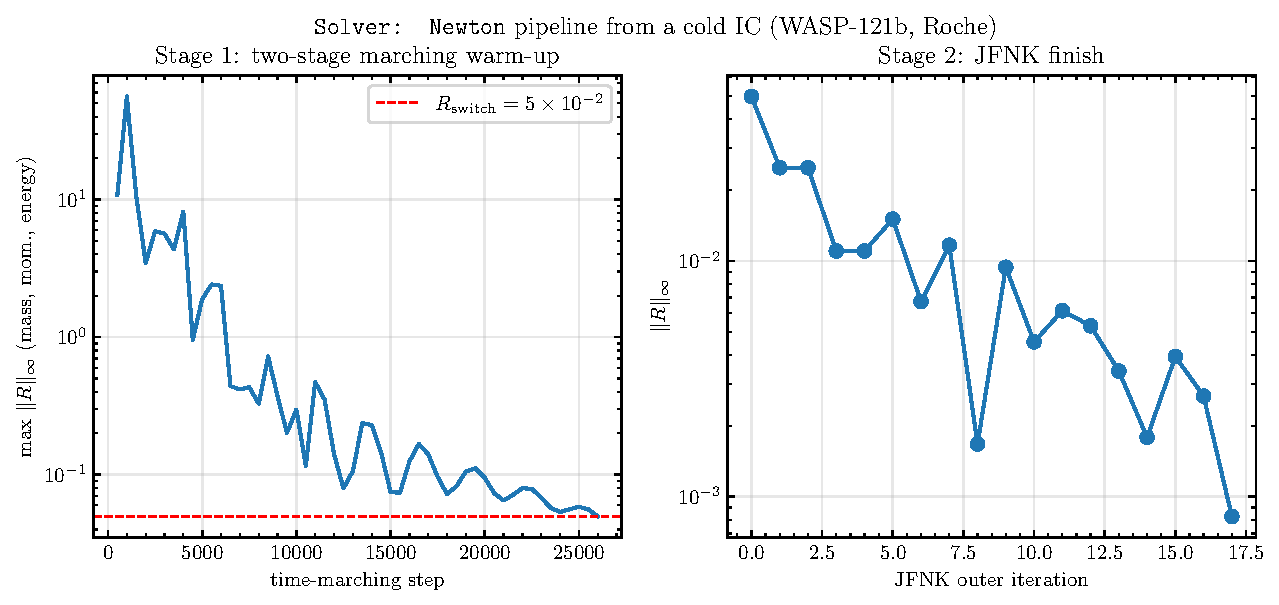
\includegraphics[width=0.95\textwidth]{figures/newton_convergence.pdf}
\caption{The \texttt{Solver: Newton} route from a cold IC (WASP-121b, Roche).
Left: maximum steady residual $\max\|R\|_\infty$ over the mass, momentum, and
energy equations during the two-stage (\texttt{Reconstruction scheme:
PLM+WENO3}) marching warm-up; the dashed line is the
legacy residual hand-off threshold $R_{\rm switch}=5\times10^{-2}$ used when this
figure was produced (the current default keys the hand-off on $du<10^{-2}$
instead, at a comparable point on the warm-up). Right: residual vs.\ JFNK outer
iteration during the Newton finish, down to \texttt{Resid tol} ($10^{-5}$).}
\label{fig:newton}
\end{figure}

\subsection{Environment-variable hooks (diagnostics and expert runs)}
\label{sec:envvars}
A small set of \emph{environment variables} expose diagnostic and expert
entry points without touching \texttt{input.inp} (Table~\ref{tab:env}). They
are read once at startup; when unset they have strictly zero effect, so normal
runs are unaffected. All of them are diagnostics or validation aids, apart from
\texttt{EXHALE\_ROOT}, which the lower-atmosphere pre-step needs: the only
other one used in a production workflow is the \texttt{EXHALE\_PTC} family, which
implements the ``Newton from an existing state'' recipe of \S\ref{sec:newton}
(and \texttt{examples/04\_newton\_from\_state/}). Typical usage:
\begin{lstlisting}[style=sh]
EXHALE_RESIDUAL=1 ./EXHALE.x                      # rank a "converged" state
EXHALE_PTC=1 EXHALE_PTC_JFNK=1 EXHALE_PTC_DTAU0=1.0 ./EXHALE.x   # re-converge it
\end{lstlisting}

{\small
\begin{longtable}{@{}lp{10.2cm}@{}}
\caption{Environment-variable hooks. All are read once at startup and have
zero effect when unset. The four diagnostic tests (top block),
\texttt{EXHALE\_PARSE\_DUMP} and \texttt{EXHALE\_PTC} runs stop after
printing/writing; they do not march.}
\label{tab:env}\\
\toprule
Variable & Effect \\
\midrule
\endfirsthead
\toprule
Variable & Effect \\
\midrule
\endhead
\midrule
\multicolumn{2}{r}{\emph{continued on the next page}}\\
\endfoot
\bottomrule
\endlastfoot
\texttt{EXHALE\_DUMP\_IC=1} & After \texttt{Load IC?\ True}, write the restored
  state to \texttt{output/Hydro\_ioniz.txt} and
  \texttt{output/Ion\_species.txt} and stop, \emph{before} the first
  ionization-equilibrium solve re-equilibrates the species fractions
  (verifies a snapshot/restart round-trip). \\
\texttt{EXHALE\_RESIDUAL=1} & Evaluate the steady residual $R$ of the loaded
  state (WENO3, boundary conditions applied first), print the norms
  for each equation (mass, momentum, energy), and stop. The criterion-independent way to
  rank candidate ``converged'' states (a premature-dip state shows
  $\|R\|_E\sim O(10)$ despite $du<10^{-3}$). \\
\texttt{EXHALE\_NEWTON\_TEST=1} & Self-test of the Newton infrastructure
  (\texttt{pack\_U}/\texttt{unpack\_U} round-trip and the frozen residual
  against the \texttt{EXHALE\_RESIDUAL} values); prints and stops. \\
\texttt{EXHALE\_JAC\_TEST=1} & Verify the colored-FD banded Jacobian against a
  directional finite difference $J\,r\simeq[F(Y+\epsilon r)-F(Y)]/\epsilon$;
  a correct band layout matches to $\sim10^{-6}$, a wrong one is $O(1)$ off.
  Prints and stops. \\
\midrule
\texttt{EXHALE\_PTC=1} & Solve the \emph{loaded} state directly with the steady
  solver (no marching), write \texttt{output/}, and stop. Requires
  \texttt{Load IC?\ True}; set \texttt{Resid tol:\ 1.0e-5}
  (\S\ref{sec:newton}). Default engine: banded
  PTC. \\
\texttt{EXHALE\_PTC\_JFNK=1} & With \texttt{EXHALE\_PTC=1}: use the full JFNK
  solver (GMRES on the matrix-free $J$) instead of the banded PTC,
  the recommended engine. \\
\texttt{EXHALE\_PTC\_DTAU0=}$\langle v\rangle$ & With \texttt{EXHALE\_PTC=1}:
  override the initial pseudo-time step $\Delta\tau_0$ (default: the CFL
  $\Delta t$ of the loaded state). A large value (e.g.\ \texttt{1.0}) probes
  the pure-Newton regime directly. \\
\texttt{EXHALE\_PTC\_NFIX=}$\langle n\rangle$ & With \texttt{EXHALE\_PTC=1}:
  anchor the first $n$ physical cells (frozen-base experiment; solves the
  wind on top of a fixed base). \\
\midrule
\texttt{EXHALE\_DIAG\_BASE=1} & Write \texttt{output/base\_diag.txt} ($r$, $n$,
  $v$, $T$, heating, cooling of the first few cells over the first steps) to
  trace IC-startup transients at the base. \\
\texttt{EXHALE\_FORCE\_HYBRD1=1} & Force every ionization-equilibrium solve to
  use MINPACK \texttt{hybrd1}, skipping the analytic-Jacobian Newton: lets the
  same binary produce both solvers' outputs for an A/B validation
  (\texttt{Update\_EXHALE\_solver.pdf} \S6). \\
\texttt{EXHALE\_DIFFUSION\_CHECK=1} & Write the face-by-face elemental fluxes
  of every element-diffusion step to
  \texttt{output/element\_flux\_profile.txt} (\S\ref{sec:outputs}), and the
  composition profile of each direct-steady outer pass to
  \path{output/diffusion_pass_profiles.txt}. With a lower-atmosphere
  profile in use the flux file is written anyway. \\
\texttt{EXHALE\_DIFF\_OMEGA=}$\langle v\rangle$ & Pin the starting
  under-relaxation factor of the direct-steady composition outer loop
  (default $0.5$, halved down to $0.125$ on a pass whose drift failed to
  fall), so the undamped loop can be compared with the damped one without a
  rebuild. \\
\midrule
\texttt{EXHALE\_MAXSTEPS=}$\langle n\rangle$ & Deterministic step cap: leave
  the marching loop after $n$ steps and write the outputs. Separate from the
  \texttt{Max steps:} key (\S\ref{sec:convctl}) and only ever earlier; it is
  what the regression harness uses to pin a relaxation-snapshot case. \\
\texttt{EXHALE\_PROFILE=1} & Print a timing breakdown: the
  \texttt{ioniz\_eq} share of the step every 500 steps, and the totals at the
  end of the run. \\
\texttt{EXHALE\_PARSE\_DUMP=1} & Write every value \texttt{input\_read}
  derived from \texttt{input.inp} (plus any \texttt{base.inp} override) to
  \texttt{parse\_dump.txt} and stop, before any grid/IC/output work. Feeds the
  parser regression corpus. \\
\texttt{EXHALE\_ROOT=}$\langle$path$\rangle$ & Install directory for the
  lower-atmosphere pre-step generators (\S\ref{sec:loweratm}); required when
  \texttt{Lower atmosphere:} is set on a relocated install. Not a diagnostic. \\
\midrule
\texttt{EXHALE\_JFNK\_MAXIT=}$\langle n\rangle$ & Cap a stationary solve at
  $n$ outer iterations in place of the number its caller passed (the default
  is $3000$ at all three call sites). It also caps the \emph{run}: under this
  variable the run takes its FIRST stationary solve and refuses later entries
  by name, so that a bounded measurement is one solve of one state rather
  than the sum of several from different states. Nothing about the step
  depends on it. \\
\texttt{EXHALE\_INVENTORY\_REPORT=1} & Print the elemental inventory of every
  cell (what the carriers hold, what is locked, what the reservoir specifies,
  what the closure supplies, and the budget each side spends) at the carrier
  operator's entry. \\
\texttt{EXHALE\_ELEMENT\_ASSERT=}$\langle$1$|$2$\rangle$ & Verify the element
  census after each write-back and report (1) or stop on (2) a breach; off by
  default, and the only check that sees a write-back that creates nuclei. \\
\multicolumn{2}{@{}p{\dimexpr\linewidth-2\tabcolsep}@{}}{\emph{Measurement
  options of the stationary solve. Each was implemented, measured against both
  species-row fixtures and left in the default the measurement supported;
  none changes a default run.}} \\
\texttt{EXHALE\_ELEMENT\_CONSTRAINT\_ROWS=0} & Limit a species trial by the
  five coordinate-box corners instead of the shared element constraint rows
  (the state before 2026-09-09; the corners let two carriers of one element
  each spend the whole budget). \\
\texttt{EXHALE\_ELEMENT\_WRITE\_BACK} & The element-conserving write-back of
  each Newton iterate. \\
\texttt{EXHALE\_TR\_RESTART\_STALL=}$\langle n\rangle$ & Restart the
  trust-region state after $n$ outer iterations without improvement.
  Delivered disarmed: no reset measured helped either fixture. \\
\texttt{EXHALE\_KRYLOV\_ON\_THE\_BALL=1} & Steihaug--Toint truncation of the
  Krylov cycle at the trust-region radius. Much cheaper in products, worse on
  the carrier fixture; default off. \\
\texttt{EXHALE\_GM\_REORTHO=1} & Reorthogonalize the Arnoldi basis. The
  measured orthogonality loss is $10^{-13}$ to $3\times10^{-12}$, so it is
  not the limiter, and the option is worse on both fixtures; default off. \\
\texttt{EXHALE\_COLUMN\_EQUIL=1} & Equilibrate the columns of the model as
  well as of the factored band. It moves the trust-region coordinates and
  trials ascend; measured and not adopted. \\
\texttt{EXHALE\_CAUCHY\_LEG\_BY\_IMAGE=1} & Let the image-share test alone
  decide whether the approximate-gradient leg is dropped. Worse on both
  fixtures; default off. \\
\texttt{EXHALE\_CERT\_ANCHOR=1} & Run and print the five anchors behind the
  species-row certification tolerances (reproducibility, closure seed, state
  perturbation, derivative, manufactured column). The default certification
  report is byte-identical without it. \\
\texttt{EXHALE\_ELEM\_DIAG} & The diagnostic line the species-row step prints
  at every trial. \\
\multicolumn{2}{@{}p{\dimexpr\linewidth-2\tabcolsep}@{}}{\emph{The lower
  boundary's composition. All default off; with none of them set the seed is
  the boundary model's own (\S\ref{sec:basebc}) and not one number of the
  run moves.}} \\
\texttt{EXHALE\_GHOST\_COMPOSITION\_SEED=}$\langle s\rangle$ & Enter the
  two lower ghost cells into the composition sweep at a stated composition
  instead of the model's seed. \texttt{the\_state\_file\_ghost\_rows} takes
  the ghost rows the restart pair carries, which the loader otherwise drops;
  \texttt{the\_previous\_sweep\_ghost} takes the ghost the previous sweep of
  this run returned; a path takes a file of rows in the format
  \texttt{EXHALE\_GHOST\_SEED\_WRITE} writes. A run with it set is entered
  at a composition the boundary model does not state, so its result is a
  measurement and never a certificate, and the boundary report says so. \\
\texttt{EXHALE\_GHOST\_SEED\_WRITE=}$\langle$path$\rangle$ & Write the
  lower ghost composition as it was installed, in the format the seed key
  reads back, so that a perturbed seed is made from a measured one rather
  than assembled by hand. \\
\texttt{EXHALE\_GHOST\_RECORD=1} & Append one record per evaluation to
  \path{output/ghost_record.txt}: per lower ghost cell the thermodynamic row
  the boundary left there, the heavy-particle and electron counts of the
  returned composition, its molecular and ionization fractions, the charge and
  elemental budgets, the reaction residual the cell was accepted at, the
  residual of its imposed molecular partition and the pass the closure ended
  on; and, in the same record, the base cell's continuity row with the two
  face mass fluxes it is built from, their signed difference, the row scale
  and the row's rounding floor. \\
\texttt{EXHALE\_INTERIOR\_COMPOSITION\_HELD=1} & Return the composition the
  sweep was handed on every cell above the two lower ghosts, and the solved
  composition on the ghosts themselves, so that a base row measured after the
  call carries the ghost's own refresh and nothing else. The heating and
  cooling returned are those of the composition the sweep solved on every
  cell, so a run with the key set is not a state anything may be certified
  on. \\
\texttt{EXHALE\_BOUNDARY\_TRACE=1} & Write the lower boundary at named
  points of an evaluation to \path{output/boundary_trace.txt}, so that the
  order in which the boundary and the composition are built can be read off a
  run instead of argued. \\
\midrule
\texttt{EXHALE\_CARRIER\_TRUST\_HOLD=}$\langle v\rangle$ & Hold the bound
  on how far one outer pass may move the molecular carriers at $v$ for every
  pass, taking the progress control's halving out. It separates a relaxation
  the bound throttles, which decays at a rate proportional to the bound, from
  a mode the alternation cannot damp, which decays at the same rate whatever
  the bound. \\
\texttt{EXHALE\_STAGE\_CHANNELS=}$\langle$list$\rangle$ & Up to eight grid
  cell indices, comma separated (\texttt{107,248}). Every evaluation of the
  ionization stage rows at one of those cells appends one line to
  \path{output/stage_channels.txt} carrying the gas branch, the cell, a call
  counter, the kernel's own arguments and the channels, so the rows can be
  re-evaluated afterwards at the very state the run gave them. The rows run
  inside the cell sweep, so the order of the lines is deterministic only with
  one thread. \\
\end{longtable}
}

\subsection{Metal cooling on/off comparison}
Metal-line cooling is active \emph{iff} a \texttt{metals.inp} is present
(\S\ref{sec:inputs}); remove or rename it for a metals-off run. Because the metal
abundances are read at run time, the executable is built once and the two cases
differ only by whether \texttt{metals.inp} exists: no source edits or rebuild.
To run the \emph{same} planet both ways:
\begin{lstlisting}[style=sh]
make                                     # build once
# metals ON (solar C/N/O from metals.inp):
printf 'CI 2.69e-4\nNI 6.76e-5\nOI 4.90e-4\n' > metals.inp
./EXHALE.x ; mv output output_metals_on
# metals OFF (no metals.inp):
rm -f metals.inp
./EXHALE.x ; mv output output_metals_off
\end{lstlisting}
The notebooks for each planet \texttt{metals\_comparison*.ipynb} read the two folders and
plot the temperature, velocity / mass-flux, H and metal ionization, and
heating/cooling differences (cf.\ \S\ref{sec:compare}).

\subsection{Wind-AE warm-start initial conditions}\label{sec:windae}
A 1-D steady-state Parker-wind solver (a Fortran port of \emph{Wind-AE};
Murray-Clay et al.\ 2009 / Broome et al.\ 2025) is included under
\texttt{src/modules/wind\_ae/} and can supply the initial condition for a
hard-to-launch EXHALE run. There are two ways to use it; the underlying
algorithm, ramp, and BC/IC are documented in \texttt{docs/wind\_ae\_solver.tex}.

\paragraph{In-process (recommended): \texttt{IC mode: windae}.}
Add the single line
\begin{lstlisting}[style=cfg]
IC mode: windae
\end{lstlisting}
to \texttt{input.inp} (with \texttt{Load IC?\ False}). On startup EXHALE
maps the planet's parameters to Wind-AE, ramps a shipped seed solution to
the planet, solves the steady wind, and writes the IC onto the EXHALE grid
(\texttt{output/*\_IC.txt}), which is then loaded automatically: the
whole input\,$\to$\,Wind-AE solve\,$\to$\,IC\,$\to$\,run sequence is one
\texttt{./run\_EXHALE.sh} (one \texttt{EXHALE.x}) invocation. This is a
\emph{warm start}: EXHALE re-solves the ionization (and any metals) from
the first step, so the Wind-AE IC need not be exactly self-consistent.
Always finish with \texttt{Solver: Newton} for a quantitative $\dot M$
(\S\ref{sec:newton}). The shipped seed and spectrum live in
\texttt{inputdata/windae\_seed.csv} and
\texttt{inputdata/windae\_spectrum.inp}.

The ramp runs in two stages, and the second one is what makes far-from-seed
planets reachable. It first tries the \emph{static-BC} ramp, which moves the
system parameters (flux, gravity, star) while holding the seed's base boundary
conditions fixed: fast, and enough for a seed-adjacent hot Jupiter such as
HD\,209458\,b. If that stalls, the seed is reloaded and the ramp is retried
with the \emph{self-consistent-BC} continuation, which re-converges the base
$R_{\rm min}$/$T$/$\rho$, the sonic-point column density, and the
bolometric/molecular layer turn-off as the parameters move
(\texttt{wae\_continuation.f90}). That is the default path, and with it the
ramp converges the far-from-seed HD\,189733\,b as well as the seed-adjacent
HD\,209458\,b (\texttt{examples/11\_windae\_ic} and
\texttt{examples/12\_windae\_ic\_hd209}). Only if \emph{both} stages fail does
the run stop with a message advising \texttt{IC mode: auto}. What the Wind-AE
IC does not fix is EXHALE's own HD\,189733\,b base-breathing instability, which
limits the warm start there whatever the IC source.

Because a generated IC is an analytic profile that the marching loop has not
touched, its $du$ can start far below every threshold and would once have
tripped a false convergence stop within a few steps. Both the $du$ stop and the
JFNK hand-off now require $du$ to have been seen at or above their own
threshold first, so only a descending crossing counts (\S\ref{sec:convctl}).
Measured on \texttt{examples/12\_windae\_ic\_hd209} (2026-08-15): $du$ at step 2
is $1.43\times10^{-4}$, neither trigger fires, and the two arm at steps 23 and
222 on the first ascending crossing. The false stop is structurally gone for
this IC mode; an $\dot M$ read off a $du$ stop still carries its usual
path-dependent spread, so the Newton finish remains the prescription.

\paragraph{Standalone generator: \texttt{wind\_ae\_ic.x}.}
The same solver builds an IC out of process:
\begin{lstlisting}[style=sh]
make wind_ae_ic     # builds ./wind_ae_ic.x (separate from EXHALE.x)
./wind_ae_ic.x <input.inp> <seed.csv> <spectrum.inp> \
               <IC_dump_grid> <outdir> [rhoscale]
\end{lstlisting}
It reads an EXHALE \texttt{input.inp}, ramps from the seed, and writes
\texttt{<outdir>/\{Hydro\_ioniz,Ion\_species\}\_IC.txt} on the grid given by
an \texttt{IC\_dump.txt} from a prior EXHALE run with the same domain
settings. Run EXHALE on the result with \texttt{Load IC?\ True}
$+$ \texttt{Solver: Newton}. (The standalone tool is independent of the
in-process path above; either can be used.)

% ===================================================================== %
\section{Input files}\label{sec:inputs}
% ===================================================================== %

\subsection{\texttt{input.inp}: the main parameter file}
\texttt{input.inp} is read \emph{line by line in a fixed order} for the core
block (Table~\ref{tab:inp-core}), followed by an \emph{optional keyword block}
(Table~\ref{tab:inp-opt}) whose lines are matched by keyword and may be omitted
(older files without them keep the default behavior). A few lines are
\emph{conditional}: the spectrum-property line depends on \texttt{Spectrum type},
and the energy-band / X-ray-luminosity lines depend on \texttt{Use only EUV?}.

\begin{longtable}{@{}p{0.40\textwidth}p{0.18\textwidth}p{0.36\textwidth}@{}}
\caption{\texttt{input.inp} core block (fixed order). Conditional lines are
marked $(\ast)$.}\label{tab:inp-core}\\
\toprule
\textbf{Label} & \textbf{Value} & \textbf{Meaning} \\
\midrule
\endfirsthead
\multicolumn{3}{l}{\small\itshape Table~\ref{tab:inp-core}, continued}\\
\toprule \textbf{Label} & \textbf{Value} & \textbf{Meaning} \\ \midrule
\endhead
\bottomrule
\endfoot
\texttt{Planet name:} & string & Label for the run (cosmetic). \\
\texttt{Log10 lower boundary number density [cm\^{}-3]:} & real (log$_{10}$) &
  $\log_{10} n_0$, the H number density at the base. \emph{Optional since
  2026-09-03}: a \texttt{base.inp} carrying \texttt{p\_base} states the base
  level itself and $n_0$ follows from it. Give one or the other; if both are
  given they must agree to $1\%$ or startup refuses the pair. \\
\texttt{Planet radius [R\_J]:} & real ($R_J$) & Base radius $R_p$ (the $1\,\mu$bar
  level); the grid radius $r$ is in units of this. The unit is the IAU 2015
  nominal Jupiter \emph{equatorial} radius, $R_J=7.1492\times10^{9}$\,cm
  (\texttt{parameters.f90}); the Python tools take the same value from
  \texttt{RJ\_CM} of \texttt{examples/exhale\_io.py}. \\
\texttt{Planet mass [M\_J]:} & real ($M_J$) & Planet mass $M_p$ (sets gravity /
  the Jeans parameter $b_0$). The unit is the IAU 2015 nominal
  $M_J=1.8982\times10^{30}$\,g; the stellar mass below is in
  $M_\odot=1.98842\times10^{33}$\,g. \\
\texttt{Equilibrium temperature [K]:} & real (K) & Base temperature $T_0$. \\
\texttt{Orbital distance [AU]:} & real (AU) & Star--planet separation $a$ (sets
  the XUV flux $\propto a^{-2}$ and the tidal/Roche potential). \\
\texttt{Escape radius [R\_p]:} & real (\rp) & Inner radius of the
  constant-momentum convergence window; must lie \emph{inside} the domain
  ($<r_{\max}$). For L1-truncated Roche runs use a value below the lobe. \\
\texttt{He/H number ratio:} & real & Helium abundance $n_{\rm He}/n_{\rm H}$;
  $>0$ enables He chemistry. \\
\texttt{2D approximate method:} & see text & Day--night averaging of the XUV
  flux and $\dot M$: \texttt{Rate/2 + Mdot/2} (dayside, $\xi=\tfrac12$),
  \texttt{Mdot/4} (full-sphere), \texttt{Mdot}, or \texttt{alpha} (then a
  trailing number sets the rate-correction $a_\tau$). \\
\texttt{Parent star mass [M\_sun]:} & real (\msun) & Stellar mass $M_\star$
  (tidal potential, Roche-lobe size). \\
\texttt{Spectrum type:} & \texttt{Power-law} $|$ \texttt{Planck} $|$
  \texttt{Load} $|$ \texttt{Monochromatic} & The incident spectrum. One type
  builds \emph{every} band of the photon grid, the sub-13.6\,eV band and the
  Balmer continuum included (\S\ref{sec:metalsed}); no band is filled from a
  type the input did not select. \\
$(\ast)$ \texttt{Power-law index:} / \texttt{Spectrum file:} /
  \texttt{Photon energy [eV]:} & real / path / real & Property line of the
  chosen type: the power-law slope $E^{\rm PLind}$, the numerical SED file, or
  the monochromatic energy. \texttt{Planck} has no property line: it is built
  from \texttt{Stellar Teff [K]} and \texttt{Stellar radius [R\_sun]} of the
  optional block, and startup refuses \texttt{Planck} without both of them.
  With metals or the He\,$2\,^3$S triplet, mind the required wavelength
  coverage: a \texttt{Load}ed table that does not reach the band an active
  absorber needs stops the run (\S\ref{sec:metalsed}). \\
\texttt{Use only EUV? True/False:} & logical & \texttt{True}: EUV band only.
  \texttt{False}: include X-rays (adds the band's third energy and an X-ray
  luminosity line). \\
$(\ast)$ \texttt{[E\_low,E\_mid,E\_high] = [\ldots]} & reals (eV) & Band edges:
  two values (EUV only) or three (with X-rays). \\
$(\ast)$ \texttt{Log10 of X-ray luminosity [erg/s]:} & real (log$_{10}$) & Only
  if X-rays are included; $\log_{10}L_X$. \\
\texttt{Log10 of EUV luminosity [erg/s]:} & real (log$_{10}$) & $\log_{10}L_{\rm
  EUV}$ (with $a$, sets the incident XUV flux). \\
\texttt{Grid type:} & \texttt{Uniform} $|$ \texttt{Stretched} $|$ \texttt{Mixed}
  & Radial grid spacing. \texttt{Mixed} (fine near the base, stretched outward)
  is the usual choice. \\
\texttt{Numerical flux:} & \texttt{HLLC} $|$ \texttt{ROE} $|$ \texttt{LLF} &
  Riemann solver for the hydrodynamic fluxes (\texttt{Num\_Fluxes.f90}).
  \texttt{HLLC} is the usual choice; \texttt{LLF} (local Lax--Friedrichs) is
  the most diffusive and is kept for solver-isolation tests. MEASURED
  2026-09-17 (item L25): on a wind whose base is subsonic to $M\sim10^{-7}$
  the HLLC flux can fail to reach the stationary root on a 500-cell grid where
  it reaches it on 1000 cells, and \texttt{ROE} reaches it on 500; where both
  fluxes solve the same case they differ by $-0.3$ to $-0.6$ percent in
  $\dot M$ and by 6 to 8 percent of opposite sign in the first cell's $T$ and
  $\rho$. Record:
  \texttt{docs/lhs1140b\_stationary\_L25\_20260916.md}. \\
\texttt{Low Mach velocity jump:} & logical (def.\ \texttt{False}) &
  Scale the normal velocity jump of the \texttt{ROE} branch by
  $\min(\mathrm{Ma},1)$ after Rieper (2011, J. Comput. Phys., 230, 5263);
  no effect under
  \texttt{HLLC} or \texttt{LLF}. Delivered off and NOT recommended on a
  near-hydrostatic column: the factor vanishes exactly where two neighbouring
  velocities cancel in the Roe average, so it removes the damping of the
  odd-even velocity mode at the faces that mode lives on, and it was measured
  to prevent a solve that unmodified \texttt{ROE} completes. Rieper's premise,
  that the local and the global Mach number are comparable, is violated by
  eight decades on such a column. \\
\texttt{Reconstruction scheme:} & \texttt{PLM} $|$ \texttt{WENO3} $|$
  \texttt{PLM+WENO3} & Spatial reconstruction order and staging.
  \texttt{PLM} or \texttt{WENO3} runs a single stage (only the first
  \texttt{du\_th} value is used as the convergence threshold);
  \texttt{PLM+WENO3} selects the two-stage mode (march in PLM to the first
  \texttt{du\_th} value, then switch to WENO3 and converge at the second). \\
\texttt{Include He23S?:} & logical & Include the metastable He\,$2\,^3$S triplet
  (needed for the He\,10830 line). \emph{On by default}, and the only line of
  the core block that may be omitted: a file without it gets the triplet.
  \texttt{False} is the deliberate opt-out, used to compare against the atomic
  helium limit. Forced off when the gas carries no helium. \\
\texttt{Load IC?:} & logical & Restart from the previous run's
  \texttt{output/*\_IC.txt} (warm start). What the restart \emph{continues}
  is stated by \texttt{Restart intent:} below; the state files also carry the
  configuration they were produced under, and a restart under another
  composition, grid, constant set or option set is refused naming the field
  (\texttt{docs/input\_schema.md} appendix D.2), unless the differing options
  are named by \texttt{Restart option change:} below. \\
\texttt{Do only PP:} & logical & Skip the time loop and only run the
  post-processing on existing output. It still takes one time step before it
  stops, so it is not an identity on the state it reads, it reconstructs with
  whatever \texttt{Reconstruction scheme:} states rather than with the scheme
  the solution was reached under, and it writes the stepped state back over
  \texttt{Hydro\_ioniz.txt}. For the advection-corrected products of a
  \emph{solved} state use \texttt{Restart intent: stationary evaluate}
  instead, which takes no step at all (item L9, 2026-09-17;
  \texttt{docs/lhs1140b\_stationary\_L9\_20260916.md}). \\
\texttt{Force start:} & logical & Force the first 1000 iterations regardless of
  the convergence test (useful when the IC is close to a fixed point). \\
\end{longtable}

\paragraph{The constants these units mean.} Every physical constant has one
definition, in \texttt{src/modules/init/parameters.f90}, and the Python tools
take the same numbers from \texttt{examples/exhale\_io.py}. The ones a user
input is quoted in, or that set the scale of a reported number, are
\[
\begin{array}{lll}
  R_J    = 7.1492\times10^{9}\ {\rm cm} & M_J = 1.8982\times10^{30}\ {\rm g}
         & M_\odot = 1.98842\times10^{33}\ {\rm g} \\
  R_\odot = 6.957\times10^{10}\ {\rm cm} & {\rm AU} = 1.495978707\times10^{13}\ {\rm cm}
         & G = 6.67430\times10^{-8}\ {\rm cgs}
\end{array}
\]
$R_J$, $M_J$ and $M_\odot$ are the IAU 2015 nominal values (Pr\v{s}a et al.\
2016, AJ 152, 41, Table 1), $R_J$ being the nominal \emph{equatorial} radius,
which is what a transit depth measures. The mass unit of the code is the
hydrogen \emph{atom}, $m_{\rm H}=1.67353284\times10^{-24}$\,g, and one helium
nucleus weighs $m_{\rm He}/m_{\rm H}=3.9715$: the helium-4 atom mass
$6.6464790722\times10^{-24}$\,g divided by $m_{\rm H}$, not the integer 4, so
the mass density, the mean molecular weight and the base composition are the
helium-4 gas and not a 0.7\% heavier one. The ionization thresholds are the
NIST ASD values, one definition each and every cross section turning on exactly
there:
$e_{\rm th}({\rm H\,\textsc{i}})=13.598434599$,
$e_{\rm th}({\rm H_2})=15.425927$,
$e_{\rm th}({\rm He\,\textsc{i}})=24.587389$,
$e_{\rm th}({\rm He\,\textsc{ii}})=54.417765$ and
$e_{\rm th}({\rm He}\,2\,^3S)=4.767775$\,eV.

\begin{longtable}{@{}p{0.34\textwidth}p{0.18\textwidth}p{0.42\textwidth}@{}}
\caption{\texttt{input.inp} optional keyword block (any line may be omitted;
defaults restore the standard behavior).}\label{tab:inp-opt}\\
\toprule
\textbf{Keyword} & \textbf{Value} & \textbf{Meaning} \\
\midrule
\endfirsthead
\multicolumn{3}{l}{\small\itshape Table~\ref{tab:inp-opt}, continued}\\
\toprule \textbf{Keyword} & \textbf{Value} & \textbf{Meaning} \\ \midrule
\endhead
\bottomrule
\endfoot
\texttt{Domain mode:} & \texttt{Spherical} & If present and \texttt{Spherical}:
  pure planetary potential $-b_0/r$, domain extended to \texttt{Outer radius}.
  Absent (default): full Roche (tidal) potential; outer boundary at the Hill/L1
  radius unless \texttt{Outer radius} is given (\S\ref{sec:potential}). \\
\texttt{Outer radius [R\_p]:} & real $>1$ (\rp) & Outer boundary (e.g.\
  10--15\,\rp). In \texttt{Spherical} mode it sets the pure-$-b_0/r$ domain; in
  Roche mode (no \texttt{Domain mode} line) it extends the domain past $L_1$ while
  \emph{keeping} the tidal potential (Yan/Huang-style; pair with
  \texttt{IC mode: auto}). \\
\texttt{Base grid [dr,cells]:} & real (\rp), int
  (def.\ \texttt{2.0e-4 50}) & Resolution of the uniform region of the
  \texttt{Mixed} grid: \texttt{cells} uniform cells of size \texttt{dr} stacked
  on the base, then $N-\texttt{cells}$ stretched cells out to $r_{\rm max}$.
  The product $\texttt{dr}\times\texttt{cells}$ is the extent of the uniform
  region ($0.01\,R_p$ by default), so refining the base at fixed extent means
  dividing \texttt{dr} and multiplying \texttt{cells} by the same factor
  (\texttt{5.0e-5 200} is the $4\times$ refinement). Requirement: \texttt{dr}
  must resolve the base density scale height $H=kT/(\mu g)$; below $\sim$5 cells
  per $H$ the scheme carries an undamped stationary $2\,dr$ entropy mode at the
  base (\S\ref{sec:basegrid}). Ignored by \texttt{Grid type: Uniform} and
  \texttt{Stretched}. At fixed \texttt{Grid cells:} a finer base leaves fewer
  cells for the stretched region; raise the two together to hold the upper
  stretch (\S\ref{sec:basegrid}). \\
\texttt{Grid cells:} & int $\ge 10$ (def.\ 500) & Total number of computational
  cells $N$ (ghost cells not counted). The default reproduces the value that
  used to be compiled in, so an \texttt{input.inp} without the key is
  unchanged. A restart (\texttt{Load IC? True}) must load an IC written on
  \emph{this run's grid}: the row count is checked against $N+2N_g$, and then
  the file's cell centers are compared with the ones \texttt{define\_grid}
  built over the physical cells $1\ldots N$. A relative difference above
  $10^{-10}$ anywhere stops the run, naming the cell and both radii. The
  reader does not interpolate, so a state written under a different
  \texttt{Grid type}, \texttt{Base grid} or \texttt{Outer radius} has to be
  mapped onto this grid before it is handed back
  (\texttt{load\_IC.f90 verify\_restart\_radii}). \\
\texttt{Max steps:} & int (def.\ $10^{6}$) & Hard cap on marching iterations
  (\texttt{count\_max}); the run reports that it stopped without converging when
  the cap is reached. Lower it to bound an exploratory run, raise it for a
  high-gravity case whose base time step makes $10^{6}$ steps too short
  (\S\ref{sec:convctl}). \\
\texttt{Coronal cutoff width:} & real (def.\ 0.1) & Roll-off width $w$ of the
  coronal-excitation guard below the $10^{3}$\,K CHIANTI fit floor: the coronal
  part of every metal-line coefficient is multiplied by $\exp(-x^2)$ with
  $x=(T_{\rm floor}/T-1)/w$, so smaller $w$ cuts the extrapolated coronal
  cooling off more sharply. Since the ground-term fine-structure floors were
  solved in statistical equilibrium (\S\ref{sec:data}) the results no longer
  depend on $w$: the base-cell balance temperature of all four paper planets is
  identical to every digit printed over $w = 0.02$--$1.2$, against a
  500--650\,K spread before. The default is kept at $0.1$, and the guard is
  kept because extrapolating a fit below its fitted range is the wrong thing to
  do, not as a tuning knob
  (\texttt{docs/coronal\_cutoff\_width.md}, section~7). \\
\texttt{Base IR field:} & \texttt{True}/\texttt{False} (def.\ \texttt{False})
  & Let the infrared coolants of the molecular layer see the thermal radiation
  of the atmosphere below the base instead of emitting into vacuum. The lower
  atmosphere is taken to be black at those wavelengths and to radiate
  $B_\nu(T_0)$ over the sky fraction $1-\sqrt{1-(R_{\rm p}/r)^2}$, and the
  cooling becomes the net rate, emission minus absorption of that field, so
  each band stops cooling at its own radiative-equilibrium temperature
  ($576$--$642$\,K for the C\,I/O\,I fine-structure lines and $941$\,K for the
  H$_3^+$ bands, at $T_0 = 1140$\,K and half-sky coverage). Applies to the
  eight ground-term fine-structure lines of C\,I, C\,II, N\,II, O\,I and to the
  H$_3^+$ infrared cooling; every other channel keeps the optically thin,
  no-incident-field limit. Off by default, and with no effect on an atomic run,
  where those channels carry no cooling
  (\path{docs/lower_atmosphere_coupling.md}). \\
\texttt{Molecular IR bands:} & \texttt{True}/\texttt{False} (def.\ \texttt{False})
  & Add the infrared coolants an H$_2$ atmosphere carries below the
  H$_2\to$H front and the atomic channels do not: the H$_2$ quadrupole and
  magnetic dipole line spectrum (Roueff et al.\ 2019, A\&A 630, A58) and the
  H$_2$O and CO vibration--rotation bands (HITEMP, through the correlated-$k$
  coefficients distributed with Photochem). Each is computed in LTE, in the
  optically thin limit, as the \emph{net} exchange
  $4\pi n_X\!\int\!\sigma_\nu(T)[B_\nu(T)-W B_\nu(T_0)]\,d\nu$ with the same
  diluted field \texttt{Base IR field} supplies, so each stops cooling at its
  own radiative-equilibrium temperature: $889$, $918$ and $984$\,K for H$_2$O,
  CO and H$_2$ at $T_0=1140$\,K and half-sky coverage. The closure keeps
  stimulated emission, so the net rate is identically zero for gas at $T_0$
  with the whole sky black. H$_2$ needs only \texttt{Molecular chemistry};
  H$_2$O and CO exist only with \texttt{Oxygen chemistry}, and the key is
  inert on species the run does not carry. Used together with
  \texttt{Base IR field}: on its own the new bands emit into vacuum, which
  deepens the collapse of the molecular layer instead of holding it, and
  \texttt{input\_read} warns. Writes three net columns
  (\texttt{H2\_IR}, \texttt{H2O\_IR}, \texttt{CO\_IR}, negative where the band
  heats) and the Planck-mean optical depths of the H$_2$O and CO columns to
  \texttt{output/Cooling\_breakdown.txt}, and a column-integrated infrared
  block to \texttt{output/FUV\_bands.txt}. Cross sections tabulated
  50--2000\,K and clamped outside it
  (\path{src/modules/lower_atmosphere/molecular_infrared_cooling.f90},
  \path{cooling_data/molecular_infrared_bands.py}). \\
\texttt{Molecular reaction heat:} & \texttt{True}/\texttt{False}
  (def.\ \texttt{True}) & Deposit the energy the \emph{collisional} reactions
  of the H$_2$/He network release into the gas. \textbf{On by default; the key
  exists to turn it off.} In an atomic gas the ionization energy a photon spends
  comes back as the Lyman photon of a radiative recombination and leaves, so it
  is correctly absent from the heating. In a molecular gas it does not: the
  cycle H$_2+h\nu\to$H$_2^++e$ (the photon pays $I({\rm H_2})=15.43$\,eV and
  the photoelectron keeps the rest, which the photoheating already deposits),
  H$_2^++$H$_2\to$H$_3^++$H ($+1.70$\,eV), H$_3^++e\to$H$_2+$H
  ($+9.25$\,eV, \emph{dissociative}) returns to H$_2$ having turned one H$_2$
  into H\,+\,H and left $I({\rm H_2})-D_0({\rm H_2})=10.95$\,eV in the gas
  with no photon to carry it away. Measured at 81 percent of the total heating
  rate at $1.02\,r_{\rm base}$ on the converged He/H\,=\,0.0793 hot Uranus.
  The heat is built from one table of species enthalpies, so a closed chemical
  cycle releases exactly zero; the photon-driven reactions, the radiative
  recombinations, the collisional ionizations, the Penning channels and the
  H/He charge exchange are excluded because their energy is already in the
  ledger. Needs \texttt{Molecular chemistry}, so an atomic run is unaffected
  to the bit. Writes the column \texttt{heat\_mol\_chem} to
  \texttt{output/Heating\_breakdown.txt}
  (\path{src/modules/lower_atmosphere/molecular_reaction_heat.f90},
  \texttt{Update\_EXHALE.md} Sec.~141). \\
\texttt{Stellar LW flux [erg/cm2/s]:} & real (def.\ 0) & Band-integrated
  stellar flux in the H$_2$ Lyman--Werner bands (912--1201\,\AA, i.e.\
  10.3--13.6\,eV) \emph{at the planet's orbit}. Switches on H$_2$
  photodissociation, $\mathrm{H_2}+h\nu\to\mathrm{H}+\mathrm{H}$, in the
  molecular network. The rate is the incident band photon fluence
  $F_{\rm LW}/\overline{h\nu}$ contracted with a dissociation cross section
  $\sigma_{\rm diss}(N_{\rm H_2},T,n_{\rm H})$ read from a level-resolved
  \textsc{Cloudy} table (line self-shielding and the trapping of the
  fluorescent decay photons are both inside it) times $e^{-\tau}$ of the
  continuum of the same interval, and it is averaged over each cell between
  its two faces rather than taken at one of them (the cross section falls by
  four decades across the self-shielding transition). Plus $0.4$\,eV of
  heating per dissociation (Black \& Dalgarno 1977). The band
  is a separate input because the photon grid need not carry it: the grid
  floor is the lowest ionization threshold of an \emph{active} absorber
  (\S\ref{sec:metalsed}), so a molecular run with no metastable, no low-IP
  metal and no armed excited-H coupling has no grid point in 11.2--13.6\,eV
  at all, and where the grid does reach that far, a power-law type gives
  only the XUV fit extrapolated downward rather than a stellar FUV spectrum.
  With \texttt{Spectrum type: Load} the key may be omitted: the band is
  then integrated from the spectrum file over 912--1201\,\AA{} (the exact
  integral of the piecewise-linear table, the flux interpolated at each
  clipped edge; one read of the file serves the LW, B3 and B4 bands; the
  file is at the planet already) and the setup report says so. A stated
  value always wins, and a stated 0 switches the band off even when the file
  could supply it (the comparison with a model that has no H$_2$
  photodissociation). A file that does not reach both edges of the band
  stops the run and asks for the key: a positive field is never turned into
  zero silently. Without a spectrum file, 0 (default) = no photodissociation. The
  key is inert without \texttt{Molecular chemistry: True}. Writes
  \texttt{output/Lyman\_Werner.txt}
  (\path{docs/lower_atmosphere_coupling.md}). With
  \texttt{Oxygen chemistry: True} the same key \emph{also} supplies the first
  photolysis band (band \texttt{LW}): 912--1201\,\AA{} is one wavelength
  interval with one incident flux, over which H$_2$, H$_2$O and OH absorb out
  of one beam (\S\ref{sec:oxychem}). The H$_2$O branching among
  $\mathrm{OH+H}$, $\mathrm{H_2+O(^1D)}$ and $\mathrm{O+H+H}$ is
  0.89/0.11/0.00 on this band. \\
\texttt{Stellar FUV B1 flux [erg/cm2/s]:} & \emph{retired} &
  Band \texttt{B1} was 1110--1201\,\AA, between the Lyman--Werner interval
  and Ly$\alpha$. The H$_2$ Lyman and Werner lines pump on both sides of
  1110\,\AA{} at the 700--3200\,K of a planetary base, so a band edge there
  normalized the H$_2$ pumping per photon of a band narrower than the one the
  lines absorb from. On 2026-09-06 the band was merged into the Lyman--Werner
  interval, which is now 912--1201\,\AA, and this key was retired: a file
  that still carries it stops the run with a message asking for the two
  numbers added into \texttt{Stellar LW flux}. \\
\texttt{Stellar FUV B3 flux [erg/cm2/s]:} & real (def.\ 0) & The same over
  1231--1450\,\AA{} (band \texttt{B3}, branching 0.89/0.11/0.00). Band
  \texttt{B2} is the Ly$\alpha$ line and comes from
  \texttt{Stellar Lya flux}. With \texttt{Spectrum type: Load} and
  \texttt{Oxygen chemistry: True}, a run that does not state this key gets
  the band integrated from the spectrum file over 1231--1450\,\AA{} (the
  exact piecewise-linear integral, as for \texttt{Stellar LW flux}; a file
  that does not reach the band stops the run), and the setup report says
  so; a stated value, zero included, always wins. \\
\texttt{Stellar FUV B4 flux [erg/cm2/s]:} & real (def.\ 0) & The same over
  1451--2304\,\AA{} (band \texttt{B4}, branching 1.00/0.00/0.00), integrated
  from the spectrum file under the same rule when not stated. \emph{Read
  the caveat in \S\ref{sec:oxychem}}: the H$_2$O cross section falls three
  decades across this band, so a single band average misrepresents it by a
  factor of several for a red spectrum. \\
\texttt{Stellar Teff [K]:} & real (K) & Stellar $T_{\rm eff}$. Two consumers:
  it arms the excited-H model when both this \emph{and} \texttt{Stellar radius}
  are $>0$, and it is the temperature of the photosphere under
  \texttt{Spectrum type: Planck}, which is refused without both. Arming the
  excited-H model makes H($n{=}2$) an absorber of the grid-floor rule, so the
  photon grid then reaches down to the Balmer head $e_{\rm th,HI}/4 =
  3.400$\,eV $=3647$\,\AA{} (\S\ref{sec:metalsed}). \\
\texttt{Stellar radius [R\_sun]:} & real (\msun-radius) & Stellar radius: sets
  the dilution $(R_\star/a)^2$ of the \texttt{Planck} field and of the
  Balmer continuum, and in
  \texttt{EXHALE\_transit.py} it normalizes every transit depth and caps the
  impact-parameter integration at $R_\star/R_p$. Supply it for any run whose
  spectrum will be synthesized: absent, the transit script falls back to a
  built-in radius that need not match the system, and the depths scale
  accordingly. \\
\texttt{Jlya RT file:} & path & Read an external $\bar J_{\rm Ly\alpha}(r)$ profile
  to pump H($n{=}2$) (sets \texttt{jlya\_mode}=1). \\
\texttt{Jlya escape-prob:} & \texttt{True} & Compute $\bar J_{\rm Ly\alpha}$
  in-line each step by escape-probability RT (\texttt{jlya\_mode}=2). \\
\texttt{Stellar Lya flux [erg/cm2/s]:} & real & Incident stellar Ly$\alpha$ flux
  at the planet (the stellar source for \texttt{jlya\_mode}=2). \\
\texttt{Lya stellar halfwidth [km/s]:} & real (km/s) & Stellar Ly$\alpha$ line
  half-width; controls how deep the trapped stellar beam penetrates (default 70). \\
\texttt{Lya stellar boost [-]:} & real & Bounded buildup cap for the trapped
  stellar Ly$\alpha$ beam (default 5). \\
\texttt{Lya absorbing bottom:} & logical (def.\ \texttt{False}) & Treat the
  lower boundary of the \texttt{jlya\_mode}=2 closure as a pure absorber
  (Huang et al.\ 2017: the H$_2$ layer beneath the base destroys Ly$\alpha$
  through accidental resonances): a downward wing-escape channel
  $\beta_{\rm bot}$ on the depth to the bottom joins the upward and Sobolev
  channels, lowering $\bar J_{\rm Ly\alpha}$ (and $n_2$) in the bottom few
  scale heights only. No effect on \texttt{jlya\_mode} 0/1. \\
\texttt{Deexc heat:} & logical (def.\ \texttt{True}) & Collisional de-excitation
  of H($n{=}2$) returns $10.2\,$eV to the electrons. It is not a double count of
  the H\,\textsc{i} collisional-excitation cooling, which is the one-way coronal
  rate of Cen (1992) with no de-excitation term in it; most of the $n{=}2$
  population is maintained by Ly$\alpha$ pumping, so the term is absorbed
  Ly$\alpha$ thermalized by a collision. Active only with the excited-H model;
  \texttt{False} reverts to the one-way ledger. \\
\texttt{Transonic IC:} & \texttt{True} & Use a transonic isothermal-wind initial
  condition (solved from the potential via the Bernoulli integral) instead of the
  hydrostatic IC; needed for deep-RLOF bases that do not launch from rest.
  Auto-enables \texttt{Force start}. \\
\texttt{Newton solver:} & logical (def.\ \texttt{True}) & Solve the ionization
  equilibrium with the analytic-Jacobian Newton method (with a MINPACK
  \texttt{hybrd1} fallback); \texttt{False} reverts to the legacy \texttt{hybrd1}.
  Default is faster ($\sim$25\%) and reproduces \texttt{hybrd1} to $\sim10^{-7}$. \\
\texttt{Brent solver:} & logical (def.\ \texttt{True}) & Solve the post-process
  energy equation with a bracketing (Brent) root-finder that selects the physical
  root; \texttt{False} reverts to legacy \texttt{hybrd1} $+$ a 2$\times$-band
  reject. \\
\texttt{du\_th [PLM,WENO3]:} & two reals & Convergence thresholds (e.g.\
  \texttt{0.5 1.0e-3}). Which are used is set by \texttt{Reconstruction
  scheme:} above. With \texttt{PLM+WENO3} (two-stage) EXHALE marches in PLM
  until $du<$ first value (or a PLM stall), then switches to WENO3 and converges
  at $du<$ second value; with single-stage \texttt{PLM} or \texttt{WENO3} only
  the first value is used and the second is ignored. The \texttt{PLM+WENO3}
  mode replaces the manual PLM $\to$ stop $\to$ \texttt{Load IC}$+$WENO3 restart
  of the official ATES recipe. \\
\texttt{Reconstruction continuation:} & real $\Delta\lambda$
  [, real $\tau$] [, \texttt{fixed} $|$ \texttt{adaptive}]
  (def.\ $\Delta\lambda=0$, i.e.\ the one-step hand-off) & Walk the
  PLM\,$\to$\,WENO3 hand-off of a two-stage run along the homotopy
  $R_\lambda = (1-\lambda)R_{\rm PLM} + \lambda R_{\rm WENO3}$ instead of
  changing the discrete operator in one step. $\Delta\lambda$ is the advance in
  $\lambda$ per marching step ($\le0$ off; $1.0$ reproduces the one-step
  switch, byte-identically). $\tau$ (def.\ 1.2) is the step control: $\lambda$
  advances while $du$ stays within $\tau$ times its value at the start of the
  ramp, and a step that exceeds it halves $\Delta\lambda$ instead of advancing.
  \texttt{fixed} disables that control, \texttt{adaptive} is the default; the
  two optional fields are told apart by content, not position. Requires
  \texttt{Reconstruction scheme: PLM+WENO3} with a non-empty PLM stage,
  otherwise a warning is printed and the key is ignored. Once $\lambda$ reaches
  1 the continuation disarms and the run continues in pure WENO3, so the JFNK
  finish and every acceptance gate see the production operator
  (\texttt{docs/f\_plm\_weno\_continuation.md}). \\
\texttt{Stall [tol,N]:} & real, int & Stall-detector override (relative $du$
  change and window; defaults $10^{-6}$, 2000). \\
\texttt{CFL:} & real (def.\ 0.6) & CFL-number override. \\
\texttt{Hot Parker IC:} & real (K) & Warm-seed initial condition: stable
  hydrostatic density with a warm $T$/ionization/velocity overlay. \\
\texttt{IC mode:} & word & Initial-condition family:
  \texttt{cold} (default), \texttt{transonic}, \texttt{hot\_parker}
  (synonyms for the two keys above), \texttt{auto}, which picks
  automatically from the cold sonic-point topology of the actual
  potential: an interior sonic point (deep-RLOF via the Roche L1
  topology, or low-gravity boil-off, $r_c\simeq b_0/2c_0^2$ inside the
  domain) selects the transonic IC, otherwise the cold hydrostatic IC;
  or \texttt{windae}, which builds the IC in-process with the ported Wind-AE
  steady-wind solver (\S\ref{sec:windae}). No tunable threshold for
  \texttt{auto}; the choice and the escape parameter $b_0$ are
  logged. Explicit \texttt{Transonic IC}/\texttt{Hot Parker IC} keys
  override \texttt{auto}. See \texttt{docs/auto\_ic\_design.md} and, for
  \texttt{windae}, \texttt{docs/wind\_ae\_solver.tex}. \\
\texttt{Level tol:} & real & Mass-flux \emph{level}-stability gate: a
  converged/stalled stop additionally requires the mean $|\rho v r^2|$ over the
  wind window to change by less than this (relative) across the last
  \texttt{N\_stall} steps. Guards against stopping on a transient $du$ dip while
  the flux level still drifts ($\le0$ = off, default; \S\ref{sec:newton}). \\
\texttt{Flux spread tol:} & real [real] & FLUX gate (\S133): a steady solve is
  accepted only when the radial spread of $\rho v r^2$ over $r\ge r_{\rm flux}$
  is below this tolerance AND the residual is below \texttt{Resid tol}.
  Defaults $2\times10^{-5}$ (\texttt{flux\_spread\_th\_default}) and
  $r_{\rm flux}=1.2\,R_p$; $\le0$ disables it. \\
\texttt{Resid tol:} & real & Residual-based convergence: stop when the steady
  residual falls below the value (monitored every 500 steps),
  \emph{replacing} the $du$ test ($\le0$ = off, default; the JFNK finish then
  uses the code's own $10^{-5}$). The number compared against it is
  $\max_k \max_j |R_{j,k}|/s_{j,k}$, each row divided by a bound on the
  largest term that row itself contains: mass
  $\max(|F|r^2$ at the two faces$)/\Delta V$, momentum
  $\max(|\Delta F_2|,|S_2|)$, energy
  $\max(|\Delta F_3|,|S_3|,\mathrm{heat},\mathrm{cool})$, plus the
  operator-split viscous and conduction sources where those are on. The
  maximum is over cells, so one cell out of tolerance keeps the state out of
  tolerance; the volume-weighted norm is reported beside it and no longer
  decides acceptance. $du$ alone is blind to the energy imbalance
  (\S\ref{sec:newton}); the scales and the reason for each are in
  \texttt{docs/input\_schema.md} K35. \\
\texttt{Time stepping:} & \texttt{Local} & Pseudo-time steps in each cell
  (steady-state acceleration; not time-accurate). Reaches the deep state fast but
  leaves residuals in each cell; pair with a Newton finish. \\
\texttt{Energy solver:} & \texttt{Explicit} & Revert to the original
  forward-Euler source update (solver-isolation tests). \\
\texttt{Solver:} & \texttt{Newton} [real] & Production steady-state solve:
  marching warm-up until the flux metric $du$ (the radial spread of
  $\rho v r^2$) drops below the optional value
  \texttt{newton\_du\_switch} (default $10^{-2}$), then the JFNK Newton finish to
  \texttt{Resid tol} (default $10^{-5}$), then the standard final outputs and
  post-processing. See \S\ref{sec:newton}. \\
\texttt{Run mode:} & \texttt{init} $|$ \texttt{phys} (def.\ \texttt{init})
  & What this run is doing, stated rather than inferred.
  \texttt{init}: initialization or continuation. It claims no elapsed time
  and permits local pseudo-time, pseudo-transient continuation and a
  chemistry that is not at its root, all as numerical devices; the physical
  clock \texttt{t\_phys} stays where it started and no output reports it.
  \texttt{phys}: physical integration, one global $dt$ per step, the clock
  advanced only by a step accepted in full, the temporal error of the step
  sampled every 20 accepted steps, and the certification refusing a state
  whose chemistry has no root. Any other word is a fatal
  \texttt{error stop 1}. Refused: \texttt{phys} with
  \texttt{Time stepping: Local}, since cells advanced by different intervals
  do not form one trajectory. The mode sets the default of
  \texttt{Restart intent:} below, is written into the state file's metadata
  block as \texttt{mode} and read back on a restart (a \texttt{phys} run
  loading a file that says \texttt{mode=phys} without a finite non-negative
  \texttt{t\_phys} is refused), and is echoed in \texttt{EXHALE\_setup.out}
  together with whether it was given or defaulted. See
  \texttt{docs/input\_schema.md} K45. \\
\texttt{Restart intent:} & \texttt{trajectory} $|$
  \texttt{relaxation} $|$ \texttt{stationary} [\texttt{evaluate} $|$
  \texttt{equilibrate}] (def.\ \texttt{trajectory} with
  \texttt{Run mode: phys}, else \texttt{relaxation}) & What a loaded state is
  continued as. \texttt{trajectory}: the physical clock continues from the
  \texttt{t\_phys} the state file records. \texttt{relaxation}: march toward
  stationarity and then hand off to the solver, which is what every restart
  did before this key existed. \texttt{stationary}: rebuild the derived
  quantities of the loaded state without taking a step, measure its stationary
  residual and its certification \emph{as loaded}, and enter the stationary
  solve at once; the second word \texttt{evaluate} writes the measured state
  back with its certification and stops, and \texttt{equilibrate} puts the
  loaded composition on its own fixed point before the measurement (a change
  of the state, reported when taken). This is the route that certifies a
  written state without the two CFL steps a marching hand-off takes first.
  Since 2026-09-17 (item L9) \texttt{evaluate} also names the three states it
  handles apart (the state as loaded, the work state whose pressure and
  temperature are derived from the loaded conserved state, and the
  advection-derived one) and writes every product a solved case is read for
  from the work state with no time update: the two state files, the heating and
  cooling breakdowns, the \texttt{*\_adv} profiles and the mass-loss line.
  The \texttt{*\_adv} files carry a \texttt{\# derived\_from:} provenance
  line rather than a \texttt{\# coupling:} header, because they describe a
  composition the certification was not made on.
  Refused: the key with \texttt{Load IC?\ False}, \texttt{trajectory} with
  \texttt{Run mode: init}, \texttt{stationary} without \texttt{Solver:
  Newton}. Design: \texttt{docs/restart\_contract\_design\_20260909.md}. \\
\texttt{Restart option change:} & token list, separated by commas or blanks
  (def.: no option may differ) & Which switches of the state file's
  \texttt{\# options} line are \emph{allowed} to differ between the loaded
  state and this run. \texttt{carrier\_newton} is not among the tokens that
  have to be named: it states the ROUTE and not the equation set, the rows,
  columns and tolerances being the same either way, so a difference in it is
  admissible with nothing named, the load says so and the change is recorded as
  a \texttt{\# route\_change} line (item L22 increment I3, 2026-09-17). The restart contract otherwise refuses any option
  difference, which forbids the ladder of settings this code is converged with:
  converge without an option, restart with it on, converge again. Naming a
  token (\texttt{sec\_ion}, \texttt{He23S}, \texttt{mol\_heat},
  \texttt{base\_ir}, \texttt{cond}, \dots) permits exactly that token to
  differ; every other difference still refuses the load and names the token.
  The loaded state is then a solution of the \emph{former} option set and a
  starting point for this one, so the change is written into the state this run
  produces as a \texttt{\# option\_change} line and inherited by the rungs
  that follow, and \texttt{EXHALE\_setup.out} states it. Refused: an unknown
  token; a token that decides how many unknowns the state has
  (\texttt{metals}, \texttt{mol}, \texttt{oxychem}, \texttt{carrier},
  \texttt{carrier\_newton}, \texttt{iontrans}), whose change makes the rows
  of the file not the rows of this run and is a cold start and not a restart; a
  word naming the grid, the reservoir or the constant set; the key with
  \texttt{Load IC?\ False}. See \texttt{docs/input\_schema.md} appendix D.2.
  \\
\texttt{Low-Mach damping:} & real $\varepsilon_4$ [, real $M_{\rm th}$]
  (def.\ $-1$, i.e.\ off; $M_{\rm th}=10^{-3}$) & Artificial dissipation of the
  $2\Delta r$ contact/entropy mode. The HLLC flux carries the middle wave at
  $S^\ast\!\simeq v$, so the dissipation it applies to the entropy family
  vanishes as the flow stagnates and that mode becomes marginally damped; where
  metal cooling stalls a shell (HD\,209458\,b with solar C/N/O, $r\simeq1.02$,
  $M\sim10^{-5}$) it grows to several times the local mean $|v|$. This key adds
  a gated fourth-difference (Jameson, Schmidt \& Turkel 1981) stress
  $\varepsilon_4\,g(M)\,\rho_f\lambda_f\,(v_{j+2}-3v_{j+1}+3v_j-v_{j-1})$ to the
  numerical \emph{momentum} flux, and its work $v_f D_p$ to the energy flux, with
  the gate $g=[\max(0,1-M^2/M_{\rm th}^2)]^2$ exactly zero for $M\ge M_{\rm
  th}$. It enters the numerical flux, so the marching loop and the JFNK steady
  residual see the \emph{same} equation. Explicit stability requires
  $\varepsilon_4<1/(16\,\mathrm{CFL})$ (0.10 at the default CFL); the classical
  range $1/64$--$1/32$ works. $\varepsilon_4\le0$ $=$ off, bit-identical. See
  \path{src/modules/flux/low_mach_dissipation.f90}. \\
\texttt{Well balanced:} & logical (def.\ \texttt{False}) & Carry the
  \emph{departure} from the cell's own local hydrostatic equilibrium through
  the reconstruction, the Riemann jumps and the pressure force, instead of the
  state itself. Inside cell $j$ the equilibrium is the constant-density one
  through that cell's own density and pressure,
  $p_{{\rm eq},j}(r)=p_j-\rho_j[\phi(r)-\phi(r_j)]$, so no thermal, entropy or
  compositional stratification is assumed; the pressure stencil acts on the
  departure of a neighboring cell's pressure from that equilibrium continued
  \emph{through} the face between them (this cell's density up to the face,
  the neighbor's beyond it), which vanishes at a discrete
  equilibrium, and the momentum row is assembled from the face pressure
  measured against that equilibrium while the gravitational source term is
  zero. The equilibrium's flux difference and its source then cancel in the
  algebra rather than in floating point, and a discrete hydrostatic
  equilibrium is preserved to rounding (K\"appeli \& Mishra 2016, A\&A 587,
  A94; the face-pressure-difference form of the source is K\"appeli \& Mishra
  2014, J.\ Comput.\ Phys.\ 259, 199). Exact preservation also needs a
  numerical flux that resolves a stationary contact, so it holds with
  \texttt{Numerical flux: ROE} and \texttt{HLLC} but \emph{not} with
  \texttt{LLF}, and not at a face the positivity repair has replaced with a
  first-order flux. It applies to both reconstructions and to the
  PLM\,$\to$\,WENO3 continuation. Turning it on \emph{moves every result}: the
  pressure/gravity pair is in every run, and the two discretizations are both
  second-order consistent with neither a subset of the other. It is stated in
  \texttt{EXHALE\_setup.out} and \texttt{EXHALE\_resolved.out}, and written
  as the option token \texttt{wellbal}
  in a state file's \texttt{\# options} line, where \texttt{Restart option
  change:} may name it, since it does not decide how many unknowns a state
  has. See \path{src/modules/states/Reconstruction.f90}. \\
\texttt{ATES\_photoionization\_rate:} & \texttt{True} & Revert the He\,I
  ($1^1$S) photoionization cross section to the legacy ATES two-term fit
  (default: Verner+1996). Does \emph{not} affect the He\,$2^3$S Penning rate,
  which is always the temperature-dependent form (\S\ref{sec:data}). \\
\texttt{Legacy\_HHe\_rates:} & logical (def.\ \texttt{False}) & Revert the H/He
  case-B recombination and collisional ionization to the legacy ATES fits
  (Hui \& Gnedin 1997 recombination; Abel+1997 / Hui \& Gnedin 1997 collisional
  ionization). Default uses Badnell (2023) RR ($+$ He\,II DR) minus the Mao \&
  Kaastra (2016) $\alpha_1$ for case B, and Voronov (1997) collisional
  ionization (\S\ref{sec:data}). The free-free Gaunt factor and its ion
  net-charge weighting are always the van Hoof et al.\ (2014) form,
  independent of this switch. \\
\texttt{Atomic rate set:} & \texttt{default} $|$ \texttt{Koskinen2022}
  (def.\ \texttt{default}) & Swap the four atomic H/He rate coefficients for
  the fits Koskinen et al.\ (2022) list as R1--R4 of their Table~1, for a
  like-for-like comparison with their Model~A: recombination
  $4.0\times10^{-12}(300/T)^{0.64}$ for H$^+$ and
  $4.6\times10^{-12}(300/T)^{0.64}$ for He$^+$ (Storey \& Hummer 1995), and
  collisional ionization $2.91\times10^{-8}U^{0.39}e^{-U}/(0.232+U)$ with
  $U=13.6\,{\rm eV}/kT$ for H and $1.75\times10^{-8}U^{0.35}e^{-U}/(0.180+U)$
  with $U=24.6\,{\rm eV}/kT$ for He (Voronov 1997). The two collisional fits
  are the ones EXHALE already uses, so only the two recombination coefficients
  change value; the branch does pin the Voronov form against
  \texttt{Legacy\_HHe\_rates}. The default set is the physically preferred one
  here, case~B recombination, the Lyman continuum being optically thick in
  this gas, so the key exists to reproduce their choice and not to replace
  ours. It swaps \emph{rate} coefficients only, with one deliberate exception:
  $\lambda_{\rm rec}$(He\,II) \emph{is} $k_BT$ times the He\,II recombination
  coefficient and therefore follows the switch, since removing electrons at
  one rate and charging the gas at another would not conserve the ledger.
  Any other word stops the run (\S\ref{sec:data}). \\
\texttt{Secondary\_ionization:} & \texttt{False} $|$ \texttt{True} $|$
  \texttt{Immediate} (def.\ \texttt{True}, staged) & Secondary ionization by
  fast photoelectrons in the main loop: a photoelectron ejected with
  $E_0>30\,$eV deposits only $f_{\rm heat}(x,E_0)$ of its excess as heat and
  drives further H\,I / He\,I / H$_2$ ionizations, where $x$ is the free
  electron density over the H$+$He nuclei. The ionization budget is Shull \&
  van Steenberg's (1985) with the energy dependence of Dalgarno, Yan \& Liu
  (1999); the heating fraction, the H$_2$ target and the molecular heat
  returns are Dalgarno et al.'s. The default is
  \emph{staged} (\S\ref{sec:convctl}): the coupling switches on only after the
  wind first converges without it, then the run re-converges. \texttt{False}
  restores full photoelectron thermalization, bit-identical to the legacy
  path; \texttt{Immediate} applies it from step~0 (A/B tests only). \\
\texttt{He\_rec\_coupling:} & logical (def.\ \texttt{True}) & Couple
  He\,II\,$\to$\,He\,I recombination radiation to H\,I ionization (Draine 2011
  on-the-spot $y$/$z$; \S\ref{sec:data}). Adds an H\,I photoionization rate
  $n_{\rm HeII}n_e[z\,\alpha_B+y\,\alpha_1]$ with its photoelectron heating and
  shifts the He\,II recombination to $\alpha_B+y\,\alpha_1$; $y$ is the local
  $\ge24.6\,$eV ground-capture share ionizing H, $z$ the density-dependent
  cascade share. \texttt{False} $=$ pure case B (photons lost locally, the
  legacy path; in the He\,$2\,^3$S mode the singlet recombination is then
  neither case A nor case B). \\
\texttt{He\_H\_charge\_exchange:} & logical (def.\ \texttt{True}) & The
  He\,$\leftrightarrow$\,H charge-exchange pair (Koskinen 2013 rates via Huang
  2023 Table~4): He$^0+$H$^+\!\to$He$^+\!+$H$^0$ (endothermic) and the
  He$^+\!+$H$^0\!\to$He$^0+$H$^+$ loss channel where neutral H dominates
  ($\sim40\%$ of He\,II at $r\simeq1.05$ on WASP-121\,b, $<1\%$ by
  $r\ge1.2$). Applied by dedicated routines in \emph{every} helium-bearing
  ionization system, independent of \texttt{cx\_full} (which still gates the
  metal groups). \texttt{False} $=$ legacy no-He-CX path, bit-identical. \\
\texttt{He\_diffusion:} & logical (def.\ \texttt{False}) & Enable diffusive
  separation of helium: transport the helium \emph{mass fraction} of the
  two-component H/He gas with advection $+$ molecular-diffusion settling, so
  He/H falls with altitude. Off $=$ He/H frozen at the input \texttt{He/H
  number ratio} (\S\ref{sec:hediff}). \\
\texttt{He\_Kzz:} & real (cm$^2$s$^{-1}$, def.\ 0) & Eddy-diffusion
  coefficient used with \texttt{He\_diffusion}: mixes the composition toward
  uniform below the homopause. Default 0 $=$ pure molecular diffusion; an eddy
  term belongs to the atmosphere being modeled, so it is stated rather than
  inherited (Taylor+2025 use $10^{9}$). \\
\texttt{He\_ambipolar:} & logical (def.\ \texttt{True}) & Ambipolar-corrected
  settling: in the ionized wind the polarization field lifts He ions,
  reducing settling. The field is computed from the local electron-pressure
  gradient, $eE=-kT\,\partial\ln(n_eT)/\partial r$;
  \texttt{False} $=$ $eE=0$, i.e.\ neutral settling $\Delta m=3$. \\
\texttt{He\_alphaT:} & real (def.\ 0) & Thermal-diffusion factor $\alpha_T$
  added to the settling drift ($\alpha_T\,\partial\ln T/\partial r$); 0 $=$ off. \\
\texttt{He\_metal\_diffusion:} & logical (def.\ \texttt{False}) & Also diffuse
  each trace metal against the hydrogen background with its own mass, mean
  charge and stage-resolved diffusion coefficient; heavier elements settle
  more. Off $=$ metals frozen to H (\S\ref{sec:hediff}). \\
\texttt{Molecular chemistry:} & \texttt{True}/\texttt{False}
  (def.\ \texttt{False}) & Add H$_2$, H$_2^+$, H$_3^+$ and HeH$^+$ to the
  coupled ionization equilibrium, with the H$_2$ photoionization opacity and
  heating and the H$_3^+$ infrared cooling. Requires \texttt{He/H number
  ratio}\,$>0$. \texttt{He\_diffusion} is allowed (since 2026-08-26): the
  element transport closes over the molecular carriers. Turning it on also turns
  \texttt{Molecular base} on (see there). A \texttt{metals.inp} may be present:
  the metal stages are then solved in the same system
  (\S\ref{sec:loweratm}). \\
\texttt{Molecular base:} & \texttt{True}/\texttt{False}
  (def.\ \texttt{False}) & Remove the H$_2$-bound particles from the base
  particle count \texttt{ntot\_bc} using the chemical-equilibrium H$_2$/H/He
  partition, giving a lower base pressure and a heavier base $\mu$ with the
  species arrays still atomic (Tier~2a). Forced on by \texttt{Molecular
  chemistry: True}, because an atomic \texttt{ntot\_bc} under a molecular base
  inflates the base temperature by the particle-count ratio and dissociates the
  layer the chemistry just built, so with the chemistry on the key is
  redundant (\S\ref{sec:loweratm}). \\
\texttt{Oxygen chemistry:} & \texttt{True}/\texttt{False}
  (def.\ \texttt{False}) & Add OH, H$_2$O and CO to the same coupled system,
  with the FUV photolysis of H$_2$O and OH, so that the code computes its own
  base H$_2$/H partition instead of importing one. Requires
  \texttt{Molecular chemistry: True}, He/H\,$>0$ and a non-zero oxygen
  abundance; refuses \texttt{q\_H2\_base} (it computes that quantity) and
  \texttt{He\_metal\_diffusion} (that option counts an element over its ion
  stages alone, and CO carries an oxygen \emph{and} a carbon nucleus, so it
  cannot follow two element factors at once). \texttt{He\_diffusion} alone is
  accepted. Supply the band fluxes with \texttt{Stellar LW flux},
  \texttt{Stellar FUV B3/B4 flux} and \texttt{Stellar Lya flux}; with
  \texttt{Spectrum type: Load} the three continuum bands (LW, B3, B4) are
  integrated from the spectrum file when their keys are absent, and only
  Ly$\alpha$ has to be stated. Without band fluxes the run returns the
  chemical equilibrium of the O/OH/H$_2$O family
  rather than a photochemical partition, and says so at startup. Writes
  \texttt{output/Oxygen\_chemistry.txt} and \texttt{output/FUV\_bands.txt}
  and appends \texttt{OH H2O CO} to \texttt{Ion\_species.txt}
  (\S\ref{sec:oxychem}). \\
\texttt{Molecular carrier transport:} & \texttt{True}/\texttt{False}
  (def.\ \texttt{True} whenever \texttt{Oxygen chemistry} is on) & Transport
  the molecular carriers H$_2$, OH, H$_2$O and CO vertically instead of
  closing them by a local steady state: one implicit backward-Euler
  diffusion-advection step per pass, solved together with the same chemistry
  rows the local equilibrium uses, with molecular diffusion from Blanc's law
  over the background carriers, the eddy coefficient $K_{zz}$ of
  \texttt{He\_Kzz} or of a lower-atmosphere profile, and settling.
  \texttt{False} restores the local steady state, which isolates the chemistry
  for testing and is not a model of a base: at a cool base the H$_2$
  chemical time and the flow time are comparable. With $K_{zz}=0$ everywhere
  the transport is pure molecular diffusion, the wrong limit for a lower
  atmosphere, and the startup report says so. It acts only with
  \texttt{Molecular chemistry: True}, not with \texttt{Oxygen chemistry}:
  H$_2$ is the first carrier and is transported with or without the oxygen
  cycle, which only adds OH, H$_2$O and CO to the set, and
  \texttt{Ionization transport} adds H$^+$. With the molecular network off
  there are no carriers and the key changes nothing; \texttt{input\_read}
  reports that at startup rather than refusing the run, the state produced
  being the correct atomic one (\S\ref{sec:oxychem}). \\
\texttt{Coupled carrier solve:} & \texttt{False} $|$ \texttt{True} $|$
  \texttt{On stall} (def.\ \texttt{False}; a word the key has no meaning for
  stops the run rather than falling through to \texttt{False}) & Solve the
  transported balances as unknowns of the
  stationary system itself, $(\rho, \rho v, E, n(\mathrm{H_2})/n_0, \ldots)$
  per cell, instead of alternating a wind solve with a fixed-wind carrier
  relaxation. The alternation was measured not to converge: the two halves
  are coupled through the particle count, which sets the temperature, so a
  splitting that evaluates each at the other's old state gets the sign of the
  H$_2$ front's motion wrong. \textbf{On a molecular configuration this key
  requires \texttt{Molecular carrier transport: True}, and the combination
  without it is refused at startup.} With the carriers eliminated,
  $n(\mathrm{H_2})$ is not an unknown but whatever the local-equilibrium
  sweep returns for the composition it was seeded with, and in the shielded
  layer the sweep cannot return a content at all: the fast chemistry cycles
  H$_2 \to$ H$_2^+ \to$ H$_3^+ \to$ H$_2$ without changing the number of
  H$_2$ nuclei, so the local balance rows fix the partition among the
  molecular species and leave their sum where the seed put it. The stationary
  residual is then not a function of its unknowns (measured seed dependence
  $3.2\times10^5$ times \texttt{Resid tol} per unit relative seed change,
  against $9.7\times10^{-10}$ with the H$_2$ row carried), so it has no root.
  A run whose only transported balance is an element (\texttt{He\_diffusion}
  in an atomic gas) is not affected, and neither is marching. The carrier
  densities of the coupled system are carried as $\ln n$, so that the
  positivity of a carrier is a property of the unknown space rather than a
  bound the step control has to enforce; the floor under $\ln n$ is
  $10^{-20}$ of the cell's own element budget, the fraction of its element
  below which the carrier row scale already calls a row converged
  (\texttt{EXHALE\_CARRIER\_LOG\_UNKNOWN=0} restores the density unknown for
  measurement). \\
\texttt{Ionization transport:} & \texttt{True}/\texttt{False}
  (def.\ \texttt{False}) & Carry the hydrogen ionization state with the flow:
  H$^+$ becomes a fifth transported carrier of the same operator that carries
  H$_2$, and the ionization sweep is handed the transported fraction instead
  of solving the H/H$^+$ partition as a local root. The local partition is the
  right answer only where a parcel is ionized faster than it leaves its shell,
  $P\,r/|v| \gg 1$. On the Koskinen et al.\ (2022) Model~A comparison that
  ratio is 0.15--0.35 above 1.5\,$r_{\rm base}$, and the local root then gives
  $x(\mathrm{H^+}) = 0.129/0.327/0.585$ at $2.0/2.4/3.0\,r_{\rm base}$ where
  integrating along the same flow gives $0.057/0.078/0.106$ and Model~A, which
  advects every species, has $0.020/0.055/0.080$
  (\texttt{docs/k22\_electron\_density\_excess.md} \S7). The proton's
  molecular diffusion is set to zero, an ion in a neutral gas being
  ambipolar- or Coulomb-limited rather than hard-sphere and the term this
  option exists for being the bulk advection, while the eddy coefficient
  $K_{zz}$ still applies, it being a bulk mixing coefficient. There is no base
  Dirichlet value, no handoff stating an ionization fraction, so the lower
  ghost cells stay with the sweep. \textbf{It requires \texttt{Molecular
  carrier transport: True} and \texttt{Molecular chemistry: True}}; each is a
  fatal refusal at startup. With \texttt{Solver: Newton} both stationary
  routes carry it: with \texttt{Coupled carrier solve: True} the stationary
  system carries the proton's row and the sweep is handed the Newton unknown;
  without it the route is the partitioned alternation, whose hydrodynamic
  solves hold the composition and whose sweeps are handed the transported
  proton fraction of that composition, the carrier relaxation between the
  solves transporting it (until 2026-09-12 this combination was refused, on
  the premise, true of the plain Newton finish and not of the alternation,
  that the last sweep would put the proton back on its local root). Marching
  requires neither. The direct steady route (\texttt{EXHALE\_PTC=1}) is
  refused outright. Recorded in \texttt{EXHALE\_resolved.out} as
  \texttt{ionization\_transport} and in a restart file's \texttt{\# coupling:}
  line as \texttt{iontrans=T}. Default off: it changes every
  ionization-dependent number of a run (\S\ref{sec:oxychem}). \\
\texttt{Lower atmosphere:} & \texttt{none} $|$ \texttt{analytic} $|$
  \texttt{vulcan} [, real ($R_J$)] (def.\ \texttt{none}) & Lower-atmosphere
  pre-step run before the wind: generate the base composition over the 1-bar to
  1\,$\mu$bar column, analytically (\texttt{src/utils/run\_lower.py}) or by
  calling VULCAN (\texttt{src/utils/vulcan\_driver.py}, hours on the first run,
  cached after), and hand it over through \texttt{base.inp} (Tier~3). The
  second token is the 1-bar (transit) radius and is required. An existing
  \texttt{base.inp} is used as is and nothing is regenerated; the generator
  needs \texttt{EXHALE\_ROOT} set to the install directory
  (\S\ref{sec:loweratm}). \\
\texttt{Lower column:} & real ($R_J$) & Tier-1 consistency \emph{report} only:
  integrate the isothermal-$T_{\rm eq}$ hypsometric column with the
  chemical-equilibrium H$_2$/H/He partition from the given 1-bar radius up to
  1\,$\mu$bar and print the derived base radius, base fractions and $\mu$ next
  to the input \texttt{Planet radius}. Nothing is overridden
  (\S\ref{sec:loweratm}). \\
\texttt{Lower atmosphere profile:} & path (def.\ none) & Take the lower
  atmosphere from a \emph{profile} (the lower model's own solution tabulated
  over an interval of pressure) instead of the single-level scalars of
  \texttt{base.inp}. The named file supplies the base state at its matching
  pressure ($T_0$, $R_0$, $p_{\rm base}$, the H$_2$ fraction), the elemental
  reservoirs (He/H and every element column it carries, overriding
  \texttt{metals.inp}), and the eddy coefficient $K_{zz}(r)$ as a profile,
  which makes \texttt{He\_Kzz} inert. The profile also fixes the base
  \emph{level}: $n_0$ follows from \texttt{p\_match\_bar} exactly as it does
  from \texttt{p\_base} of \texttt{base.inp}, and a
  \texttt{Log10 lower boundary number density} line given beside a profile is
  refused unless the two agree to $1\%$. A missing file, a malformed table, or
  a \texttt{base.inp} beside it that still states a physics key stops the run
  (\S\ref{sec:lowerprofile}). \\
\texttt{Base BC:} & \texttt{density} $|$ \texttt{pressure} [, real ($\mu$bar)]
  (def.\ \texttt{density}) & What the lower boundary anchors.
  \texttt{density} (legacy) fixes the base number density at the $n_0$ of the
  core block. \texttt{pressure} (CETIMB-style) fixes the base pressure at the
  optional second token (default $1\,\mu$bar) and \emph{derives}
  $n_0$ from $n_0k_BT_0n_{\rm tot,bc}=p_{\rm base}$; the same isothermal ghost
  then pins $p$ and $T_0$ and derives $\rho$. It is a re-parameterization of
  the same ghost, whose physical effect is a much less dense base. \\
\texttt{Shapiro filter:} & real $\varepsilon$ [, int $n$]
  (def.\ $-1$, i.e.\ off; $n=4$) & Apply a weak Shapiro (1970) 1--2--1 low-pass
  filter $u_j \mathrel{+}= (\varepsilon/4)(u_{j-1}-2u_j+u_{j+1})$ to the
  conservative variables every $n$ steps, damping the gravity-unbalanced
  sound-wave (base-breathing) mode the same way CETIMB does. $\varepsilon\le0$
  $=$ off, and off is the default on purpose: with the filter on, an HD209458b
  cold-IC sweep left the transonic-wind saddle for an infall state ($v<0$
  everywhere) regardless of the velocity BC, while filter-off relaxed to a clean
  outflow. Enable it only for a case that actually breathes. Unlike
  \texttt{Low-Mach damping} it touches only the marching state, not the
  numerical flux, so the JFNK residual does not see it. \\
\texttt{Viscosity:} & \texttt{True}/\texttt{False}, or real $\mu_0$ [, real $s$]
  (def.\ \texttt{False}) & \texttt{True} adds the radial viscous force
  $(\nabla\!\cdot\!\tau)_r$ and its dissipation $q_\mu =
  \tfrac43\mu(\partial_r v - v/r)^2$ with the calibrated
  $\mu(T)=\tfrac{4}{15}(m_{\rm H}/k_B)\kappa(T)$ (monatomic Chapman--Enskog at
  Prandtl $2/3$, tied to the Watson et al.\ 1981 conductivity): the molecular
  transport that damps the near-base momentum imbalance the inviscid HLLC
  scheme lacks. A numeric value is instead a diagnostic power law
  $\mu=\mu_0T^{s}$ in code units ($s=0.7$ by default), kept for sensitivity
  scans. Off $=$ byte-identical to the inviscid code. \\
\texttt{Conduction:} & logical (def.\ \texttt{False}) & Add heat conduction
  $r^{-2}\partial_r(r^2\kappa\,\partial_rT)$ with the Watson et al.\ (1981)
  atomic-hydrogen $\kappa(T)=4.45\times10^{4}\,(T/10^{3}\,{\rm
  K})^{0.7}$\,erg\,cm$^{-1}$s$^{-1}$K$^{-1}$. Off $=$ byte-identical. \\
\texttt{Caloric EOS:} & \texttt{ladder} $|$ \texttt{monatomic}
  (def.\ \texttt{ladder}) & The caloric equation of state. \texttt{ladder}:
  every atom, ion and electron stores $\tfrac32 kT$ and H$_2$ its
  rovibrational energy (the Roueff et al.\ 2019 ladder), so $\gamma_{\rm eff}$
  depends on composition and $T$; in an 80\% H$_2$ layer that is not $5/3$.
  \texttt{monatomic}: H$_2$ too stores $\tfrac32 kT$ and $\gamma=5/3$
  everywhere, kept as a \emph{comparison} option for a published model whose
  energy equation is $u=c_vT$ with a monatomic $c_v$. In an atomic gas the two
  agree exactly. Any other word stops the run. \\
\texttt{Photoelectron heating:} & \texttt{excess} $|$ \texttt{full} $|$ real
  $f\in(0,1]$ (def.\ \texttt{excess}) & What a photoionization deposits as
  heat. \texttt{excess} (physical): the photoelectron's $h\nu-I$.
  \texttt{full}: the whole photon energy $h\nu$; a number: the fraction $f$ of
  $h\nu$. The last two are \emph{comparison} options. Koskinen et al.\ (2022)
  Figure~9 shows a stellar heating rate 2.5--3 times what $h\nu-I$ gives at
  their ionization rate and spectrum, i.e.\ between the two accountings, and a
  fraction reproduces their profile without claiming a physics; a run that
  uses one must say so. Anything else stops the run. \\
\texttt{Resid norm:} & \textbf{retired} & Selected between a volume-weighted
  and a max-over-cells combination of the scaled residual rows. The acceptance
  norm is now the cellwise maximum and the volume-weighted number is reported
  beside it every time, so there is nothing left to select. The label is still
  matched and a file carrying it draws a warning saying so, rather than
  failing the unknown-key scan. \\
\texttt{Wind-AE seed:} & path, or \texttt{grid} $|$ \texttt{auto} & Which
  converged Wind-AE solution \texttt{IC mode: windae} ramps from; the default is
  the shipped \texttt{inputdata/}\allowbreak\texttt{windae\_seed.csv}.
  \texttt{grid}/\texttt{auto} instead picks the nearest solution in
  \texttt{inputdata/}\allowbreak\texttt{windae\_grid/} to this planet's
  $(M_p,R_p,F_{\rm XUV})$, which is a shorter and more robust ramp than always
  starting from the single fiducial seed (\S\ref{sec:windae}). \\
\texttt{Wind-AE seed out:} & path (def.\ none) & Write the converged Wind-AE
  relaxation solution to this file as a reusable seed, e.g.\ to grow
  \texttt{inputdata/windae\_grid/}. Omitted $=$ nothing is written. \\
\end{longtable}

\subsection{\texttt{metals.inp}: trace-metal abundances}
\texttt{metals.inp} is \emph{optional}: if absent, the run is metals-off (H/He
only). If present, it lists the total elemental abundance $n_X/n_{\rm H}$ (summed
over ionization stages; the equilibrium solver distributes each element over its
stages) for any of C, N, O, Mg, Si, Ca, Na, K, S, Fe. Blank lines and \texttt{\#}
comments are ignored; any non-zero abundance turns metals on. Five control keys
are also accepted: \texttt{pp\_metals} (metal treatment in the advection
post-process: \texttt{0}=metal-free, \texttt{1}=frozen at the converged
equilibrium (default), \texttt{2}=re-solve the metal stages inside the post-process
iteration, at fixed element totals),
\texttt{cx\_full} (\texttt{1}=full Huang+2023 charge-exchange network; default
metal--H only), \texttt{cno\_cool} (C/N/O line-cooling source:
\texttt{1}=closed-form fits to CHIANTI v11, including N\,I/N\,II cooling
(default); \texttt{0}=legacy AIOLOS analytic fits, which have no N cooling and
deviate by 40--70\% from CHIANTI for O\,I/O\,II in the wind-launch region,
see \path{cooling_data/cno_cooling_comparison.ipynb}), and
\texttt{eos\_metals} (bulk-gas metal policy: \texttt{1}=metals contribute
their mass to the gas density and base density, their electrons to the
free-electron density and the base pressure correction, and their nuclei to
the total particle density, a ${\sim}1\%$ mass effect at solar abundances,
consistent with the charge balance inside the ionization solver (default);
\texttt{0}=legacy trace approximation, H/He-only gas budget), and
\texttt{cx\_O2p\_H} (default \texttt{1} = the published rate).
Huang+2023 Table~4 has no doubly ionized oxygen row, so re-sourcing the
charge-exchange network to that paper dropped
$\rm O^{2+} + H^{0} \rightarrow O^{+} + H^{+}$.
EXHALE carries it separately at the published
Barrag\'an et al.\ (2006, ApJ 636, 544) rate (the calculation CHIANTI\,v11
and Cloudy both adopt), and \texttt{cx\_O2p\_H\,<scale>} rescales it, with
\texttt{0} reproducing the Table-4-only reaction set exactly and other values
serving as bounding experiments. It is deliberately \emph{not} controlled by
\texttt{cx\_full}, which means ``all of Table~4''. Measured on HD\,209458\,b,
carrying the reaction suppresses the O\,\textsc{iii} fraction by 4.7 decades
at 1.05\,\rp, 3.7 at 1.1 and 2.7 at 1.2, and raises O\,\textsc{i} by 3\% below
1.2\,\rp\ and 52\% near 2--3\,\rp, while
$\dot M$ moves by 0.01\,dex (\S103 and \S107 of \texttt{Update\_EXHALE}). The
reverse direction is not carried: it is endothermic by 21.5\,eV, hence
Boltzmann suppressed by $10^{-11}$ at $10^4$\,K. Solar reference
values (Asplund+2009):
\begin{lstlisting}[style=cfg]
# metals.inp -- solar n_X/n_H (Asplund+2009)
C   2.69e-4    N   6.76e-5    O   4.90e-4
Mg  3.98e-5    Si  3.24e-5    Ca  2.19e-6
Na  1.74e-6    K   1.07e-7    S   1.32e-5    Fe  3.16e-5
pp_metals 1
\end{lstlisting}

\subsection{\texttt{opacity.inp}: opacity model (optional)}
\texttt{opacity.inp} selects the bound-free opacity model via
\texttt{OPACITY\_MODEL = A|C|P|T}: \textbf{A} analytic (default, the standard
ATES cross sections); \textbf{C} constant (threshold $\sigma$ times the
factors for each species \texttt{OPA\_CONST\_HI/HEI/HEII/HEITR}); \textbf{P}
pressure-broadened (Robinson \& Catling $f(p)=1+a\,(p/p_0)^n$ via
\texttt{OPA\_PB\_FACTOR}=$a$, \texttt{OPA\_PB\_EXPONENT}=$n$,
\texttt{OPA\_PB\_PIVOT}=$p_0$); \textbf{T} tabulated (two-column
\texttt{.opa} files per species, energy [eV] vs.\ $\sigma$ [$10^{-18}$\,cm$^2$], given by
\texttt{OPA\_FILE\_HI} etc.). Missing keys keep their defaults, so an absent
\texttt{opacity.inp} is equivalent to model A.

\subsection{Excited hydrogen and the Ly$\alpha$ pumping field}\label{sec:excitedH}
\label{sec:jlya}
The non-LTE H($n{=}2$) model (the metastable $2s$ + resonance $2p$ levels,
Christie+2013) feeds two things: in \texttt{EXHALE.x} the H($n{=}2$)
photoionization adds a Balmer proton source and photoelectric heating to the
energy/ionization balance; in \texttt{EXHALE\_transit.py} the $n{=}2$ population sets the
H$\alpha$/H$\beta$ transmission. The model is \emph{off by default}; it switches
on only when both \texttt{Stellar Teff} and \texttt{Stellar radius} are given, so
the standard run is unchanged. Those two keys \emph{arm} the coupling; the
Balmer continuum that ionizes and heats $n{=}2$ is then the run's own spectrum
over $[e_{\rm th,HI}/4,\,13.598]$\,eV (the power law for a
\texttt{Power-law} run, the photospheric blackbody for \texttt{Planck}, the
loaded table for \texttt{Load}), integrated against the hydrogenic
$\sigma_2(E)=\sigma_2(e_{\rm th,HI}/4)\,(e_{\rm th,HI}/4E)^3$, and not a
blackbody of its own (\S\ref{sec:metalsed}). Arming the coupling also lowers
the photon-grid floor to $3.400$\,eV, so a \texttt{Load}ed table that stops
above $3647$\,\AA{} stops the run.

The $2s/2p$ populations are driven by the \textbf{Ly$\alpha$ mean intensity}
$\bar J_{\rm Ly\alpha}(r)$, which pumps $1s\!\leftrightarrow\!2p$. How
$\bar J_{\rm Ly\alpha}$ is obtained is selected by three mutually-exclusive
options:

\begin{description}\itemsep3pt
\item[\textmd{(mode 0) Parameterized: the default with no external input.}]
  If neither \texttt{Jlya RT file} nor \texttt{Jlya escape-prob} is present,
  $\bar J_{\rm Ly\alpha}$ is the Huang et al.\ (2017, Eq.~6) estimate computed
  internally from the run's own state,
  \[
  \bar J_{\rm Ly\alpha}(r) \;=\; \frac{0.1\,F_{\rm LyC}}{\Delta\nu_D(r)}
        \;\frac{1}{1+\tau_{\rm Ly\alpha}(r)},
  \]
  where $\Delta\nu_D=\nu_0\sqrt{2k_BT/\mu}/c$ is the local Doppler width,
  $\tau_{\rm Ly\alpha}(r)$ is the \emph{top-down} line-center Ly$\alpha$ optical
  depth integrated from the outside in through the H\,I column, and
  \[
  F_{\rm LyC} \;=\; \xi\,\frac{10^{L_{\rm EUV}}}{4\pi a^2}\,
        \Big(1-e^{-\sigma_{\rm LyC} N_{\rm HI}}\Big)
  \]
  is the deposited Lyman-continuum flux (the incident EUV flux times the dayside
  factor $\xi$ from \texttt{2D approximate method} and the absorbed fraction set by
  the neutral-H column $N_{\rm HI}$). This needs \emph{no} external file: it is a
  self-contained, approximate ``staging'' field, adequate to get the coupling and
  signs right but not a true radiative-transfer solution.
\item[\textmd{(mode 1) External RT file: \texttt{Jlya RT file: <path>}.}]
  Read a tabulated $\bar J_{\rm Ly\alpha}(r)$ profile (two columns, $r/R_p$ and
  $\bar J$ in cgs) produced by a real Ly$\alpha$ radiative-transfer calculation
  (e.g.\ a Monte Carlo run); it is interpolated onto the grid and used directly.
\item[\textmd{(mode 2) In-line escape probability: \texttt{Jlya escape-prob: True}.}]
  Compute $\bar J_{\rm Ly\alpha}$ every step from the current state by
  escape-probability radiative transfer: a
  trapped \emph{internal} field (recombination + collisional sources closed by the
  escape probability $\beta$) plus a trapped \emph{stellar beam} set by
  \texttt{Stellar Lya flux} (with the penetration controlled by \texttt{Lya stellar
  halfwidth} and the buildup capped by \texttt{Lya stellar boost}).
  $\beta = 1/(1+\langle N\rangle)$ with $\langle N\rangle$ the mean number of
  scatterings before escape of the static plane-parallel damping-wing slab
  (Neufeld 1990, ApJ 350, 216, eq.~3.27 at zero continuum destruction; for a
  mid-plane source, Harrington 1973, MNRAS 162, 43, eq.~40,
  $\langle N\rangle = 0.909316\,\tau$), so $\beta$ goes as $1/\tau$ in the wings
  and tends to one when the column thins. By default the lower boundary
  reflects, which makes the emitting plane a symmetry plane;
  \texttt{Lya absorbing bottom: True} instead puts the planet-ward face of that
  slab at the bottom of the domain, where the H$_2$ layer beneath the base
  absorbs Ly$\alpha$ (a pure absorber, as in the Huang et al.\ 2017 Monte
  Carlo), which shortens the random walk and lowers $\bar J_{\rm Ly\alpha}$
  in the bottom few scale heights only. This is the most
  physical of the three but still an approximation; see
  \texttt{Update\_EXHALE.tex}\,\S12 for the full formulae.
\end{description}

\noindent
\texttt{EXHALE\_transit.py} uses the \emph{same} logic for its H$\alpha$/H$\beta$ $n{=}2$
population: if a \texttt{Jlya\_file} is set it is read (mode 1), otherwise the
mode-0 parameterized estimate above is used (with $F_{\rm LyC}$ rebuilt from the
run's H\,I column and the stellar EUV). So a converged run with no Ly$\alpha$ input
still yields H$\alpha$/H$\beta$ predictions, via the default field.

\subsection{The photon grid and the spectrum that fills it}\label{sec:metalsed}
Neutral metals have ionization thresholds \emph{far below} the hydrogen Lyman
limit (13.6\,eV $\equiv$ 912\,\AA): the lowest is K\,I at 4.34\,eV (2856\,\AA),
followed by Na\,I, Ca\,I, Mg\,I, Fe\,I, Si\,I, S\,I, and C\,I
(Table~\ref{tab:metaledge}). So does the He\,$2\,^3$S metastable
($e_{\rm th,HeTR}=4.768$\,eV $=2600$\,\AA) and, whenever the excited-hydrogen
coupling is armed, hydrogen in $n=2$ ($e_{\rm th,HI}/4=3.400$\,eV
$=3647$\,\AA, the head of the Balmer continuum). To photoionize any of them the
photon grid has to reach their thresholds, and the spectrum has to state a
flux there: the EUV/X-ray band alone ($\lambda<912$\,\AA) leaves every
neutral metal un-ionized and artificially abundant.

\paragraph{One spectrum type builds every band.} \texttt{Spectrum type:}
states the spectrum of the \emph{whole} photon grid, the part below 13.6\,eV
and the Balmer continuum included. No band is filled from a type the input did
not select.
\begin{description}\itemsep3pt
\item[\textmd{\texttt{Power-law}.}] The power law $E^{\rm PLind}$, normalized
  on $[E_{\rm low},E_{\rm mid}]$ and $[E_{\rm mid},E_{\rm high}]$ from
  $L_{\rm EUV}$ and $L_X$, evaluated wherever the grid reaches. Below
  $E_{\rm low}$ that is an \emph{extrapolation} of an EUV fit, which is what
  the type means: real stars do not follow it into the near-ultraviolet
  (their flux rises steeply there). Treat power-law metal and He\,$2\,^3$S
  photoionization as indicative.
\item[\textmd{\texttt{Planck}.}] The photospheric blackbody
  $\pi B_\nu(T_{\rm eff})\,(R_\star/a)^2$, from \texttt{Stellar Teff [K]} and
  \texttt{Stellar radius [R\_sun]}, on the whole grid. Startup refuses the
  type without both. It is an upper bound in the near-ultraviolet, where line
  blanketing and the Balmer jump depress a real F or G photosphere below the
  curve, and it is orders of magnitude \emph{below} the chromospheric and
  coronal EUV of an active star: a run that needs both bands right needs a
  measured spectrum.
\item[\textmd{\texttt{Load} (\texttt{Spectrum file:}).}] The tabulated SED, on
  the whole grid. The file's own rows are the grid points, log--log
  interpolated where a band asks for a flux between them; no extrapolation.
\item[\textmd{\texttt{Monochromatic}.}] One energy, \texttt{Photon energy
  [eV]}, and no grid at all ($N_\lambda=1$).
\end{description}

\paragraph{The grid floor is the lowest active threshold, and a loaded table
that does not reach it stops the run.} The floor
(\texttt{photon\_grid\_floor\_eV}) is the lowest ionization threshold over
every \emph{active} absorber: the He\,$2\,^3$S metastable when the triplet is
included, the neutral stage of every element \texttt{metals.inp} gives a
nonzero abundance, and H($n{=}2$) when \texttt{Stellar Teff} and
\texttt{Stellar radius} arm the excited-hydrogen coupling. With none of them
active the floor is the H\,\textsc{i} edge. The two analytic types are
evaluated down to it, and a loaded table is read down to it.

A loaded table that \emph{ends above} the band an active absorber needs stops
the run at startup. There is no key to continue: a truncated table gives that
absorber the photoionization rate of a truncation of the stated spectrum, not
of the spectrum. The message names the file, the lowest photon in it, the
uncovered band in eV and in \AA, every absorber whose threshold lies below
that lowest photon (H($n{=}2$), the metastable, each active neutral metal),
and the remedies: turn the absorber off (\texttt{Include He23S? False}; remove
the element from \texttt{metals.inp}; remove \texttt{Stellar Teff} and
\texttt{Stellar radius}, which is what arms the excited-hydrogen coupling), or
supply an SED that reaches the stated wavelength.

\paragraph{How the grid is partitioned (analytic types).} For
\texttt{Power-law} and \texttt{Planck} the code builds the grid itself, from
\emph{bin edges}: \texttt{e\_v} holds the \emph{geometric center} of each bin
and \texttt{de\_v} its exact width, so the bins are contiguous and
$\sum \texttt{de\_v}$ is exactly the width of the covered band. Six bands, each
with its own budget of bins, put the resolution where the absorbers are rather
than spreading it over the X-ray decades:
\begin{center}\small
\begin{tabular}{@{}lll@{}}
\toprule
Band & Bins & Present when \\
\midrule
$[\,e_{\rm th,HI}/4,\ e_{\rm abs,low}]$ & 20 & the excited-H coupling is armed \\
$[\,e_{\rm abs,low},\ 13.598]$          & 89 & a metastable or low-IP metal is active \\
$[\,13.598,\ 24.587]$                   & 50 & always \\
$[\,24.587,\ 54.418]$                   & 50 & always \\
$[\,54.418,\ E_{\rm mid}]$              & 50 & always \\
$[\,E_{\rm mid},\ E_{\rm high}]$        & 50 & always \\
\bottomrule
\end{tabular}
\end{center}
$e_{\rm abs,low}$ is the lowest threshold of an absorber of the \emph{bulk
gas} (the metastable or a low-IP metal), so the first band is the one no
active absorber has a cross section in; its 20 bins only have to state it,
because the H($n{=}2$) photoionization rate is an integral over its own band
and not a sum over these bins. The 89 bins of the second give it the bin ratio
of the pure-H\,\textsc{i} band ($\Delta\ln E = 0.0118$), which is what the
neutral-metal cross sections need: every metal photoionization rate the grid
forms is then within $5\times10^{-4}$ of the exact integral.

\textbf{Every ionization threshold of an active absorber is a bin edge.} A
photoionization rate is the rectangle-rule sum $\sum F\sigma/E\,\texttt{de\_v}$,
so a bin \emph{containing} a threshold would charge that absorber's cross
section, read at the bin center, over the part of the bin lying below the
threshold, where it cannot absorb at all. Each band is therefore cut at every
threshold strictly inside it: H\,\textsc{i}, He\,\textsc{i}, He\,\textsc{ii},
the metastable, H$_2$ and its dissociative- and double-ionization channel
thresholds when the molecular chemistry is on, and every photo-ionizable stage
of an element with a nonzero abundance, and the band's budget is shared over
the resulting sub-intervals in proportion to their logarithmic widths, at least
one bin each, so the budget is met exactly. A band with no threshold inside it
keeps its budget in one piece.

The total is therefore $N_\lambda = 200 + N_{\lambda,\rm TR}$, where
$N_{\lambda,\rm TR}$ counts the bins below the H\,\textsc{i} edge: 109 for a
run with both sub-13.6\,eV bands ($N_\lambda=309$; He\,$2\,^3$S or metals plus
an armed excited-H coupling), 89 without the $n=2$ band ($N_\lambda=289$), and
0 for a pure H/He run with no absorber below the edge ($N_\lambda=200$). The
startup report states the type, what the band below 13.6\,eV was built from,
the grid floor, and the integrated grid flux $\sum F\,\Delta E$ against the
nominal $(10^{L_X}+10^{L_{\rm EUV}})/(4\pi a^2)$.

\noindent The energy bands set by \texttt{[E\_low,E\_mid,E\_high]} and the
luminosities $L_{\rm EUV}$/$L_X$ still describe the \emph{ionizing}
(H/He-driving) part of the spectrum above 13.6\,eV; the bands below it are in
addition to them, which is why the integrated grid flux and the nominal flux
need not agree.

\begin{table}[htbp]\centering\small
\caption{Neutral-metal photoionization thresholds (first ionization stage of
each modeled element), as $E_{\rm th}$ and the corresponding wavelength
$\lambda_{\rm th}=hc/E_{\rm th}$. A loaded SED must extend to at least the
longest $\lambda_{\rm th}$ among the \emph{active} metals, or the run stops
(\S\ref{sec:metalsed}). The He\,$2\,^3$S metastable (4.768\,eV, 2600\,\AA) and
H($n{=}2$) (3.400\,eV, 3647\,\AA) floor the grid the same way. Values are the
VFKY96/NIST thresholds used in the code (\texttt{species\_table.f90}).}
\label{tab:metaledge}
\begin{tabular}{@{}lccl@{}}
\toprule
Species & $E_{\rm th}$ [eV] & $\lambda_{\rm th}$ [\AA] & Note \\
\midrule
K\,I  & 4.34  & 2856 & lowest, sets the grid floor when K is present \\
Na\,I & 5.14  & 2413 & \\
Ca\,I & 6.11  & 2028 & \\
Mg\,I & 7.65  & 1622 & \\
Fe\,I & 7.90  & 1569 & \\
Si\,I & 8.15  & 1521 & \\
S\,I  & 10.36 & 1197 & \\
C\,I  & 11.26 & 1101 & \\
\midrule
(H\,I) & 13.60 & 912 & Lyman limit (reference) \\
O\,I  & 13.62 & 910 & $\simeq$ Lyman limit \\
N\,I  & 14.53 & 853 & above the limit (already in the EUV band) \\
\bottomrule
\end{tabular}
\end{table}

\subsection{Diffusive separation of helium and metals}\label{sec:hediff}
By default EXHALE is single-fluid: the composition is re-solved each step by
\emph{local} ionization equilibrium, which conserves the element ratios, so
$n_{\rm He}/n_{\rm H}$ (and each metal/H) stays frozen at the input value at
every radius. Setting \texttt{He\_diffusion: True} adds a genuine transport
equation for the helium \emph{mass fraction} $X=\rho_{\rm He}/\rho$ of the
two-component H/He gas: advection at the bulk velocity plus a
molecular-diffusion \emph{settling} drift of He relative to H,
\[
  \Phi_{\rm He} = -\rho\,(D+K_{zz})\,\frac{\partial X}{\partial r}
                  \;-\; \rho\,X(1-X)\,D\,G,
  \quad G=\frac{\Delta m_{\rm eff}\,m_{\rm H}\,g}{k T},
\]
with eddy diffusion $K_{zz}$ (\texttt{He\_Kzz}, default 0) acting on the
gradient term only. The binary coefficient $D$ is \textbf{stage-resolved}: each
element is split into its ionization stages and the friction is built pair by
pair, hard-sphere for neutral--neutral pairs (Banks \& Kockarts 1973), a
combined polarization $+$ hard-sphere form for non-resonant ion--neutral pairs,
and Coulomb for ion--ion pairs, then mixed over the stage fractions
(Blanc's law, $1/D_{\rm eff}=\sum_{s,t} y_sy_t/D_{st}$). This matters above the
ionization front, where Coulomb friction suppresses the separation by orders of
magnitude relative to the neutral hard sphere and keeps the metal mixing ratios
flat in the wind. Helium settles out relative to the escaping hydrogen and He/H
\emph{declines with altitude}, as in Taylor et al.\ (2025) and Xing et al.\
(2023). The equation is solved conservatively (implicit, tridiagonal) and the
new split is written back into the composition conserving mass. Physics
refinements: \texttt{He\_ambipolar} (default on) reduces the settling in the
ionized wind via the polarization field, computed from the electron-pressure
gradient; \texttt{He\_alphaT} adds thermal diffusion;
\texttt{He\_metal\_diffusion} extends the same operator to each trace metal
(heavier elements settle more, so they deplete faster than He).

The strength of the separation scales as (settling speed)/(wind speed): it is
suppressed by fast escape and is stronger for heavier species. On a gentle
escaper (HD\,209458b) helium itself separates and the He\,10830 line weakens; on
a furious escaper (WASP-121b) helium is dragged out almost unfractionated while
the heavy metals still settle strongly. Full physics, derivation, and a
two-planet before/after comparison: \texttt{docs/design\_hehe\_diffusion.md} and
\texttt{docs/version\_compare.\{md,tex,pdf\}}; the binary formulation and the
stage-resolved coefficient are derived and measured in
\texttt{docs/binary\_diffusion\_design.md} and
\texttt{docs/Update\_EXHALE.\{md,pdf\}} \S68 and \S71. The flags are
\textbf{default off}, so standard runs are byte-identical to before.

\subsection{Lower-atmosphere connection (Tier 1--3)}\label{sec:loweratm}
Three opt-in layers connect EXHALE's 1-$\mu$bar base to the atmosphere below
(survey, implementation, examples and figures:
\path{docs/lower_atmosphere_coupling.pdf}). All are \textbf{default off}.

\paragraph{Tier 1: analytic lower column (consistency report).} Add
\begin{verbatim}
Lower column: 1.36        # radius of the 1-bar level [R_J], e.g. transit radius
\end{verbatim}
and EXHALE integrates the isothermal-$T_{\rm eq}$ hypsometric column with the
chemical-equilibrium H$_2$/H/He partition (Koskinen et al.\ 2022) from 1 bar to
1\,$\mu$bar and \emph{reports} the derived base radius (equilibrium value $+$ a
fully-atomic bracket), the base H$_2$/H/He fractions and $\mu$, next to the input
``Planet radius''. Nothing is overridden. A large base $q_{\rm H_2}$ on a
genuinely cool planet signals that the molecular physics below is required.

\paragraph{Tier 2a: molecular base (EOS only).}
\texttt{Molecular base: True} removes the H$_2$-bound particles from the base
particle budget (\texttt{ntot\_bc}) using the same equilibrium fit: a lower
base pressure and heavier base $\mu$, with the species arrays still atomic.
Crude on its own, and it is what Tier~2 turns on for itself, so the key is
worth setting by hand only for a run that wants the base EOS without the
chemistry.

\paragraph{Tier 2: molecular chemistry.}
\begin{verbatim}
Molecular chemistry: True   # H2, H2+, H3+, HeH+ in the coupled equilibrium
\end{verbatim}
adds the four molecular species to the coupled ionization equilibrium (the
Koskinen et al.\ 2022 reaction network), the H$_2$ photoionization opacity and
heating (Yan et al.\ 1998 cross section), and the optically-thin H$_3^+$
infrared cooling (Miller et al.\ 2013 with their non-LTE factor). The output
\texttt{Ion\_species*.txt} gains four columns (\texttt{H2 H2p H3p HeHp}).
It also turns \texttt{Molecular base} on automatically, so that key need not be
given: with an atomic \texttt{ntot\_bc} under a molecular base the base
temperature is inflated by the particle-count ratio (${\sim}1.8\times$ for a
fully molecular base) and thermally dissociates the layer the chemistry just
built, so the parser couples the two rather than leaving the inconsistent
combination reachable.
Requires He. \texttt{He\_diffusion} is no longer refused beside it
(milestone M4, 2026-08-26): the element transport of
\texttt{binary\_element\_diffusion} closes over the molecular carriers, and
the \texttt{mol\_diffusion} regression case runs the combination. A
\texttt{metals.inp} may be present: the trace metals are then solved in the
same system as the molecular network (\texttt{System\_HeH\_mol\_metals}),
because the two blocks share the free electron density and the metals are the
dominant electron donors in the shielded molecular base. H$_2$
photodissociation in the Lyman--Werner bands is available and opt-in: add
\texttt{Stellar LW flux [erg/cm2/s]:} with the band flux at the planet.
Caveats: local \emph{equilibrium} chemistry only (no
molecular advection), $\gamma=5/3$ retained. On hot Jupiters the result is a thin molecular base under a sharp
H$_2\to$H front with an atomic wind above: the atomic assumption becomes a
result rather than an input.

\textbf{Converging a molecular run takes three keys an atomic run does not
need:} \texttt{Solver: Newton 5.0e-2}, \texttt{Resid tol: 1.0e-7} and
\texttt{Max steps: 150000}. The $du$ descent of a molecular run is not
monotonic, so the default $10^{-2}$ hand-off threshold can consume the whole
step budget; and $\|R\|$ is set by the two or three cells just above the base,
so a run stopped at the default \texttt{Resid tol: 1.0e-5} leaves the molecular
layer still cooling (its energy residual there is still $0.7\times$ the local
H$_3^+$ cooling rate). Marching alone never reaches that layer (its H$_3^+$
cooling time is ${\sim}10^{7}$ CFL steps), so the Newton finish is not
optional. The converged layer is much colder than the relaxation snapshot
(${\sim}400$\,K on HD\,209458\,b, 190--300\,K on a hot Uranus) and, without
\texttt{Base IR field}, that collapse is the model's own steady state rather
than a prediction; see \path{docs/lower_atmosphere_coupling.pdf} \S7--\S9
and item (G) of \texttt{TO\_BE\_DONE.md}.

\paragraph{Tier 2b: oxygen chemistry.}\label{sec:oxychem}
\begin{verbatim}
Oxygen chemistry: True             # OH, H2O, CO in the same coupled system
Molecular carrier transport: True  # the default: carriers transported
Stellar LW flux [erg/cm2/s]:      1248.5  #  912-1201 A at the planet (LW)
Stellar Lya flux [erg/cm2/s]:    14957.2  # 1215.67 A, the Lya line   (B2)
Stellar FUV B3 flux [erg/cm2/s]:  1374.1  # 1231-1450 A               (B3)
Stellar FUV B4 flux [erg/cm2/s]: 46294.8  # 1451-2304 A               (B4)
\end{verbatim}
With \texttt{Spectrum type: Load} the three continuum lines (LW, B3, B4) may
be omitted: each band is then integrated from the spectrum file over its own
interval, a trapezoid over the file's rows (the file is already at the
planet), and the setup report names the source of every band. Only the
Ly$\alpha$ line is always a key, because a line flux reconstructed from
observations is a better number than a trapezoid over the file's rows across
1202--1230\,\AA. A stated value, zero included, always wins over the file.
Tier 2 can build a molecular base but not \emph{decide} how molecular it is:
the H$_2$/H partition is either imposed through the \texttt{q\_H2\_base}
handoff or taken from a chemical-equilibrium fit, neither of which is
photochemistry. Tier 2b is the layer that computes it, by adding the oxygen
carriers that the catalytic cycle runs on. Measured on a photochemical model of
the HD\,189733\,b base, the oxygen family carries 96--99.6\% of the net H$_2$
destruction there, and the whole of it sits in three reactions and four
photolysis channels:
\begin{center}\small
$\mathrm{OH+H_2\leftrightarrow H_2O+H}$, \quad
$\mathrm{O+H_2\leftrightarrow OH+H}$, \quad
$\mathrm{O(^1D)+H_2\to OH+H}$, \\
$\mathrm{H_2O}+h\nu\to\mathrm{OH+H}\,/\,\mathrm{H_2+O(^1D)}\,/\,\mathrm{O+H+H}$,
\quad $\mathrm{OH}+h\nu\to\mathrm{O+H}$.
\end{center}
Every coefficient is transcribed from a named evaluation with its validity
range at the code site, and the reverse of each two-body pair is generated by
detailed balance against a NIST-JANAF Shomate table rather than transcribed
independently: the pairs run close to cancellation on a hot base, where an
inconsistent pair gives an arbitrary net rather than a small error. The audit
behind the numbers is \texttt{docs/a2\_reaction\_audit.md}; the design is
\texttt{docs/a2\_oxygen\_option\_design.md}.

\textbf{O($^1D$) is closed by a local steady state}, not carried as a
transported species: its only sink in this set is
$\mathrm{O(^1D)+H_2\to OH+H}$, and that gives it a chemical lifetime of
$1.6\times10^{-3}$\,s at the HD\,189733\,b base (shorter than every other
time scale in the problem by many decades), so the steady state is the
accurate treatment. Its density is reported as a diagnostic column.

\textbf{CO is an oxygen reservoir, not a reactant.} It locks 45--46\% of the
oxygen at every measured level, so a network that gave the whole oxygen
abundance to the water family would over-supply the OH cycle by about a factor
two. It has no chemical source in this network: with
\texttt{Molecular carrier transport: False} it sits at its own
$\mathrm{CO\leftrightarrow C+O}$ chemical equilibrium, which keeps it
associated below ${\sim}3000$\,K and dissociates it by ${\sim}4000$\,K, above
the H$_2\to$H front and below the wind, so the carbon and the oxygen of the
wind stay atomic. With the transport on it is a transported reservoir, and
``inert'' would then mean \emph{indestructible}: measured before the ceiling
below was added, the wind carried CO out to $1.67\,\rp$ and $2\times10^4$\,K,
where it held 55\% of the oxygen and switched off the O\,\textsc{i} and
C\,\textsc{ii} cooling of the whole wind. The transported CO is therefore
capped at the chemical equilibrium of its own $(n,T)$: a one-sided
constraint, inactive through the molecular layer and exact far above the
turnover, which over-suppresses \emph{quenched} CO in the narrow interval
around 3000--4000\,K where the dissociation is neither fast nor negligible.
\textbf{Neither limit is kinetics} (the truth is quenching, and the audited
set has no CO rate to give it), so a run whose \emph{outer} wind is cool can
hand the transit tool an O\,\textsc{i} column short by whatever fraction is
still molecular. Every run therefore prints the molecular oxygen fraction at
the top of its domain, and the number of cells the ceiling touched.

\textbf{The FUV arrives as four bands with named fluxes}, not as part of the
photon energy grid: that grid is floored by the ionization thresholds of the
run's active absorbers (\S\ref{sec:metalsed}) and carries their opacity, not
the H$_2$ line system or the H$_2$O and OH continua, and a power-law type
below 13.6\,eV gives only an XUV fit extrapolated downward rather than a
stellar FUV spectrum. The edges are fixed by the H$_2$O branching
ratios, not chosen: the three-body channel
$\mathrm{H_2O}+h\nu\to\mathrm{O+H+H}$ opens only in the interval containing
Ly$\alpha$, where it is 12\%. H$_2$O and OH absorb these bands as
\emph{continua}, so the
attenuation is $\exp(-\tau)$ on their star-ward columns and no self-shielding
function is needed (unlike the H$_2$ Lyman--Werner band).

\textbf{One interval, one flux, one beam.} Over 912--1201\,\AA{} the same
photons are absorbed by H$_2$ in the Lyman and Werner lines and by H$_2$O and
OH in a continuum. That interval is therefore band \texttt{LW}, entered once
through \texttt{Stellar LW flux}: supplying it twice would count its energy
twice on the way in, and letting each absorber attenuate a private copy of the
beam would count it twice on the way down. Both are closed. The H$_2$ rate is
multiplied by $\exp(-\tau_{\rm cont})$, the H$_2$O + OH continuum term of
Draine \& Bertoldi (1996) eq.~(40) (identically 1 for a run without this
option), and the H$_2$O and OH rates in that band are multiplied by $1-A$,
the fraction of the band the H$_2$ lines have \emph{not} removed. $A$ is the
column integral of the \emph{pump} cross section
$\sigma_{\rm diss}/p_{\rm eff}$ of the same level-resolved table the H$_2$
rate comes from, so the photons the beam loses to the lines and the photons
the dissociation rate spends are one number: $p_{\rm eff}$ is by definition
the dissociations per photon removed from the beam. $A$ cannot exceed 1, and
measured over the whole table it reaches 0.69--1.00 at the top of its column
axis. Until 2026-09-06 $A$ was DB96 eq.~(39), an equivalent width of the
narrower 912--1110\,\AA{} band, and the two normalizations disagreed by 45 per
cent. The split is exact cell by cell, so what the three absorbers take is
what the beam loses, and \texttt{output/FUV\_bands.txt} reports that ledger.
A run with the oxygen chemistry on, no spectrum file and
\texttt{Stellar LW flux} left at 0 is warned that it gets no H$_2$O or OH
photolysis over 912--1201\,\AA, where those cross sections peak; with a
spectrum file that band, and B3 and B4, are integrated from it unless stated.

\textbf{Three limitations to read before quoting a result.} (i) The band
average assumes a flat $F_\lambda$ inside each band. Measured against a real
stellar spectrum (the HD\,189733\,b flux at the planet), that is good to 3\% for
H$_2$O and to 18--22\% for OH on both halves of \texttt{LW}, and to about 35\%
on \texttt{B3}, but \textbf{off by a factor 4.6--6.1 on B4}, whose cross section
falls three decades across the band; a run in which B4 matters is outside the
treatment. Inside \texttt{LW} the sensitivity is not uniform: nearly all of it
sits shortward of 1110\,\AA, where H$_2$O and OH move in \emph{opposite}
directions ($-60$\% and $+89$\% for a 3000\,K blackbody), while the
1110--1201\,\AA{} half is the best-behaved interval of the set for H$_2$O
($\le 2$\%). One band average cannot show that; the two half-band numbers of
\texttt{water\_photolysis.f90} can. (ii) The Ly$\alpha$ band uses the \emph{incident} stellar flux,
attenuated only by the H$_2$O and OH continuum: the H\,\textsc{i} resonance
scattering that actually decides how much Ly$\alpha$ reaches a molecular base is
not applied, so that band's rate is an upper bound. Note also that setting
\texttt{Stellar Lya flux} for the H($n{=}2$) pumping therefore drives the
photolysis as well; the startup report prints all four band fluxes so this is
visible. (iii) The molecular ions H$_2^+$, H$_3^+$ and HeH$^+$ and O($^1D$) are
closed by their local balance even with the transport on, and the band average
applies one transmission to a whole band, so the rates are lower bounds deep in
the water layer. Every run writes its own chemical, advective and diffusive time
scales (\texttt{output/Oxygen\_chemistry.txt}), which say where the answer is
chemistry, where it is flow, and where the two are comparable.

\textbf{The carriers are transported by default}
(\texttt{Molecular carrier transport: True}). H$_2$, OH, H$_2$O and CO are advanced by an
implicit backward-Euler diffusion-advection step solved together with the same
chemistry rows the local equilibrium uses, so a rate that changes in one changes
in the other. The molecular coefficients come from Blanc's law over the
background carriers with the rigid-sphere pair coefficients of Banks \&
Kockarts (1973) that the element-diffusion operator already carries; the eddy
coefficient is read from \texttt{He\_Kzz} or from a lower-atmosphere profile and
from nowhere else; settling uses the same $g$ as the hydrodynamics, with no
thermal diffusion. Each cell's \emph{element} totals are unchanged by the step
(only the partition among an element's carriers moves), so element
conservation holds by construction and $\rho$ is untouched; every positivity or
element limiter that fires is counted and reported in the trailer of
\texttt{output/Oxygen\_chemistry.txt}. This operator therefore transports
\emph{speciation} and not elements, which is why it cannot be run together with
\texttt{He\_metal\_diffusion}: that option transports elements, and CO carries an
oxygen and a carbon nucleus and so cannot follow two element factors at once.
\texttt{Molecular carrier transport: False}
restores the earlier local steady state; it isolates the chemistry for testing
and is not a model of a base, because at the HD\,189733\,b 1\,$\mu$bar level the
H$_2$ chemical and flow times are comparable. With $K_{zz}=0$ and no profile the
transport is pure molecular diffusion (the wrong limit for a lower
atmosphere, where eddy mixing is what holds the composition well mixed below the
homopause), and the run says so at startup rather than refusing.

\textbf{The option removes coolants it does not replace.} Where the oxygen is in
H$_2$O and CO the [O\,\textsc{i}] 63/145/44\,$\mu$m fine-structure lines and the
C\,\textsc{i}/C\,\textsc{ii} line cooling correctly stop (those atoms are not
there), but EXHALE carries no H$_2$O or CO infrared bands to put in their
place, and H$_3^+$ is its only molecular coolant. Measured on the hot-Uranus
molecular gate, the layer just above the base cools $15\times$ more slowly with
the option on than with it off, at comparable heating. That is item~(G) of
\texttt{TO\_BE\_DONE.md} arriving through the composition instead of through the
temperature, and it is why the resulting molecular-layer temperature is not a
prediction. Every oxygen-chemistry run reports how much of its oxygen and
carbon is molecular, where, and that those nuclei no longer cool.

The option is \textbf{default off} and refuses combinations that would give one
quantity two owners: \texttt{q\_H2\_base} (it computes that partition), and
\texttt{He\_metal\_diffusion} (the trace-metal transport counts each metal element
over its ion stages alone, so it would transport an oxygen reservoir missing
everything bound into OH, H$_2$O and CO (about half the element), and
moving the carriers with it needs a rule for CO, which carries an oxygen
\emph{and} a carbon nucleus). \texttt{He\_diffusion: True} on its own is
accepted: the H/He element operator scales every H-bearing species by the same
factor, so the molecular carriers already move with hydrogen there. A
lower-atmosphere \emph{profile} is accepted beside it: the profile owns the
region below the matching level and the chemistry the region above it.

\paragraph{Tier 3: \texttt{base.inp} handoff (and VULCAN).}
An optional \texttt{base.inp} in the run directory overrides the base state
before the derived constants are formed (each override is echoed; absent file =
no-op):
\begin{verbatim}
T_base    1140.0     # [K]      -> overrides T0
r_base    1.402      # [R_J]    -> overrides "Planet radius" (1-ubar radius)
p_base    1.0e-6     # [bar]    -> the level every other value refers to
q_H2_base 0.42       #          -> H2 volume mixing ratio at the base
HeH_base  0.083      #          -> overrides the He/H number ratio
O_H_base  4.90e-4    #          -> O/H nuclei ratio, overrides metals.inp
Kzz_base  1.0e9      # [cm2/s]  -> sets He_Kzz (element + carrier transport)
\end{verbatim}
Keys are matched as labels, by the same anchored rule the \texttt{input.inp}
reader uses, and every key carries a \textbf{category} that states what the
value is allowed to do to the wind. There are five, and the same table is
carried by \texttt{read\_base\_inp}'s header comment and by
\texttt{docs/input\_schema.md} \S2c:

\begin{center}\small
\begin{tabular}{@{}>{\raggedright\arraybackslash}p{3.5cm}>{\raggedright\arraybackslash}p{2.6cm}>{\raggedright\arraybackslash}p{7.6cm}@{}}
\toprule
Key & Category & What it sets, and where the value is consumed \\
\midrule
(comments only) & provenance &
  Nothing. Which code, network and profile produced the file. The one comment
  that is parsed is \texttt{\# solution\_id}, and only beside a profile. \\
\texttt{T\_base}, \texttt{r\_base}, \texttt{p\_base},
\texttt{q\_H2\_base} & EOS boundary &
  \texttt{T0}, \texttt{R0}, \texttt{p\_base\_bar}, \texttt{q\_h2\_base}: the
  state of the gas at the matching level. \texttt{p\_base} also \emph{fixes}
  that level: $n_0 = p_{\rm base}/(k_{\rm B} T_0 n_{\rm tot,bc})$, so
  \texttt{Log10 lower boundary number density} is redundant beside it and is
  refused if it disagrees by more than $1\%$. \texttt{q\_H2\_base} replaces the
  chemical-equilibrium fit in \texttt{comp\_ntot\_bc}, i.e.\ it sets the base
  \emph{particle count}, and it is also imposed on the H$_2$ partition of the
  inflowing ghost species, the particle count then coming from that same
  species state. It is refused above the attainable ceiling
  $0.5/(0.5+\mathrm{He/H})$ rather than capped. \\
\texttt{HeH\_base},
\texttt{<El>\_H\_base} & elemental reservoir &
  \texttt{HeH}, and \texttt{X\_<El>} hence \texttt{melem\_ab}: the nuclei ratio
  of an element to hydrogen, which the wind then transports. \\
(none today) & initial guess &
  A key here would seed a profile the solver is free to move away from. None
  exists yet. \\
\texttt{Kzz\_base} & boundary constraint &
  \texttt{he\_kzz}: the eddy coefficient the element-diffusion operator imposes
  at the base; inert with \texttt{He\_diffusion} off. \\
\texttt{q\_H2O}, \texttt{q\_CO}, \ldots & diagnostic &
  Nothing; metadata written as comments by the generators. Unknown keys are
  ignored. \\
\bottomrule
\end{tabular}
\end{center}

The distinction the categories draw is a real one, and \texttt{q\_H2\_base} is
where it bites: it is an \textbf{EOS anchor}, not a composition pin. Nothing
holds H$_2$ at that value, no H$_2$ profile is seeded from it, and the
molecular network moves away from it in the first cell.

\texttt{<El>\_H\_base} is the elemental form: \texttt{C\_H\_base},
\texttt{N\_H\_base}, \texttt{O\_H\_base}, \texttt{S\_H\_base} and the same
spelling for \texttt{Mg Si Ca Na K Fe} (any of the ten element symbols of
the species table), each the El/H \emph{nuclei} ratio at the handoff level.
It overrides \texttt{metals.inp} for that element, it turns the metal system on
by itself when it is the only nonzero abundance, and on a restart
(\texttt{Load IC? True}) it renormalizes that element's whole loaded column
onto the stated ratio, preserving the ionization split and the radial shape.
An element that reached the run from \texttt{metals.inp} alone is loaded
untouched.

With a lower-atmosphere profile in use (\S\ref{sec:lowerprofile}) the EOS
boundary, elemental reservoir and boundary constraint keys of this file are
\textbf{refused} with an \texttt{error stop} naming the key and its category:
the profile states all of them at the matching level, and a scalar beside it
would be the same quantity said twice. Provenance comments and diagnostic keys
remain allowed.

The pre-step can be invoked \emph{by EXHALE itself}: with
\begin{verbatim}
Lower atmosphere: vulcan 1.36     # or: analytic 1.36  (arg = 1-bar radius R_J)
\end{verbatim}
in \texttt{input.inp}, the code runs the \texttt{VULCAN}
photochemistry (or the analytic column) at startup when no \texttt{base.inp}
exists, then proceeds with the wind solve on the generated base,
subroutine-style, with the first VULCAN run taking hours and later runs
reusing the cached result in \texttt{<run\_dir>/vulcan\_work/}. Omitting the
key disables the pre-step entirely. The \texttt{VULCAN/} tree (obtained by
\texttt{setup\_vulcan.sh}; it ships \texttt{FastChem} inside it) carries its own
citation requirements, see \S\ref{sec:vulcan-obtain}. Two generators are
provided in \texttt{src/utils/}:
\begin{itemize}
\item \texttt{run\_lower.py <run\_dir> --r1bar <R\_J> [--guillot]}: the
  analytic column (isothermal $T_{\rm eq}$, or the Guillot 2010 semi-grey
  $T(p)$); pure Python, no dependencies beyond numpy.
\item \texttt{vulcan\_to\_base.py <out.vul> <run\_dir> --mp <M\_J> --r1bar
  <R\_J>}: converts a \textbf{VULCAN} photochemical-kinetics output into the
  same \texttt{base.inp}, with the \emph{photochemical} H$_2$/H dissociation
  state (on HD\,189733\,b photochemistry dissociates $\sim$11$\times$ more H
  at 1\,$\mu$bar than chemical equilibrium) and a hypsometric base radius using
  VULCAN's own $\mu(p)$ and $T(p)$.
\end{itemize}
\emph{Running VULCAN} is handled automatically by the driver
\texttt{src/utils/vulcan\_driver.py}, so no manual VULCAN setup is required.
When the pre-step is requested it (i) obtains VULCAN if needed
(via \texttt{src/utils/setup\_vulcan.sh}; see \S\ref{sec:vulcan-obtain}) and copies the
\texttt{EXHALE/VULCAN/} tree into \texttt{<run\_dir>/vulcan\_work/} (once, then reused), (ii) builds a
Guillot (2010) semi-grey $T(p)$/$K_{zz}$ atmosphere for the planet and selects a
stellar UV spectrum from the shipped spectra by the host $T_{\rm eff}$ ($>6800$\,K
$\to$ 51\,Eri; $5300$--$6800$\,K $\to$ solar; $4300$--$5300$\,K $\to$
$\epsilon$\,Eri; cooler $\to$ GJ\,436), (iii) compiles \texttt{FastChem} if its
binary is missing, (iv) runs VULCAN to steady state, and (v) converts the result
to \texttt{base.inp}. The first run takes hours; the converged
\texttt{<name>-photo.vul} is cached and reused on subsequent runs (regenerate
with \texttt{-{}-force}). The code root is taken from \texttt{EXHALE\_ROOT} when
set (for relocated installs). VULCAN's networks are H/C/N/O(/S): it supplies the
H$_2$/H state and molecular mixing ratios, \emph{not} the atomic-metal release
(Na/Mg/Ca/Fe): \texttt{metals.inp} stays user-supplied.

% ===================================================================== %
\subsection{The lower atmosphere as a profile
(\texttt{Lower atmosphere profile:})}\label{sec:lowerprofile}
% ===================================================================== %
The Tier-3 handoff of \S\ref{sec:loweratm} states the lower atmosphere at one
level, as a handful of scalars in \texttt{base.inp}. A \emph{profile} states it
over an interval of pressure instead: the lower model (photochemistry, with or
without a climate solution) is solved on a column that reaches \emph{above} the
level where EXHALE places its base, and the whole overlap is handed over as one
table. Point EXHALE at it with

\begin{verbatim}
Lower atmosphere profile: lower_atmosphere_profile.dat
\end{verbatim}

in \texttt{input.inp}; the file lives in the run directory and the name is
free. Two things ask for the interval rather than the level. The first is eddy
mixing: the homopause is where $K_{zz}$ crosses the molecular diffusion
coefficient, which rises by nearly five decades between the base and
$1.2\,R_p$, so a single \texttt{He\_Kzz} cannot state where it lies
(\S\ref{sec:hediff}). The second is the elemental-flux closure below, in which
the composition at the base stops being an input and becomes an output.

\paragraph{Schema.} A block of \texttt{\#} header lines of the form
\texttt{\# key value}, then a fixed-column table in full double precision
running \textbf{deep to shallow}: the pressure column must be strictly
decreasing, and at least two levels must be present. Three header keys and one
schema line are required:
\begin{itemize}
\item \texttt{solution\_id}: a sha256 fingerprint of the lower model's
  configuration (code and version, mechanism and thermodynamic data, stellar
  flux and dilution, planet mass and reference radius, elemental abundances,
  matching pressure, trial fluxes). It is what makes ``the same
  lower-atmosphere solution'' a checkable statement.
\item \texttt{p\_match\_bar}: the matching pressure, i.e.\ where EXHALE
  places its base. It must lie inside the pressures the table covers.
\item \texttt{p\_top\_bar}: the shallowest level carried. It must be
  smaller than \texttt{p\_match\_bar} (otherwise the two models never overlap)
  and must not lie above the shallowest tabulated level.
\item \texttt{\# columns:}: the names of the columns, in file order. Every
  column is found \emph{by name}, because the producers order their element
  list differently from run to run.
\end{itemize}
The remaining header keys are optional and are provenance or metadata:
\texttt{source\_code}, \texttt{source\_version}, \texttt{mechanism},
\texttt{stellar\_flux}, \texttt{p\_deep\_bar}, \texttt{trial\_flux\_H},
\texttt{trial\_flux\_He}, \texttt{iteration}, \texttt{reached\_steady\_state}
and \texttt{notes}. A profile with no \texttt{iteration} index runs perfectly
well; it is simply not drivable by the closure iteration, which the run reports
as \texttt{lower\_profile\_iterable F}. Header keys this version has no
consumer for are ignored rather than refused.

Nine columns are required: \texttt{p} (bar), \texttt{r} ($R_J$), \texttt{T}
(K), \texttt{n\_tot} (cm$^{-3}$), \texttt{rho} (g\,cm$^{-3}$), \texttt{Kzz}
(cm$^2$s$^{-1}$), \texttt{q\_H2}, \texttt{q\_H} and \texttt{X\_He}. Optional
columns are the other elemental ratios \texttt{X\_C}, \texttt{X\_O},
\texttt{X\_Mg}, \ldots (El/H \emph{nuclei} ratios, summed over every carrier,
for any element \texttt{species\_table} knows), the elemental fluxes
\texttt{F\_H} and \texttt{F\_He} (g\,s$^{-1}$, outward positive), and any
number of diagnostic mixing ratios such as \texttt{q\_H2O}. Columns the reader
has no consumer for are \textbf{kept, not dropped}, so a file survives a round
trip through the tools. A data row that does not carry as many numbers as the
schema line names stops the run.

Every quantity is interpolated \textbf{linearly in $\log p$} and is never
extrapolated; a target that falls exactly on a tabulated level returns that
level's value bit for bit, which is what lets a profile with a node at the
matching pressure reproduce the scalar handoff exactly. $K_{zz}$ is the one
quantity taken as a profile rather than at a point: it is mapped onto the
radial grid through the file's own radius column, and above the shallowest
level carried each cell takes that level's value, the eddy coefficient being a
lower-atmosphere property about which the file makes no statement above its
top.

\paragraph{What it supplies, and what \texttt{base.inp} may no longer say.}
At the matching level the profile sets the base temperature $T_0$ (column
\texttt{T}), the base radius $R_0$ (column \texttt{r}), the base pressure
$p_{\rm base}$ (\texttt{p\_match\_bar}), the base H$_2$ fraction (column
\texttt{q\_H2}), the He/H ratio (column \texttt{X\_He}) and each elemental
reservoir it carries, which overrides \texttt{metals.inp}. It also fixes the
base \emph{level}: $n_0$ follows from \texttt{p\_match\_bar} through
$n_0k_BT_0n_{\rm tot,bc}=p_{\rm base}$, the same relation a \texttt{base.inp}
carrying \texttt{p\_base} uses, because the composition, $q_{\rm H_2}$ and
temperature the profile hands over all refer to that one level. A
\texttt{Log10 lower boundary number density} line given beside a profile is
then saying the same thing twice: the two must agree to $1\%$, and if they do
not, startup stops and prints both numbers, the $n_0$ each implies,
$n_{\rm tot,bc}$, and the two ways to fix it. The columns \texttt{n\_tot} and
\texttt{rho} are carried but not imposed: the base particle count and mass
follow from $T_0$, He/H, $q_{\rm H_2}$ and the elemental ratios exactly as
they do on the scalar path.

Because the profile is now the single source of those quantities, a
\texttt{base.inp} sitting beside it may no longer state them. Three categories
of key are \textbf{refused}, and each stops the run naming the offending key:
the EOS boundary (\texttt{T\_base}, \texttt{r\_base}, \texttt{p\_base},
\texttt{q\_H2\_base}), the elemental reservoirs (\texttt{HeH\_base} and any
\texttt{El\_H\_base}) and the boundary constraint (\texttt{Kzz\_base}).
Provenance comments and diagnostic keys are still allowed, and indeed a
\texttt{base.inp} whose whole content is provenance is what the adapters write.
Such a file must carry a \texttt{\# solution\_id} comment, and it must match
the profile's: a \texttt{base.inp} beside a profile with no
\texttt{solution\_id} line, or with a different one, stops the run, because two
files describing the same gas at the same level from two different
lower-atmosphere solutions are not a model of anything.

\texttt{He\_Kzz:} is treated differently, because it belongs to
\texttt{input.inp} and not to the handoff: it is not refused, but it is
\emph{inert} while a profile is in use (the eddy coefficient comes from the
\texttt{Kzz} column), and the run prints a warning saying so.

The resolved-configuration report records what was used:
\texttt{lower\_profile\_present}, and with a profile in use the file name, the
\texttt{solution\_id}, the source, \texttt{p\_match\_bar},
\texttt{p\_top\_bar}, the trial fluxes, the iteration index and whether the
profile is iterable.

\paragraph{Producing a profile.} Three tools in \texttt{src/utils/} do this,
sharing one command line and one schema module
(\texttt{lower\_profile\_schema.py}, which also computes the
\texttt{solution\_id} and writes the paired provenance-only
\texttt{base.inp}). \texttt{photochem\_to\_lower\_profile.py} is the
production path: it solves a gas-giant photochemistry model to steady state on
the column and writes the handoff, with the temperature structure either
prescribed (\texttt{-{}-tp-file}) or solved for by the radiative--convective
climate model (\texttt{-{}-climate}), in which case the tropopause, and with it
the water cold trap, is part of the solution rather than an input.
\texttt{vulcan\_to\_lower\_profile.py} converts a finished VULCAN
\texttt{.vul} output into the same format; it is the cross-check, not a
second production path, because VULCAN carries no climate model and so can
never be the route away from a prescribed $T(p)$.

Both take the same statement of the eddy coefficient. By default the
\texttt{Kzz} column is whatever $K_{zz}(p)$ the underlying solution carried;
\texttt{-{}-kzz-const} $K$ replaces it with one value at every level, and
\texttt{-{}-kzz-power} $\alpha$, with its amplitude \texttt{-{}-kzz-ref}
$K_{\rm ref}$ and the pressure that amplitude is stated at
\texttt{-{}-kzz-ref-bar} $P_{\rm ref}$ (default $1$\,bar), replaces it with
the saturated gravity-wave form $K_{zz}(p) = K_{\rm ref}
(p/P_{\rm ref})^{-\alpha}$: $\alpha = 1/2$ being the Lindzen (1981) slope
fitted by Parmentier et al.\ (2013), $0.4$ that of Charnay et al.\ (2015).
The two are mutually exclusive, \texttt{-{}-kzz-power} without
\texttt{-{}-kzz-ref} is refused, and the power-law settings enter the
\texttt{solution\_id} only when they are in use, so stating neither leaves a
run and its fingerprint exactly as they were. On the Photochem path a stated
coefficient is the profile the chemistry is \emph{solved} on and not only the
one reported. There is no ceiling on the power law: the file's own top bounds
it, and EXHALE gives every cell above the shallowest tabulated level that
level's value, so the level the amplitude is anchored at decides what the wind
inherits above the profile. Finally
\texttt{element\_flux\_closure.py} drives the pair of codes to their fixed
point: the trial elemental fluxes of the header are imposed on the chemistry's
upper boundary, the wind's own elemental flux is measured face by face and
reduced over a radial window, and the two are iterated (under-relaxed) until
they agree, at which point the base composition is an output of the coupled
problem instead of an input to it.

\paragraph{See also.} \texttt{examples/17\_lower\_profile/} is a ready-to-run
HD209458b case whose \texttt{make\_example\_profile.py} regenerates the
synthetic column it ships (\S\ref{sec:exinputs}). The authoritative
column-by-column schema is \texttt{docs/input\_schema.md} section~2d, and the
design of the handoff and of the closure is
\path{docs/phase_e_flux_closure_design.md}.

% ===================================================================== %
\subsection{Obtaining VULCAN and FastChem}\label{sec:vulcan-obtain}
% ===================================================================== %
The lower-atmosphere pre-step uses the \textbf{VULCAN} photochemical-kinetics
code, which ships the \textbf{FastChem} equilibrium-chemistry code inside it.
These are third-party open-source codes and are \emph{not} committed to the
EXHALE repository (\texttt{VULCAN/} is git-ignored). Fetch and prepare them with
\begin{verbatim}
src/utils/setup_vulcan.sh
\end{verbatim}
which clones VULCAN into \texttt{EXHALE/VULCAN/}, applies the two modifications
EXHALE needs, builds FastChem, and removes stale run products. EXHALE also runs
this automatically the first time the \texttt{vulcan} pre-step is used and
\texttt{VULCAN/} is missing. Obtain updates from, and \emph{cite}, the original
sources:
\begin{itemize}
\item \textbf{VULCAN}: \texttt{github.com/exoclime/VULCAN} (mirror
  \texttt{github.com/shami-EEG/VULCAN}). Cite Tsai et al.\ (2017, ApJS 228, 20)
  and Tsai et al.\ (2021, ApJ 923, 264).
\item \textbf{FastChem}: \path{github.com/NewStrangeWorlds/FastChem}
  (shipped inside VULCAN). Cite Stock et al.\ (2018, MNRAS 479, 865), and Stock
  et al.\ (2022, MNRAS 517, 4070) for FastChem\,2.
\end{itemize}
The modifications \texttt{setup\_vulcan.sh} applies to the cloned VULCAN tree
(i.e.\ the only changes needed if you set it up by hand):
\begin{center}\small
\begin{tabular}{@{}p{3.6cm}p{10.2cm}@{}}
\toprule
File (in the VULCAN clone) & Modification \\
\midrule
\texttt{make\_chem\_funs.py} & add \texttt{encoding=None} to the
  \texttt{np.genfromtxt(vulcan\_cfg.com\_file, ...)} call so the
  element-conservation check does not crash on Python 3 \\
\texttt{vulcan\_cfg.py} & set \texttt{use\_photo = True} and
  \texttt{use\_live\_plot = False} (this file is the driver's template) \\
\texttt{output/*.vul} & delete (run products; regenerated in
  \texttt{<run\_dir>/vulcan\_work/}) \\
\texttt{fastchem\_vulcan/} & \texttt{make} to build the \texttt{fastchem} binary \\
\bottomrule
\end{tabular}
\end{center}
On the EXHALE side (in this repository) the pre-step adds
\texttt{src/utils/setup\_vulcan.sh}, \texttt{vulcan\_driver.py} and
\texttt{vulcan\_to\_base.py}, and the \texttt{Lower atmosphere:} key in
\texttt{input\_read.f90}/\texttt{parameters.f90}.

% ===================================================================== %
\section{Output files}\label{sec:outputs}
% ===================================================================== %
All profiles are written to \texttt{output/} as plain text, one row per radial
cell, in \emph{cgs} units. Two flavors exist: the equilibrium files
(\texttt{*.txt}, written during the run) and the advection-corrected files
(\texttt{*\_adv.txt}, written once at the end by the post-processor, which
re-solves the ionization balance including advection of the wind). The
\texttt{*\_adv.txt} files are what the analysis tools read by default, and
the equilibrium files are what they read when the solved state is asked for
(\texttt{EXHALE\_TRANSIT\_STATE=solution}, \S\ref{sec:tpm}) or when a
stationary solve wrote no advection-corrected pair.

\paragraph{Caveat: the \texttt{\_adv} profile at a ``breathing'' base.}
The advection-corrected (\texttt{*\_adv.txt}) \emph{temperature and ionization}
would otherwise develop a spurious spike / sawtooth in the dense lower atmosphere
(typically $r\lesssim1.1$--$1.2\,R_p$ for strongly Roche-filling planets such as
WASP-121b). Two compounding causes, both confined to the base, are responsible:
\begin{enumerate}\itemsep2pt
\item \emph{A breathing, inflowing base (a 1-D limitation).} When the planet
  nearly fills its Roche lobe the 1-D wind is subsonic / only marginally launched
  at $L_1$, so the dense lower atmosphere does not settle into a clean monotonic
  outflow but into a slowly recirculating state with small \emph{negative}
  (inflow) velocities and a stagnation point ($v=0$) near the wind base. This is
  intrinsic to the spherically-symmetric (1-D) geometry (removing it would
  require a 2-D/3-D model), and is not a numerical bug.
\item \emph{A spurious hot root in the metal-cooled post-processor.} The
  post-processor re-solves the energy/ionization balance in each cell \emph{including}
  advection, assuming an outflow (each cell takes the next-inner cell as its
  upwind state). In the dense base the non-monotonic metal line-cooling curve
  gives the energy equation a second, spurious \emph{hot} root that the Newton
  (MINPACK) solver can land on; through the upwind coupling one bad cell then
  cascades outward, producing the sawtooth and an overshoot spike
  (\texttt{post\_process\_adv.f90}). A guard rejects solves that fall outside a
  band around the converged equilibrium temperature, but mild spikes \emph{within}
  that band can survive.
\end{enumerate}
The post-processor guards against cause~2 directly: wherever the flow is
\emph{not} a clean outflow ($v\le0$, the breathing inflow base) it skips the
advection correction and keeps the converged equilibrium ionization and
temperature (\texttt{post\_process\_adv.f90}). This removes the spurious spike and
sawtooth at the source (it breaks the upwind cascade), while preserving the
genuine few-percent \texttt{\_adv} correction in the outflow above the stagnation
point. Cause~1 (the breathing base itself) is intrinsic to the 1-D geometry and
remains, but it is now represented there by the smooth, physical equilibrium
solution. The shipped \texttt{\_adv} profiles are therefore clean, and the
temperature panel of Figure~\ref{fig:roche} plots the \texttt{\_adv} profile
directly. (Velocity and density are \emph{identical} in the \texttt{eq} and
\texttt{\_adv} files: the post-processor corrects only the ionization and
temperature.)

\paragraph{Validity range of the advection correction.}\label{sec:advvalidity}
The inflow condition above is one
of four under which the post-processor keeps the converged equilibrium state instead
of correcting it. A cell is left at equilibrium when
\begin{enumerate}\itemsep2pt
\item $v\le0$ on either face (inflow): the upwind discretization has no upstream cell, and
  the residence time $\Delta r/v$ is negative;
\item ${\rm Da} = (\Delta r/v)(\Gamma_{\rm H\,I} + \alpha_{\rm H\,II}n_e) > 100$: the gas
  relaxes to local ionization equilibrium many times over while it crosses the cell, so the
  equilibrium solution already solves the advection ODE and the correction can only add
  integration error;
\item $x_{\rm H\,II,eq} < 10^{-6}$: the residuals carry the \emph{neutral} fraction and
  report the ion density as $(1-x_{\rm H\,I})n_h$, so the ion fraction is resolved only to
  the solver's absolute tolerance $\sqrt{\epsilon} = 1.5\times10^{-8}$. In a shielded base
  with $x_{\rm H\,II,eq}\sim10^{-13}$ the returned value is numerical noise of arbitrary
  sign, which the upwind cascade would then carry outward as negative ion densities;
\item the mass flux through the cell changes by too large a fraction of itself. Every
  equation the post-processor solves is a steady equation integrated along the recorded
  flow, and the flow it integrates along carries a fractional change of the \emph{face}
  mass flux across the cell,
  \begin{equation*}
  m_j = |R_1(j)|/s_1(j),
  \end{equation*}
  the mass row of the state divided by the largest term that row itself holds. This is the
  same operator the stationary certification measures the mass row by
  (\texttt{steady\_residual.f90}, \texttt{certification.f90}), evaluated by calling those
  routines on the state handed in rather than by re-deriving it from centre-sampled
  $\rho v r^2$, which is the same quantity in the continuum and a different discrete test.
  The terms the steady equations drop are the ones the mass divergence puts into them,
  each of them $m_j$ times a term they keep, so \emph{the correction is first order in
  $m_j$}: a cell with $m_j$ at or below \texttt{adv\_conditional\_tol} $=10^{-2}$ is
  corrected, and its correction is a \emph{conditional} one, accurate to that fraction of
  itself in the mass flux; a cell above it keeps the run's own temperature and the
  ionization equilibrium at that temperature. The value of $m_j$ for every row is written
  out as the \texttt{adv\_mass\_row} column, so a reader has the condition of each row and
  not only its verdict.
\end{enumerate}
\noindent The fraction above is \emph{not} the tolerance of a certified stationary state.
That is \texttt{cert\_tol\_mass} $=3\times10^{-12}$, the number the stationary
certification judges the mass row of the \emph{whole} state by, and the verdict it reaches
on the input state travels in the file's own \texttt{\# adv\_input\_certified} line. The two
are different statements about one measure and the file carries both: the rows of a
certified state are corrected, while a corrected row is not thereby certified.
Conditions 1 and 2 are properties of the flow, 3 of the representation of the unknown and
4 of the state the equations are integrated on, so none of them depends on whether metal
cooling is active. Condition 4 refuses both the temperature and the composition of the
cell, condition 1 both as well (the upwind difference has no upstream cell either way), and
conditions 2 and 3 the composition alone. The energy solve additionally applies a
\emph{thermal} Damk\"ohler condition of its own,
${\rm Da} = (\Delta r/v)|\Gamma-\Lambda|/u_{\rm th} > 1$: where the local radiative balance
rather than the flow sets the temperature, the temperature to keep is the run's own, which
is the root of that same balance with every channel the run solved. Conditions 1 to 3
trigger in the dense base; condition 4 follows the state, and it is the one that separates
a converged wind from a snapshot. The counts are printed at the end of the run, and the
verdict and the measure of every row are recorded in the \texttt{adv\_T\_status},
\texttt{adv\_comp\_status} and \texttt{adv\_mass\_row} columns of
\texttt{Hydro\_ioniz\_adv.txt} (\S\ref{sec:hydroioniz}). Full account:
\path{docs/postprocess_advection_validity.md}.

\subsection{\texttt{Hydro\_ioniz.txt} / \texttt{Hydro\_ioniz\_adv.txt}}
\label{sec:hydroioniz}
Thermodynamic profiles (7 columns, and three more in the \texttt{\_adv} file). The
dimensionless code variables are
restored to cgs with the normalizations $n_0$ (base density), $v_0=\sqrt{k_BT_0/\mu}$,
$p_0=n_0\mu v_0^2$, $T_0$ (base temperature), $q_0=n_0\mu v_0^3/R_p$.

\begin{center}\small
\begin{tabular}{@{}clll@{}}
\toprule
Col & Quantity & Unit & Note \\
\midrule
1 & $r$ & \rp & radius (base $=1$) \\
2 & $\rho$ (mass density) & $m_{\rm H}$\,cm$^{-3}$ & mass density ($=\rho_{\rm code}\,n_0$) \\
3 & $v$ & cm\,s$^{-1}$ & radial velocity ($\times v_0$) \\
4 & $p$ & erg\,cm$^{-3}$ & pressure ($\times p_0$) \\
5 & $T$ & K & temperature ($\times T_0$) \\
6 & heating & erg\,cm$^{-3}$\,s$^{-1}$ & XUV photoionization heating ($\times q_0$) \\
7 & cooling & erg\,cm$^{-3}$\,s$^{-1}$ & radiative cooling ($\times q_0$) \\
8 & \texttt{adv\_T\_status} & none & \texttt{\_adv} file only: integer, the validity of
   the temperature of the row \\
9 & \texttt{adv\_comp\_status} & none & \texttt{\_adv} file only: integer, the validity of
   its composition \\
10 & \texttt{adv\_mass\_row} & none & \texttt{\_adv} file only: $m_j$, the measure both
   fields were decided by \\
\bottomrule
\end{tabular}
\end{center}

\noindent Column~2 is a \emph{mass} density expressed in units of $m_{\rm H}$ per
cm$^3$ (metals included under the \texttt{eos\_metals} policy), not a number
density; multiply by $m_{\rm H}$ to get g\,cm$^{-3}$.

\paragraph{Columns 8 to 10: what each row of an \texttt{\_adv} file is.} Written only in
\texttt{Hydro\_ioniz\_adv.txt}; the equilibrium file has seven columns, because its rows
are the run's own solution by construction. \texttt{Ion\_species\_adv.txt} carries the two
status fields as its last two columns, so a tool reading the species file alone sees the
same verdicts.

The advection post-process solves the steady ionization and energy equations along the
recorded flow. The temperature of a row and its composition are \emph{two} statements: a
row whose temperature was corrected can carry the run's own composition and the reverse, so
each has its own field and neither is the first refusal of a single mixed integer. Both take
the same five values.

\begin{center}\small
\begin{tabular}{@{}cll@{}}
\toprule
Value & Name & Meaning \\
\midrule
0 & \texttt{corrected} & the steady equation was solved and adopted for this quantity \\
1 & \texttt{retained} & the run's own value was kept: $m_j$ above the fraction below, the
   local radiative balance rather than the flow sets $T$ (thermal Damk\"ohler $>1$), or
   the gas enters the cell \\
2 & \texttt{failed} & the cell solve did not converge, or its root was out of band \\
3 & \texttt{unsupported} & the closure does not cover this cell class: the omitted
   molecular and oxygen carriers hold more of the particle count than the species the
   reconstruction carries \\
4 & \texttt{not\_evaluated} & the post-process did not reach this row (a ghost row below
   the first cell at which its upwind difference can be taken) \\
\bottomrule
\end{tabular}
\end{center}

\noindent A retained quantity is the run's own value \emph{exactly}, not to a tolerance:
the composition of such a row is the ionization equilibrium at the run's temperature, which
is what the uncorrected file carries. A \texttt{corrected} row is a \emph{conditional}
correction, accurate to \texttt{adv\_conditional\_tol} of itself in the mass flux, and
column~10 carries the $m_j$ it was judged by, so a reader can weigh a corrected row rather
than only count it.

The file's own \texttt{\#} header states all of it: the schema version, the legend of both
fields, an \texttt{\# adv\_status\_counts} line with the number of rows carrying each value
in each field, the \texttt{\# adv\_stationarity\_operator} the measure comes from, the
\texttt{\# adv\_conditional\_tol} line with the fraction a corrected row is accurate to,
the \texttt{\# adv\_input\_certified} verdict of the stationary certification on the whole
input state (a separate statement from the fraction), and two declarations of what the
product is not: \texttt{\# adv\_product}, that this is a \emph{one-way} correction on a
fixed density and velocity field, so a converged temperature solve does not make the row a
self-consistent solution and a profile assembled from corrected and retained rows need not
satisfy any interface balance, and \texttt{\# adv\_model\_restrictions}, that the molecular
and oxygen columns are the equilibrium solution, that those species are absent from the
particle and electron counts every equation here is solved with, and that the H$_3^+$
infrared cooling is absent from its energy balance. A file written before the schema
carries no \texttt{\# adv\_schema} line, and the validity of its rows is UNKNOWN, not
corrected.

\texttt{exhale\_io.load\_hydro} returns the three columns under their own names together
with the header's statements, and \texttt{exhale\_io.Run} exposes them as
\texttt{adv\_T\_status}, \texttt{adv\_comp\_status}, \texttt{adv\_mass\_row} and
\texttt{adv\_conditional\_tol} (\texttt{None} for an equilibrium file);
\texttt{EXHALE\_transit.py} prints the census of the rows its chords sample with the
fraction and the largest measure among them, and copies both into the comment metadata of
every saved curve. The two lowest rows are ghost rows below the first computational cell,
whose temperature the energy loop never corrects whatever their status.

\paragraph{Header lines.} The file opens with \texttt{\#} comment lines that
every loader skips: the schema tag, the \texttt{\# columns} list, the
\texttt{\# rows} line saying which rows are ghost cells, and

\begin{quote}\ttfamily\small
\# coupling: sec\_ion=T sec\_ion\_step=2402 recon=WENO3 certified=T mode=init
\end{quote}

\noindent which records the run state the profile was produced under: every
switch that changes \emph{while} a run converges rather than being fixed by
\texttt{input.inp}. Whether the SvS85 photoelectron secondary ionization was
being applied and at which step it was armed; the discrete reconstruction
operator in force, which is not \texttt{rec\_method} alone while the
PLM\,$\to$\,WENO3 continuation is armed; whether the state passed the
stationary certification, with \texttt{cert\_reason=} beside it whenever the
verdict is qualified (\texttt{no\_stationary\_claim} for a run that ended on
a cap, \texttt{certified\_in\_wind} for a state whose species rows were gated
at $r\ge1.20$ only); and the \texttt{Run mode} the run declared. Two fields
that used to follow \texttt{sec\_ion\_step}, \texttt{valve} and
\texttt{fluxconst}, were the switches the old base closure chose for itself
and are gone with it (\S\ref{sec:basebc}); a reader of an older file still
finds them there, and the parser takes the fields it recognizes one at a
time.

This matters because the file is also the restart input: copied to
\texttt{Hydro\_ioniz\_IC.txt} and read back under \texttt{Load IC? True}, its
\texttt{sec\_ion} field tells the new run to start the coupling where the old
one left it, instead of re-running the staging on a state that no longer needs
it (\S144 of \texttt{docs/Update\_EXHALE.md}). A file written before this line
existed simply has no such line, and such a restart starts staged exactly as it
did before. The other fields are reported, never imposed:
\texttt{input.inp} states them for the new run.

\paragraph{Provenance.} Three further \texttt{\#} lines say what produced the
file, so that a profile found on disk in a year can be tied to an executable and
an input without asking anyone:

\begin{quote}\ttfamily\small
\# provenance: git=6d07d48afd41 tree=dirty run=2026-09-03T20:19:09\\
\# provenance: ck\_input=1260237361560544917 ck\_base=-1
ck\_metals=4583919659595562347\\
\# provenance: recon=WENO3 base\_bc=isothermal carrier=none
restart\_schema=3 resid\_def=145 N=500
\end{quote}

\noindent\texttt{git} and \texttt{tree} are the revision the \emph{executable}
was built from and whether the working tree carried uncommitted changes at that
moment; the Makefile stamps them in and the run never calls \texttt{git}. No
build time is compiled in: a timestamp in a constant would make two builds of
one source different files, and the md5 of the binary is what ties a bitwise
regression verdict to a revision, so the time shown is the \emph{run} time,
from \texttt{date\_and\_time}. The \texttt{ck\_} fields are checksums of the
input files as they were read ($-1$ means the file was absent), and the last line
records the discretization, the lower boundary model, the molecular carrier
model, the version of the restart layout, the version of the residual definition
the acceptance gates used, and the grid size.

\paragraph{The lower boundary the state was written with.} Two further
\texttt{\#} lines carry the boundary itself, because a state read back a year
later has to say which boundary it is a solution of:

\begin{quote}\ttfamily\small
\# boundary\_model characteristic\_face\_ps\_reservoir\_C\_minus\_contact\_upwind\_ghost\_fixed\_point\_seed\_reservoir\_row\_v3\\
\# boundary\_reservoir version 1 p[p0] T[T0] nhat[n0/rho0] r\_level[Rp] \ldots
\end{quote}

\noindent The first names the model that built the face state
(\S\ref{sec:basebc}); the identity changes when the model does, v2 being the
contact upwind without a stated ghost composition and v3 adding the ghost
seed and the fixed point the ghost composition is held to.  The second states
the prescribed reservoir with the version of its prescription: the pressure
and temperature at the base level, the particles per unit mass of the
reservoir gas and the radius the three are stated at, each written at
round-trip precision, so the four numbers on the line are the numbers the run
held and not a rendering of them.  The entropy is not among them: it is
carried implicitly, as the isentrope through $(p, T)$ at the base
composition.  The reservoir travels with the state because it is the only
boundary input the physical column cannot reconstruct; the ghost rows the
file holds are the boundary's own output and are rebuilt at the read from the
column and this run's reservoir.  A restart written under an older boundary
model is reported and loaded, not refused: the loader names both models and
says that the state's residual is not the residual it was written with.  Both
lines are \texttt{\#} comments, so no numeric parse and no regression
comparison changes.

\subsection{\texttt{Ion\_species.txt} / \texttt{Ion\_species\_adv.txt}}
Ion number densities [cm$^{-3}$] (34 columns). Column~1 is $r$; columns 2--7 are
the H/He ions; columns 8--34 are the 27 metal-ion stages, in this order:
\begin{center}\small
\texttt{r ;\ HI HII HeI HeII HeIII HeI$^*$ ;\ CI CII CIII OI OII OIII NI NII NIII
MgI MgII MgIII SiI SiII SiIII CaI CaII CaIII NaI NaII KI KII SI SII FeI FeII
FeIII}
\end{center}
(HeI$^*$ is the metastable $2\,^3$S triplet.) The ionization fraction of any
element is the stage density divided by the sum over that element's stages.
With \texttt{Molecular chemistry: True} four more columns (\texttt{H2 H2p H3p
HeHp}, cm$^{-3}$) are appended after the metals, and with
\texttt{Oxygen chemistry: True} three more after those (\texttt{OH H2O CO},
cm$^{-3}$); the \texttt{\# columns} header always names the layout. In
\texttt{Ion\_species\_adv.txt} two further columns follow, \texttt{adv\_T\_status}
and \texttt{adv\_comp\_status}, the validity of the row's temperature and of its
composition (\S\ref{sec:hydroioniz}), with the same header block as the
hydrodynamic file, so a tool reading the species file alone sees the same
verdicts; the measure they were decided by is a column of that other file. Note that
with the oxygen chemistry on the \texttt{OI} column means \emph{free atomic}
neutral oxygen: the element total is
$n({\rm O\,\textsc{i}})+n({\rm O\,\textsc{ii}})+n({\rm O\,\textsc{iii}})
+n({\rm OH})+n({\rm H_2O})+n({\rm CO})$, and the same holds for carbon with
CO.

\subsection{\texttt{Cooling\_breakdown.txt}}
Radiative cooling by channel [erg\,cm$^{-3}$\,s$^{-1}$] vs.\ radius. Columns:
\texttt{1}=$r$, \texttt{2}=$T$ [K], \texttt{3}=$n_e$ [cm$^{-3}$], \texttt{4}=total
cooling; \texttt{5--10}= the six H/He channels (recombination, collisional
ionization, then collisional excitation split by absorber into
H\,{\sc i} (the Ly$\alpha$-dominated H-line cooling), He\,{\sc i} (which
also carries the He\,$2^3$S metastable terms) and He\,{\sc ii}, and finally
bremsstrahlung); \texttt{11}= the H$_3^+$ infrared cooling (zero unless the run
tracks the molecular network); \texttt{12--14}= the H$_2$, H$_2$O and CO
infrared bands, which are NET rates (emission less absorption of the field
from below, so a negative value is that band heating the gas) and are
identically zero unless \texttt{Molecular IR bands} is on;
\texttt{15--41}= the 27 metal-line cooling
channels (same ion order as \texttt{Ion\_species}). The channels sum to
column~4. Useful for identifying the dominant coolant vs.\ altitude (cf.\
Huang+2023 Fig.~10), and the H$_3^+$ column is the coolant of a molecular base.
The \texttt{\# col} header line always names the layout.

\subsection{\texttt{Heating\_breakdown.txt}}
Volumetric heating by channel [erg\,cm$^{-3}$\,s$^{-1}$] vs.\ radius, the
companion of \texttt{Cooling\_breakdown.txt} and written unconditionally at the
end of the run. 21 columns: \texttt{1}=$r$ [\rp], \texttt{2}=$T$ [K],
\texttt{3}=$n_e$ [cm$^{-3}$], \texttt{4}=total heating; \texttt{5--10}= the
photoionization heating split by \emph{absorber}: H\,\textsc{i},
He\,\textsc{i}, He\,\textsc{ii}, He\,$2^3$S, H$_2$, and the sum over the metal
stages; \texttt{11}= the photoelectric heating of the H($n{=}2$) population
(the excited-H model); \texttt{12}= the collisional de-excitation of
H($n{=}2$), i.e.\ absorbed Ly$\alpha$ thermalized by a collision;
\texttt{13}= the He-recombination coupling; \texttt{14}= the Penning branch of
He\,$2^3$S\,$+$\,H; \texttt{15}= its associative branch
He\,$2^3$S\,$+$\,H\,$\to$\,HeH$^+$\,$+$\,e; \texttt{16}=
He\,$2^3$S\,$+$\,H$_2$ Penning ionization; \texttt{17}= the fragment kinetic
energy of the H$_2$ Lyman--Werner photodissociation; \texttt{18}= the
collisionally de-excited Lyman--Werner fluorescence; \texttt{19}= the
collisional reactions of the H$_2$/He network; \texttt{20}= the FUV photolysis
of H$_2$O and OH; \texttt{21}= the collisional reactions of the oxygen network
including the O($^1D$) sink. A channel of physics the run does not carry is
identically zero.

\textbf{One state per output file.} These columns are not recomputed for the
dump: they are the channel array the ionization sweep filled for the state
written beside them, through the one heating assembly
\texttt{heating\_of\_composition}
(\path{src/modules/radiation/util_ion_eq.f90}), whose total is the running
sum of its channels and is the \texttt{heat} column of
\texttt{Hydro\_ioniz.txt}. Column~4 therefore reproduces that column to
round-off: measured at $1.7\times10^{-16}$ over the physical cells of the
\texttt{mol\_base\_handoff} case (2026-09-06). The header names the layout and
is built from the channel list, so a deposit added to the energy equation
appears here by construction.

Rebuilding the rates on the written state instead, which earlier versions of
this file did, is a different state: the rates a sweep contracts belong to the
composition that \emph{entered} it, and cannot be recovered from the
composition it returned. That put a lag of one sweep between the two columns,
measured at $1.2\times10^{-5}$ in the median cell of the same case.

\subsection{\texttt{Lyman\_Werner.txt}}
H$_2$ photodissociation diagnostic, written when a molecular run carries a
\texttt{Stellar LW flux}. 8 columns: \texttt{1}~$r$ [\rp], \texttt{2}~$T$ [K],
\texttt{3}~$x_{\rm H_2}=2n_{\rm H_2}/n_{\rm H}$, \texttt{4}~$n_{\rm H_2}$
[cm$^{-3}$], \texttt{5}~the star-ward H$_2$ column $N_{\rm H_2}$ [cm$^{-2}$],
\texttt{6}~the level-resolved self-shielding factor $f_{\rm shield}$,
a diagnostic, $\sigma_{\rm diss}(N_{\rm H_2})/\sigma_{\rm diss}$ at the
bottom of the tabulated column axis, evaluated at that cell's own column,
\texttt{7}~the dissociation rate $k_{\rm LW}$ [s$^{-1}$], which is the cell
mean of the tabulated rate between the cell's two faces and is therefore
\emph{not} $f_{\rm shield}$ times a thin-limit rate, and
\texttt{8}~the photodissociation heating [erg\,cm$^{-3}$\,s$^{-1}$]. It shows
directly how deep the band penetrates: $f_{\rm shield}\to1$ in the thin wind
above the H$_2\to$H front, collapsing by orders of magnitude inside the
self-shielded molecular base.

\subsection{\texttt{Oxygen\_chemistry.txt}}
The solved oxygen partition, written for the equilibrium state of a run with
\texttt{Oxygen chemistry: True}. 18 columns: \texttt{1}~$r$ [\rp],
\texttt{2}~$T$ [K], \texttt{3}~$n$(O) (\emph{free atomic} neutral oxygen),
\texttt{4}~$n$(O\,\textsc{ii}), \texttt{5}~$n$(O\,\textsc{iii}),
\texttt{6}~$n$(OH), \texttt{7}~$n$(H$_2$O), \texttt{8}~$n$(CO),
\texttt{9}~$n$(O($^1D$)) from its local steady state, \texttt{10}~$x_{\rm H_2}
= 2n_{\rm H_2}/n_{\rm H}$, \texttt{11}~$\tau_{\rm chem}$ [s],
\texttt{12}~$\tau_{\rm adv}$ [s], \texttt{13}~the Damk\"ohler number
$\tau_{\rm adv}/\tau_{\rm chem}$, \texttt{14--15}~the H$_2$O and OH
photodissociation rates summed over the bands [s$^{-1}$],
\texttt{16}~$D({\rm H_2})$ [cm$^2$\,s$^{-1}$], \texttt{17}~$K_{zz}$
[cm$^2$\,s$^{-1}$], and \texttt{18}~$\tau_{\rm diff} = \Delta r^2/(D_{\rm H_2}
+ K_{zz})$ [s]. Columns \texttt{3--8} sum to the oxygen element total.

$\tau_{\rm chem} = 1/(k_{\rm O1}n_{\rm OH}+k_{\rm O2}n_{\rm O})$ is the H$_2$
lifetime against the oxygen cycle and $\tau_{\rm adv}=r/|v|$ the radial flow
time. These are a \emph{required} output rather than a diagnostic. With
\texttt{Molecular carrier transport: True} a cell whose chemistry is slow is solved rather
than assumed away, and the time scales say which part of the profile the
reaction set is responsible for and which part the flow is; with
\texttt{Molecular carrier transport: False} they say something stronger, namely where that
limit is simply wrong.

With the transport on, a trailer at the end of the file records the last
transport step: \texttt{newton\_steps}, the relative residual
\texttt{newton\_resid} it stopped at, \texttt{limited\_cells} (cells where a
carrier would have taken more nuclei than its element has),
\texttt{worst\_overshoot}, and \texttt{co\_ceiling\_cells}, the cells in
which the transported CO was cut back to the $\mathrm{CO\leftrightarrow C+O}$
equilibrium of their own $(n,T)$. A limiter count that is not small is a
statement about the step and is reported rather than absorbed.

Every run also closes the file with the \textbf{net H$_2$ loss budget at the
base cell}, decomposed into eleven channels from the same coefficients the
residual uses and net of its own reverse where a channel has one (so a negative
entry is a net H$_2$ \emph{source} and a share may exceed 1). The option exists
to make the oxygen cycle set the base partition, and whether it does is a
property of the run: on a 2331\,K base the thermal channel
$\mathrm{H_2+M\to H+H+M}$ carries 70--97\% of the net and the oxygen cycle a
few percent, while on an 864\,K base the oxygen family carries 96--99.6\%.
Read that block before reading the partition.

\subsection{\texttt{FUV\_bands.txt}}
How deep each FUV band penetrates, and the band energy ledger. Written for an
\texttt{Oxygen chemistry} run. 16 columns: \texttt{1}~$r$ [\rp], \texttt{2--3}
the star-ward H$_2$O and OH columns [cm$^{-2}$], \texttt{4--7} the four band
optical depths (\texttt{LW}, \texttt{B2}, \texttt{B3},
\texttt{B4}), \texttt{8--11} the H$_2$O photodissociation rate in each band
[s$^{-1}$], \texttt{12--15} the same for OH, and \texttt{16} the total FUV
photolysis heating [erg\,cm$^{-3}$\,s$^{-1}$]. A header line above the data
names the flux and the H$_2$O and OH band cross sections of each band.

The trailer of the file carries the energy ledger. For a beam attenuated as
$\exp(-\tau)$ the photons absorbed over a column are exactly
$N_b(1-e^{-\tau_b})$ whatever the density profile, and the file reports the
grid sum against that closed form band by band. They agree to round-off at
any grid spacing, because each cell's rate is the mean over the cell and not
its face value; a residual there means the rates and the columns have come
apart. It also reports the
absorbed energy split into deposited heat and bond energy, against the incident
band flux: the absorbed energy can never exceed it, which is the property
that keeps the band average from over-heating.

The last block is the shared beam of the \texttt{LW} band. Over
912--1201\,\AA{} the same photons are absorbed by H$_2$ in the Lyman--Werner
lines and by H$_2$O and OH in a continuum, so the closed form the band's sum is
checked against is $N_b\,[1-(1-A)e^{-\tau}]$ with $A$ the line-removed fraction,
and the H$_2$ share belongs inside it: the H$_2$ photon count is the cell mean
of the \emph{pump} cross section $\sigma_{\rm diss}/p_{\rm eff}$, because the
pumps that fluoresce back also take a photon out of the band. Since $A$ is the
column integral of that same cross section, the two sides are one
normalization of one absorption and the \texttt{LW} row is a closure residual
like \texttt{B3} and \texttt{B4}. The block reports
\texttt{LW\_H2\_absorbed\_en}, \texttt{LW\_cont\_absorbed\_en},
\texttt{LW\_incident\_en} and \texttt{LW\_line\_removed\_frac}. The run warns if
the absorbers together take more energy out of the interval than it carries. A
separate warning fires where the star-ward column passes the top of the
self-shielding table's column axis; above it the table is clamped at its edge
cross section, so $A$ goes on growing past 1 and is capped there, which is the
one place the \texttt{LW} closure residual does not go to round-off.

\subsection{\texttt{OI\_levels.txt} / \texttt{OI\_levels\_adv.txt}}\label{sec:oilevels}
Populations of the three fine-structure levels of the O\,\textsc{i}
$2p^4\,^3P$ ground term, written whenever the run carries metals (no key: the
presence of \texttt{metals.inp}, or of a lower-atmosphere profile with an
oxygen reservoir, is enough). 11 columns:
\texttt{1}~$r$ [\rp], \texttt{2}~$T$ [K], \texttt{3}~$n_e$, \texttt{4}~$n_{\rm
HI}$, \texttt{5}~$n({\rm O\,\textsc{i}})$, \texttt{6--8}~the fractional
populations $f(^3P_2)$, $f(^3P_1)$, $f(^3P_0)$, and \texttt{9--11}~the same
three as densities [cm$^{-3}$], which sum to column~5 by construction.

The term is inverted, so $^3P_2$ is the lowest level. These are the lower
levels of the O\,\textsc{i} $\lambda\lambda1302.168,\,1304.858,\,1306.029$
resonance triplet, which is why they are an output field: a transit forward
model that applied the total O\,\textsc{i} density to all three components
would count the same atoms three times. They are not a second calculation --
the file is filled by the same three-level statistical equilibrium, with the
same electron and H-atom collisional rates and the same line escape
probabilities and incident infrared field, that the [O\,\textsc{i}]
63.2/145.5/44.1\,$\mu$m cooling is assembled from
(\texttt{Cool\_coeff.f90}). In the dense base the solution is the Boltzmann
one to round-off; it departs from it in the thin outer wind, where the levels
drain radiatively toward $^3P_2$.

\subsection{\texttt{Excited\_H.txt}}
H($n{=}2$) diagnostic (written when the excited-H model is on, i.e.\ stellar
$T_{\rm eff}$ and radius are set). 16 columns:
\texttt{1}~$r$, \texttt{2}~$T$, \texttt{3}~$n_{\rm HI}$, \texttt{4}~$n_e$,
\texttt{5}~$\bar J_{\rm Ly\alpha}$, \texttt{6}~$n_{2s}$, \texttt{7}~$n_{2p}$,
\texttt{8}~Balmer proton source $S_{\rm p}$, \texttt{9}~photoelectric heating,
\texttt{10}~de-excitation heating, \texttt{11}~$\tau_{\rm Ly\alpha}$,
\texttt{12--14}~ground-state HI photoionization / collisional-ionization /
recombination rates (for the proton-budget comparison), \texttt{15--16}~the
internal and stellar contributions to $\bar J_{\rm Ly\alpha}$.

\subsection{\texttt{EXHALE\_setup.out} and the mass-loss rate}
\texttt{EXHALE\_setup.out} is a human-readable setup report (planet/star parameters, the
Jeans parameter, composition, numerics) plus the final result. The
\textbf{steady-state mass-loss rate} is $\dot M = 4\pi\rho v r^2$ evaluated near
the outer boundary, corrected by the 2-D-approximation factor from
\texttt{2D approximate method} (\texttt{Rate/2 + Mdot/2}$\Rightarrow\times\frac12$,
\texttt{Mdot/4}$\Rightarrow\times\frac14$). It is reported as $\log_{10}\dot M$
[g\,s$^{-1}$]; divide by $M_p$ and multiply by 1\,Gyr to express it in
$M_p$\,Gyr$^{-1}$. The helper \texttt{exhale\_io.mdot\_log10} / \texttt{mdot\_Mp\_per\_Gyr}
reproduce this.

\subsection{\texttt{EXHALE\_resolved.out}: the configuration the wind
actually used}\label{sec:resolvedout}
A machine-readable record written in the run directory (next to
\texttt{input.inp}, not inside \texttt{output/}) by
\path{write_setup_report.f90} once \texttt{input.inp}, \texttt{metals.inp}
and any \texttt{base.inp} / lower-atmosphere-profile handoff have been
resolved. Format: \texttt{\#} comment lines, then one \texttt{key\ value} pair
per line, reals at full double precision. It carries the base radius, planet
mass, base temperature, He/H, orbital distance and stellar mass in effect;
\texttt{base\_inp\_present} and \texttt{he\_diffusion}; the EOS factors
\texttt{mass\_per\_H\_amu} and \texttt{ntot\_bc\_per\_H}; one
\texttt{abundance\_<El>} line per element; and, with a profile in use
(\S\ref{sec:lowerprofile}), the profile's provenance and the measured
elemental fluxes. It exists so that consumers do not re-parse
\texttt{input.inp} and inherit a value the handoff has since moved:
\texttt{EXHALE\_transit.py} reads it in preference to \texttt{input.inp}
(\S\ref{sec:tpm}), and \texttt{src/utils/element\_budget.py} and
\path{src/utils/element_flux_closure.py} read it as the authority on the
resolved abundances.

\subsection{\texttt{element\_flux\_profile.txt}}
Face-by-face elemental fluxes carried by the element-diffusion operator,
written to \texttt{output/} whenever a lower-atmosphere profile is in use
(where they are the quantity the two models must agree on, not a diagnostic),
and on demand with \texttt{EXHALE\_DIFFUSION\_CHECK=1}. Columns (named by the
file's own \texttt{\# columns:} line): the face index and radius, the face
helium mass fraction, the diffusive and advective fluxes, then
$F_{\rm He}=4\pi r^2(\rho X v + J)$, $F_{\rm H}=4\pi r^2(\rho(1-X)v-J)$ and
$\dot M_{\rm face}=4\pi r^2\rho v$ in g\,s$^{-1}$, the face
$\Delta m_{\rm eff}$, the effective and neutral diffusion coefficients with
their ratio, and the dominant friction pair. Replaced at every diffusion step,
so it always describes the last one.

% ===================================================================== %
\section{Analysis tools}
% ===================================================================== %

\subsection{\texttt{EXHALE\_plots.py}: live profile viewer}
\texttt{python3 EXHALE\_plots.py [--live N]} draws an 8-panel figure from
\texttt{output/}: density, velocity, pressure, temperature, momentum
$\log_{10}(\rho v r^2)$, the ion densities, and the H and He ionization
fractions. With \texttt{--live N} it refreshes every $N$ seconds (watch a run
converge). If the \texttt{*\_adv.txt} files exist they are overplotted (dashed)
against the equilibrium profiles (solid). It also prints $\log_{10}\dot M$.

\subsection{\texttt{EXHALE\_transit.py}: transmission spectra}\label{sec:tpm}
\texttt{EXHALE\_transit.py} post-processes a converged run into transit
transmission spectra and reports the line-center
absorption depths (theoretical, instrument-convolved, and
instrument+rotation-convolved) for \textbf{He\,10830}, \textbf{Ly$\alpha$},
\textbf{H$\alpha$/H$\beta$} (from the non-LTE $n{=}2$ population, Christie+2013,
pumped by the Ly$\alpha$ field of \S\ref{sec:jlya}),
and the metal resonance doublets \textbf{Mg\,II\,h\&k}, \textbf{Ca\,II\,H\&K},
\textbf{Na\,I\,D} and the \textbf{O\,I\,1302/1304/1306} triplet: the metals
get the same full treatment as the H/He
lines (all components in one window, theoretical / instrument /
$+$rotation spectra, written under the same \texttt{tpm\_<line>} names), plus
the validated single-component line-center and 4\,\AA-band depth table; a
metals-off run skips them automatically.

\paragraph{Which state the spectrum is built from
(\texttt{EXHALE\_TRANSIT\_STATE}).}
The tool reads one of two state pairs, and the selection is a physical choice
rather than a filename convenience.  \texttt{adv}, the default, reads
\texttt{Hydro\_ioniz\_adv.txt} and \texttt{Ion\_species\_adv.txt}: a
post-process of a marching state, a steady advective correction cell by cell,
first-order upwind at the bulk velocity, with no eddy term and no element
drift, refused in a cell where an assumption of the steady equations fails.
It is an independent discretization of the same column and no equation of the
run was solved for it.  \texttt{EXHALE\_TRANSIT\_STATE=solution} reads
\texttt{Hydro\_ioniz.txt} and \texttt{Ion\_species.txt}: the state the
solver produced and the certification judged.  With \texttt{Ionization
transport} on, the composition of that state is the partition the stage
transport itself produced, so an advective correction laid on top of it would
be a second and different transport approximation of the same stages.

A stationary run writes no \texttt{\_adv} products, and none are to be
manufactured for one: the default selection then refuses by name, says why,
and names the other selection instead of quietly reading it.  The two files
of a selection are read together, including the O\,{\sc i} ground-term level
populations below, because the temperature of one state with the composition
of the other solves neither set of equations.  Every saved curve carries the
selection, the path, md5 and size of each file it read, and the state's own
provenance, coupling, boundary model and reservoir lines.

On a marching case that carries both states the choice is small but not
negligible.  MEASURED on the \texttt{wasp\_full} configuration, as the peak
transit depth relative to itself: He\,{\sc i} 10830 $-0.64$ per cent,
H$\alpha$ $-1.28$, H$\beta$ $-3.48$, Ly$\alpha$ unchanged at its saturated
ceiling, and the optically thin metal lines $+0.1$ to $+0.8$.  The metastable
helium column is 12 per cent \emph{larger} in the solved state while its line
is shallower, because the advection correction moves that column outward
(column-weighted mean radius $1.2941$ against $1.3112\,R_p$) and a saturated
line's disk-averaged depth follows how far the absorbing shell reaches;
H$\beta$ moves most because it is the line still on the linear part of the
curve of growth.

\paragraph{O\,I 1302: the one line whose components do not share a lower level.}
The three components of the O\,I resonance triplet absorb out of the three
\emph{different} fine-structure levels of the $2p^4\,^3P$ ground term, so the
script reads their populations from the \texttt{OI\_levels} file of the
selected state (\S\ref{sec:oilevels}), \texttt{OI\_levels\_adv.txt} under
\texttt{adv} and \texttt{OI\_levels.txt} under \texttt{solution}, rather
than applying the total O\,I density three times over, which at the
near-statistical populations of these winds would triple the column. A run
whose output carries no such file, like a metals-off run, simply skips the
line. Because each absorption component owns its own lower-level
density, the component descriptor is
\texttt{(lambda0, f, A21, n\_lower)} for every line, not only for this one.

The O\,I line is also the only one compared here against a published
measurement, and the comparison is written into
\texttt{tpm\_OI\_band\_depths.txt} together with the conventions that make it
legitimate: the depth is \emph{band-integrated} over the observers' band
(1300--1310\,\AA\ for Vidal-Madjar et al.\ 2004, 1299--1310\,\AA\ for
Ben-Jaffel \& Hosseini 2010), never at line center; the band weight is the
stellar emission-line profile those authors measured (0.2\,\AA\ FWHM, peak
ratios 1:1.5:1.17), because what was measured is a flux ratio and essentially
all the flux in that band is in the three narrow chromospheric lines; the
interstellar absorption is already inside those measured peak ratios and is
therefore \emph{not} applied a second time; the instrument LSF is not applied
either, because a Gaussian LSF conserves the integral and cancels from a ratio
over a band many LSF widths wide; and the published values, which are
$(R_{\rm abs}/R_\star)^2$ and include the opaque planetary disk, have each
paper's own continuum band subtracted before comparison. Overrides:
\texttt{EXHALE\_TRANSIT\_RES\_OI} (default 1000, HST/STIS G140L),
\texttt{\_OI\_WEIGHT} (\texttt{star}\,$|$\,\texttt{flat}),
\texttt{\_OI\_STAR\_FWHM\_A}, \texttt{\_OI\_STAR\_PEAKS}, and
\texttt{\_OI\_NSCALE}, which multiplies all three level densities at fixed
ratios so the same code path can be driven up and down the curve of growth. It supports two
geometries via \texttt{geometry = 'spherical'} (Phase~5a) or \texttt{'triaxial'}
(Phase~5b, the 3-D Roche-equipotential reconstruction in \texttt{roche\_recon.py}).

\paragraph{Where the system parameters come from.} Every planet and star
parameter is taken from the run directory, so the spectra always describe the
same system as the simulation. The labels are matched exactly as
\texttt{input\_read.f90} does, so line order is irrelevant. Two sources are
read, in this order:
\begin{center}
\texttt{EXHALE\_TRANSIT\_*} environment override $>$
\texttt{./EXHALE\_resolved.out} $>$ \texttt{./input.inp} $>$ built-in default,
\end{center}
so an explicit override still wins for an experiment. The middle step matters
whenever a \texttt{base.inp} or a lower-atmosphere profile moved the base:
\texttt{EXHALE\_resolved.out} (\S\ref{sec:resolvedout}) is written by the wind
solver \emph{after} those overrides are applied, so it carries the $R_p$,
$M_p$, $T_0$, $a$, $M_\star$ and He/H the wind actually used, while
\texttt{input.inp} alone would be stale. When the file is present the script
says so at startup and takes those six from it; when it is absent it says that
too and falls back on \texttt{input.inp}. A present-but-unreadable file is a
hard error, never a silent fallback. The stellar radius and $T_{\rm eff}$ are
not in that file and come from \texttt{input.inp} (or their environment
overrides) either way.

\begin{center}
\begin{tabular}{@{}lll@{}}
\hline
Quantity & \texttt{input.inp} label & Override \\
\hline
$R_p$          & \texttt{Planet radius [R\_J]}        & - \\
$M_p$          & \texttt{Planet mass [M\_J]}          & - \\
$T_{\rm eq}$   & \texttt{Equilibrium temperature [K]} & - \\
$a$            & \texttt{Orbital distance [AU]}       & - \\
$M_\star$      & \texttt{Parent star mass [M\_sun]}   & - \\
$L_{\rm EUV}$  & \texttt{Log10 of EUV luminosity}     & - \\
$\xi$ (day--night) & \texttt{2D approximate method}   & \texttt{xi\_override} \\
$R_\star$      & \texttt{Stellar radius [R\_sun]}     & \texttt{EXHALE\_TRANSIT\_RSTAR\_RSUN} \\
$T_\star$      & \texttt{Stellar Teff [K]}            & \texttt{EXHALE\_TRANSIT\_TSTAR} \\
$P_{\rm spin}$ & from $a$, $M_\star{+}M_p$ (tidal locking) & \texttt{EXHALE\_TRANSIT\_ROTP} \\
\hline
\end{tabular}
\end{center}

\noindent The planet spin period has no \texttt{input.inp} key: a close-in
giant is tidally locked, so the default is the Keplerian orbital period
$P_{\rm orb}=2\pi\sqrt{a^3/[G(M_\star+M_p)]}$ built from the orbital distance
and the masses already in \texttt{input.inp}. Only the instrument resolving
powers, the wavelength windows, and the geometry switch remain
script/environment settings: they describe the observation, not the
system. At startup the script prints every resolved parameter together with
its source (\texttt{input.inp}, \texttt{env ...}, or built-in default), and
warns when \texttt{Stellar radius}/\texttt{Stellar Teff} are missing from
\texttt{input.inp}; read that block first when a spectrum looks wrong. A
missing \texttt{Stellar radius} is the one worth checking before anything
else: transit depths are normalized by $\pi R_\star^2$ and the chord
integration stops at $R_\star/R_p$, so the built-in fallback shifts every
depth, and not by a single factor. Measured on the tutorial planet (a
$1.13\,M_\odot$ star, so $R_\star \simeq 1.155\,R_\odot$), the fallback
%% STALE (P48; Update_EXHALE_stage1 section 137): computed with the profile files' GHOST
%% rows included: the two boundary rows at each end of every Hydro_ioniz /
%% Ion_species file, which the Python readers now drop. Measured shift on three
%% states: 0.2--3.8 percent on the line-center and 4 A band depths. Values left
%% exactly as measured; regeneration awaits instruction.
returned a He\,10830 depth of $22.8\%$ where the correct radius gives
$4.0\%$.

\paragraph{Outputs.} Every line carries one key (\texttt{He10830},
\texttt{Lya}, \texttt{Halpha}, \texttt{Hbeta}, \texttt{MgII}, \texttt{CaII},
\texttt{NaI}, \texttt{OI}), and both products of a line are named from that key and land
in the run directory: the model curve \texttt{tpm\_<line>.txt} (always written)
and, when \texttt{EXHALE\_TRANSIT\_FIG\_PREFIX} is set, the figure
\texttt{<prefix><line>.png} together with its vector \texttt{.pdf}. A curve
file has the columns \texttt{lambda[A]}, $T_\lambda$ (theoretical),
$T_\lambda$ (instrument-convolved), $T_\lambda$ ($+$rotation), so the excess
absorption in percent is $(1-T_\lambda)\times100$; a metals-off run simply
writes no metal curves. \texttt{EXHALE\_TRANSIT\_SAVE\_PREFIX} decorates the
curve name in the same way the figure prefix decorates the figure name; both
are resolved against the run directory, so an absolute prefix writes elsewhere.

\paragraph{Step-by-step usage.} \texttt{EXHALE\_transit.py} reads the state
pair of the selection in force from \texttt{path}, which is the current
directory unless \texttt{EXHALE\_TRANSIT\_PATH} names the run directory:
\texttt{output/Hydro\_ioniz\_adv.txt} and
\texttt{output/Ion\_species\_adv.txt} by default, or
\texttt{output/Hydro\_ioniz.txt} and \texttt{output/Ion\_species.txt} under
\texttt{EXHALE\_TRANSIT\_STATE=solution}:
\begin{enumerate}
\item \emph{Choose the state, and make sure its two files are there.} A
  stationary solve writes no \texttt{\_adv} products, and the solution
  selection is how such a run is read; do not manufacture \texttt{\_adv}
  files for one. A marching run writes both pairs automatically. To give an
  existing state the advection-corrected pair as well, copy
  \texttt{Hydro\_ioniz.txt} $\to$ \texttt{Hydro\_ioniz\_IC.txt} and likewise
  for \texttt{Ion\_species}, set \texttt{Load IC?\ True} and
  \texttt{Restart intent: stationary evaluate} in \texttt{input.inp}, and run
  \texttt{./EXHALE.x} once (seconds): that route loads the state, derives its
  pressure and temperature from the loaded conserved state, runs the
  ionization sweep, evaluates the certification and writes every product from
  that work state without entering the time integration.
\item \emph{Set what describes the observation}, if the defaults do not: the
  instrument resolutions and wavelength windows
  (\texttt{EXHALE\_TRANSIT\_RES\_*}, \texttt{\_HE\_LMIN/LMAX/N}), the azimuthal
  sampling of the rotation integral, and \texttt{geometry} for a Roche run.
  The star and the spin period need nothing: they come from
  \texttt{input.inp}.
\item \emph{Run} \texttt{MPLBACKEND=Agg EXHALE\_TRANSIT\_PATH=<run dir> python3
  EXHALE\_transit.py} (the \texttt{Agg} backend suppresses the interactive
  windows on headless machines). The script writes the \texttt{tpm\_<line>.txt}
  curves into the run directory and prints the line-center absorption depths
  (theoretical / instrument-convolved / $+$rotation) and the metal-line summary;
  add \texttt{EXHALE\_TRANSIT\_FIG\_PREFIX=tpm\_} to save the figures as well.
\end{enumerate}
Worked examples (the converged Newton solutions of WASP-121b and HD189733b, with
all four H/He spectra and the metal lines): \texttt{backup/regression/tpm\_wasp/} and
\texttt{backup/regression/tpm\_hd189/}, collected in the notebook
\texttt{backup/regression/}\allowbreak\texttt{steady\_solver\_results.ipynb}.
%% STALE (P48; Update_EXHALE_stage1 section 137): computed with the profile files' GHOST
%% rows included: the two boundary rows at each end of every Hydro_ioniz /
%% Ion_species file, which the Python readers now drop. Measured shift on three
%% states: 0.2--3.8 percent on the line-center and 4 A band depths. Values left
%% exactly as measured; regeneration awaits instruction.
Figure~\ref{fig:tpmspec} shows the four H/He spectra \texttt{EXHALE\_transit.py} saves for
the WASP-121b Newton solution of \texttt{backup/regression/tpm\_wasp/} (run with
\texttt{Include He23S? True}, so the He\,I\,10830 line is populated).

\begin{figure}[htbp]\centering
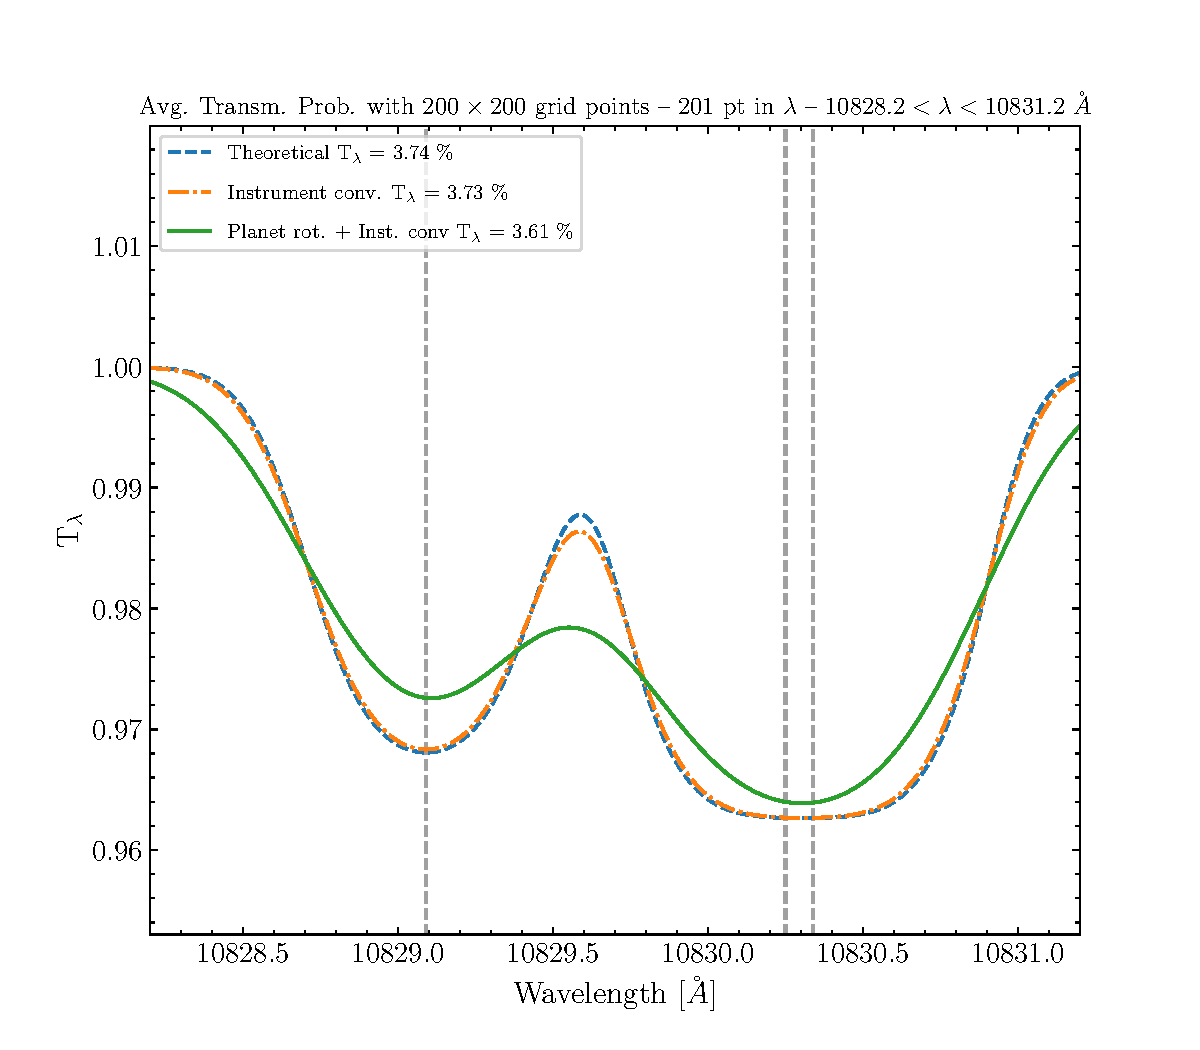
\includegraphics[width=0.49\textwidth]{figures/tpm_He10830.pdf}\hfill
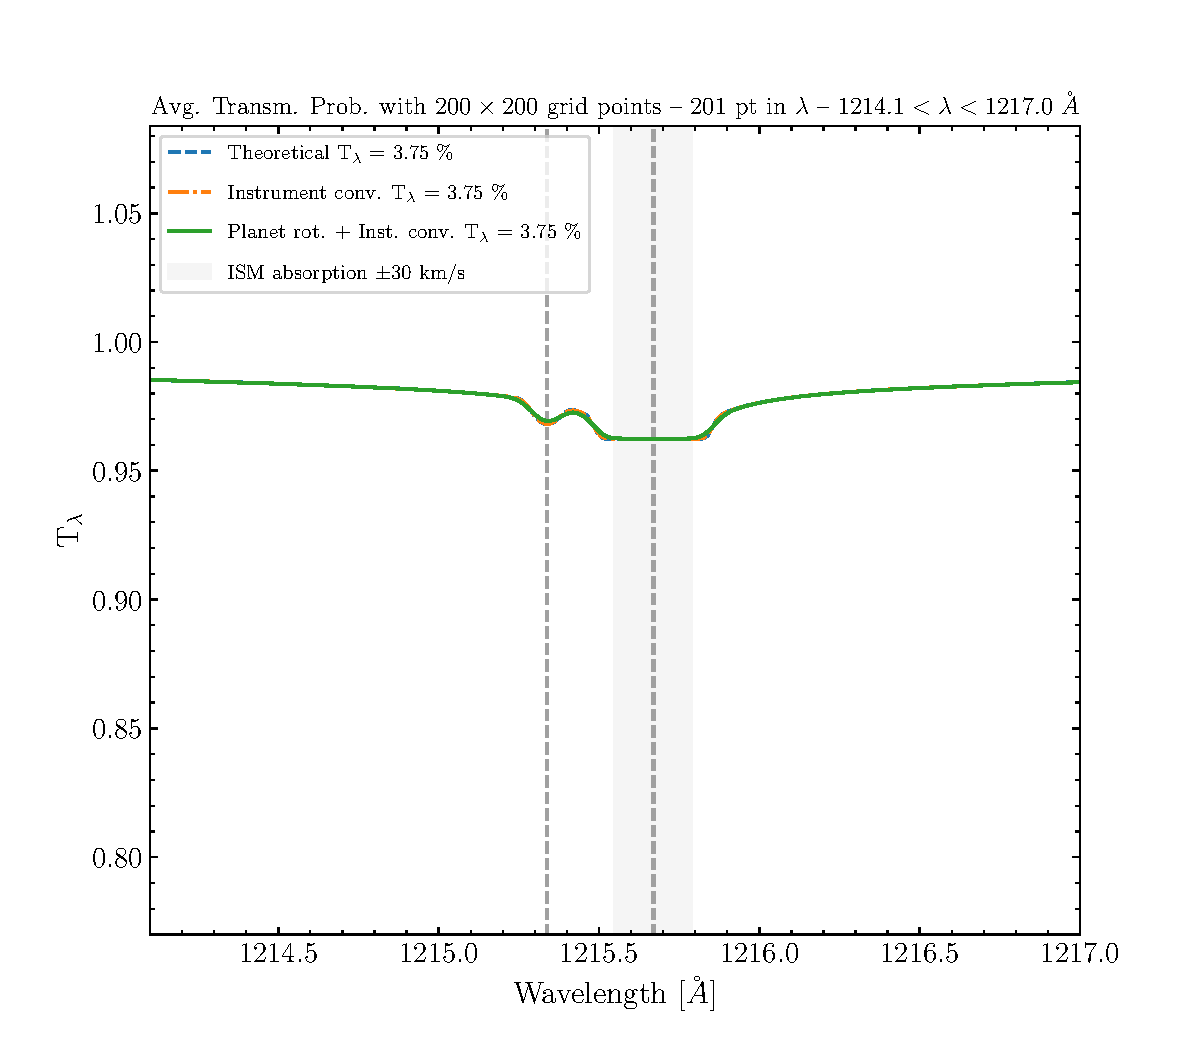
\includegraphics[width=0.49\textwidth]{figures/tpm_Lya.pdf}\\[2pt]
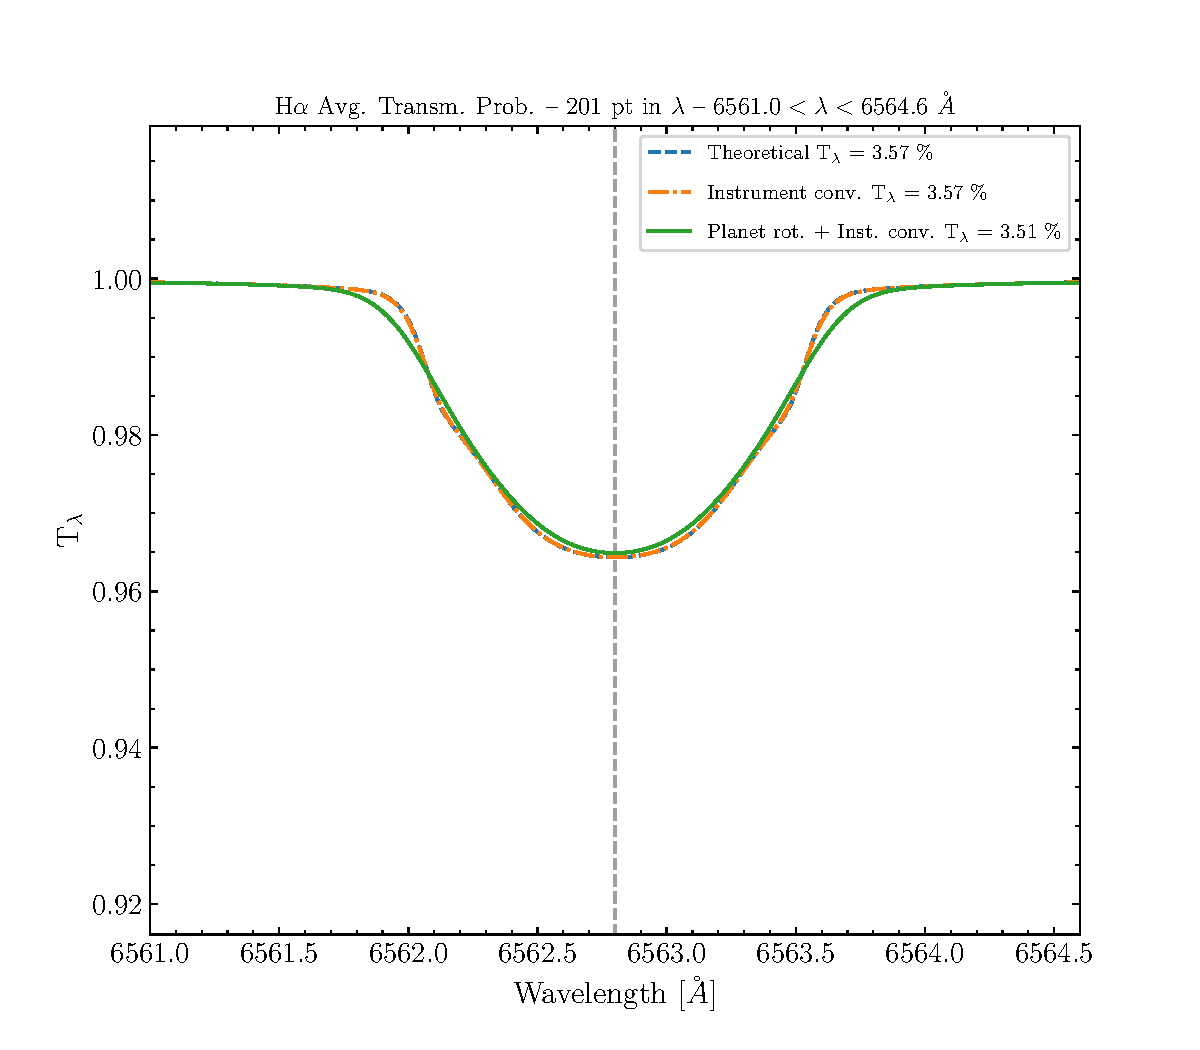
\includegraphics[width=0.49\textwidth]{figures/tpm_Halpha.pdf}\hfill
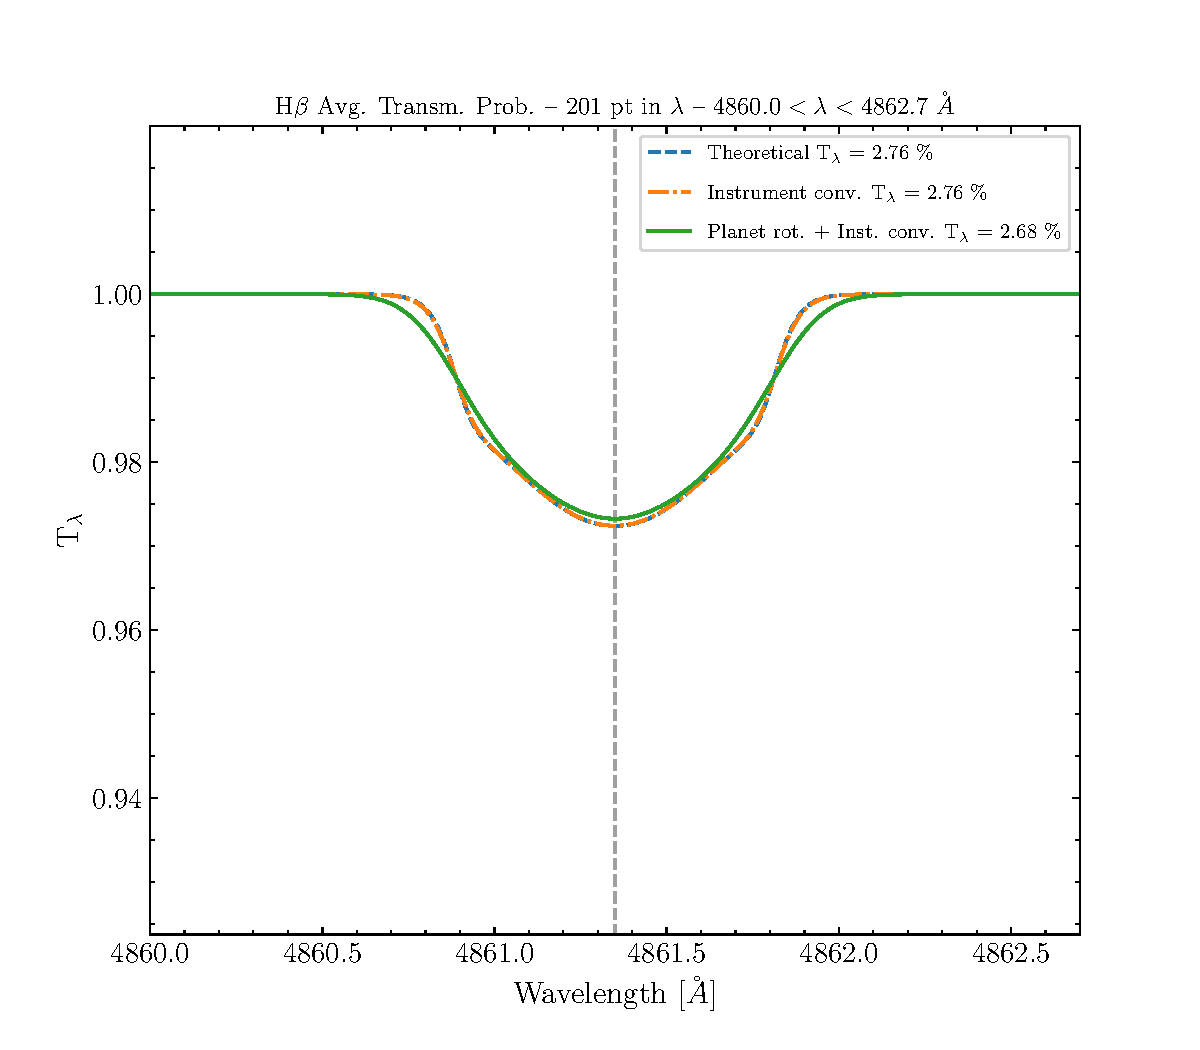
\includegraphics[width=0.49\textwidth]{figures/tpm_Hbeta.pdf}
\caption{\texttt{EXHALE\_transit.py} output spectra for WASP-121b (Roche, Newton solution
with He\,$2^3$S on; \texttt{backup/regression/tpm\_wasp/}): He\,I\,10830 (top left),
Ly$\alpha$ (top right), H$\alpha$ (bottom left), and H$\beta$ (bottom right).
Each panel shows the theoretical line, the instrument-convolved line, and the
instrument$+$rotation-convolved line as produced by the script.}
\label{fig:tpmspec}
\end{figure}

\paragraph{Transit-depth conventions (important).} Huang et al.\ (2023) quote
transit depths as the \emph{effective transit radius} $R_{\rm eff}/R_\star$, not a
percent absorption; convert from the code's line absorption fraction $h$ via
$R_{\rm eff}/R_\star=\sqrt{(R_p/R_\star)^2+h}$. The metal NUV lines (Mg\,II) are
quoted in a 4\,\AA\ bin, while the optical lines (Ca\,II, H$\alpha$, Na) are
line-center; line-center vs.\ 4\,\AA\ can differ by $\sim3\times$ for an
optically-thick line, so always compare in the same definition.

\subsection{\texttt{exhale\_io.py}: named, physical-unit loaders}
\label{sec:atesio}
\texttt{examples/exhale\_io.py} loads every EXHALE output file into named arrays
in physical units, so analysis code need not remember column orders
(Table~\ref{tab:atesio}). The central object is the \texttt{Run} container:
\texttt{load\_run(outdir, inputfile)} fills it with the hydro profiles
(\texttt{r} [$R_p$], \texttt{n} [cm$^{-3}$], \texttt{v} [cm\,s$^{-1}$] with a
\texttt{v\_kms} shortcut, \texttt{p}, \texttt{T}, \texttt{heat},
\texttt{cool}), the full ion-density dictionary \texttt{run.ion} (the 6 H/He
plus 27 metal stages of \S\ref{sec:outputs}), and the parsed
\texttt{input.inp} in \texttt{run.inp}. By default the \texttt{\_adv}
(advection-corrected) files are read; pass \texttt{adv=False} for the
equilibrium snapshot. Typical use:
\begin{lstlisting}[style=sh]
import exhale_io as aio
run = aio.load_run('output', 'input.inp')     # _adv profiles by default
print(aio.mdot_log10(run))                    # log10 Mdot [g/s], 2D factor incl.
print(aio.mdot_Mp_per_Gyr(run))               # same in M_p/Gyr
xh = run.x_ion(['HI', 'HII'])                 # stage fractions of one element
plt.plot(run.r, run.T)
plt.plot(run.r, xh['HII'])
cool = aio.load_cooling('output/Cooling_breakdown.txt')
plt.semilogy(cool['r'], cool['chan']['FeII']) # one cooling channel
\end{lstlisting}

\begin{table}[htbp]\centering\small
\begin{tabular}{@{}lp{8.6cm}@{}}
\toprule
Function & Returns \\
\midrule
\texttt{load\_run(outdir, inputfile, adv=True)} & a \texttt{Run}: hydro
  profiles $+$ \texttt{run.ion} dict $+$ parsed input. \\
\texttt{Run.x\_ion([stages])} & ionization fractions of one element, e.g.\
  \texttt{x\_ion(['HI','HII'])['HII']} $= n_{\rm HII}/(n_{\rm HI}+n_{\rm HII})$. \\
\texttt{load\_hydro(path)} & one \texttt{Hydro\_ioniz(\_adv).txt} as a dict
  (\texttt{r,n,v,p,T,heat,cool}). \\
\texttt{load\_ions(path)} & \texttt{(r, \{ion: density\})} from
  \texttt{Ion\_species(\_adv).txt} (all 33 stages). \\
\texttt{load\_cooling(path)} & \texttt{r,T,ne,cool\_total} $+$
  \texttt{chan} dict of cooling in each channel (6 H/He channels
  \path{rec/coll_ion/coex_HI/coex_HeI/coex_HeII/brems}, the
  \texttt{H3p} infrared channel, $+$ 27 metal-line channels). \\
\texttt{load\_excited\_H(path)} & \texttt{Excited\_H.txt} as a dict
  (\texttt{n2s, n2p, Jlya, tau\_lya, Sproton, Hpe, \ldots}). \\
\texttt{load\_lyman\_werner(path)} & \texttt{Lyman\_Werner.txt} as a dict
  (\texttt{x\_H2, NH2, f\_shield, k\_LW, heat\_LW}). \\
\texttt{read\_input(path)} & \texttt{input.inp} as a dict
  (\texttt{Rp\_RJ, Mp\_MJ, a\_AU, HeH, LX, LEUV, \ldots} $+$ raw lines). \\
\texttt{mdot\_log10(run, j\_from\_top=20)} & $\log_{10}\dot M$ [g/s]:
  $4\pi\rho v r^2$ near the outer boundary \emph{including} the
  \texttt{2D approximate method} factor (mirrors \texttt{EXHALE\_main.f90};
  see \S\ref{sec:outputs}). \\
\texttt{mdot\_Mp\_per\_Gyr(run)} & the same in units of $M_p$\,Gyr$^{-1}$. \\
constants & \texttt{RJ\_CM} (and its alias \texttt{RJ}), \texttt{MJ},
  \texttt{Msun}, \texttt{AU}, \texttt{mu} ($=m_{\rm H}$), \texttt{GYR} (cgs).
  These are the one Python definition of each; the tools import them from here
  rather than writing the number down again. \\
\bottomrule
\end{tabular}
\caption{\texttt{examples/exhale\_io.py} public interface. Run analysis scripts
either from \texttt{examples/} or after adding it to the Python path
(\texttt{sys.path.insert(0, '<repo>/examples')}).}
\label{tab:atesio}
\end{table}

The notebook \texttt{examples/}\allowbreak\texttt{EXHALE\_analysis.ipynb}
uses these loaders to plot the profiles and the parameter-difference
comparisons of \S\ref{sec:examples}, and
\texttt{examples/make\_figures.py} (which generates every figure in this
manual) is a further worked example.

\subsection{\texttt{exhale\_to\_lart.py}: LaRT Ly$\alpha$ input from an EXHALE
run}\label{sec:exhale2lart}
\texttt{EXHALE\_transit.py} estimates the Ly$\alpha$ mean intensity $\bar J_{\rm Ly\alpha}$ with
the simple Huang et al.\ (2017) prescription (\S\ref{sec:excitedH}). For a proper
treatment of the resonant Ly$\alpha$ radiative transfer that sets the $n{=}2$
hydrogen population (and hence H$\alpha$), the converged atmosphere can be
post-processed with the Monte Carlo code \textbf{LaRT} (Seon \& Kim 2020; Seon et
al.\ 2022). \texttt{examples/exhale\_to\_lart.py} builds a complete LaRT
spherical-illumination input set directly from an EXHALE run.

Given a run directory it loads the \texttt{\_adv} profiles (via
\texttt{exhale\_io.py}; \texttt{-{}-eq} takes the equilibrium pair instead,
which is what a stationary solve leaves) and \texttt{input.inp}, and writes
\begin{itemize}\setlength{\itemsep}{0pt}
  \item \texttt{dens\_profile.txt}: $r\,[\Rp]$, $n_{\rm HI}\,[\mathrm{cm^{-3}}]$
        (the Ly$\alpha$ scatterer is ground-state H);
  \item \texttt{temp\_profile.txt}: $r\,[\Rp]$, $T\,[\mathrm{K}]$;
  \item \texttt{velo\_profile.txt}: $r\,[\Rp]$, $v_r\,[\mathrm{km\,s^{-1}}]$;
  \item \texttt{line\_profile.txt}: the incident stellar Ly$\alpha$ profile, a
        double-Gaussian with peaks at $\pm m$ and Gaussian width $s$ (defaults
        $m=74$, $s=49\,\mathrm{km\,s^{-1}}$, the Huang et al.\ 2017 / Yan et al.\
        2022 values; pass \texttt{-{}-fwhm} to read $s$ as FWHM);
  \item \path{<name>_lya.in}: the LaRT namelist
        (\path{geometry='spherical_atmosphere'},
        \path{source_geometry='stellar_illumination'});
  \item \texttt{run.sh}: a multi-host \texttt{mpirun} launcher.
\end{itemize}
The length unit is set to $\Rp$ (\texttt{distance2cm}\,$=R_{\rm p}$ in cm), so all
LaRT radii are in $\Rp$ and match the EXHALE grid; the star--planet geometry
(\texttt{distance\_star\_to\_planet}\,$=a/\Rp$,
\texttt{stellar\_radius}\,$=R_\star/\Rp$) is read from \texttt{input.inp}. Because
the stellar illumination breaks spherical symmetry, the scattering rate is requested
as a cylindrical 2-D grid (\texttt{geometry\_JPa = 2}): $P_\alpha(\rho,z)$ is
axisymmetric about the star--planet axis, which is the form needed to build the 2-D
$n_{2p}(\rho,z)$ population for the H$\alpha$ transit. To populate $P_\alpha$, build
LaRT with \texttt{make CALCPnew=1} (producing \texttt{LaRT\_calcP.x}).

\begin{lstlisting}[style=sh]
# build the LaRT input from a converged EXHALE run, then run it
python examples/exhale_to_lart.py WASP-52b/fxuv0p25_he98 \
       -o WASP-52b/LaRT_lya --name WASP-52b \
       --m 74 --s 49 --rmax 10 --ngrid 201 --nphotons 1e7 \
       --hosts lart4,lart3,lart2
cd WASP-52b/LaRT_lya && ./run.sh
\end{lstlisting}
It is also importable: \texttt{import exhale\_to\_lart as e2l;
e2l.build(run\_dir, outdir, m\_kms=74, s\_kms=49, geometry\_jpa=2, \dots)}.

% ===================================================================== %
\section{Worked examples}\label{sec:examples}
% ===================================================================== %

\subsection{A first run: a generic hot Jupiter}
The directory \texttt{examples/tutorial/} contains a minimal, self-contained
model of a generic HD\,209458b-like hot Jupiter: a spherical domain out to
$10\,R_p$, solar metals, EUV+X-ray power-law SED. The full \texttt{input.inp} is:
\begin{lstlisting}[style=cfg]
Planet name: demoHJ
Log10 lower boundary number density [cm^-3]: 12.70
Planet radius [R_J]: 1.38
Planet mass [M_J]: 0.69
Equilibrium temperature [K]: 1320.0
Orbital distance [AU]: 0.047
Escape radius [R_p]: 2.00
He/H number ratio: 0.083
2D approximate method: Rate/2 + Mdot/2
Parent star mass [M_sun]: 1.13
Spectrum type: Power-law
Power-law index: -1.0
Use only EUV? False
[E_low,E_mid,E_high] = [ 13.60 , 123.98 , 1.24e3 ]
Log10 of X-ray luminosity [erg/s]: 27.0
Log10 of EUV luminosity [erg/s]: 29.30
Grid type: Mixed
Numerical flux: HLLC
Reconstruction scheme: PLM+WENO3
Include He23S? True
Load IC? False
Do only PP: False
Force start: False
Domain mode: Spherical
Outer radius [R_p]: 10.0
du_th [PLM,WENO3]: 0.5 1.0e-3
Solver: Newton
Stellar radius [R_sun]: 1.155
\end{lstlisting}
The \texttt{Reconstruction scheme: PLM+WENO3} line enables the two-stage
reconstruction (with the two \texttt{du\_th} values as the PLM and WENO3
thresholds), and the \texttt{Solver: Newton} line adds the steady-state Newton
finish (\S\ref{sec:newton}), so the run converges to the true steady state
without manual restarts. With \texttt{metals.inp} present (solar
abundances, \S\ref{sec:inputs}), run
\texttt{./EXHALE.x} in that directory. Figure~\ref{fig:tut} shows the converged
profiles read back with \texttt{exhale\_io}: the wind heats to $\sim10^4$\,K, the
velocity rises monotonically outward (transonic outflow), and hydrogen ionizes
across a front near $1.2$--$1.4\,R_p$.

\begin{figure}[htbp]\centering
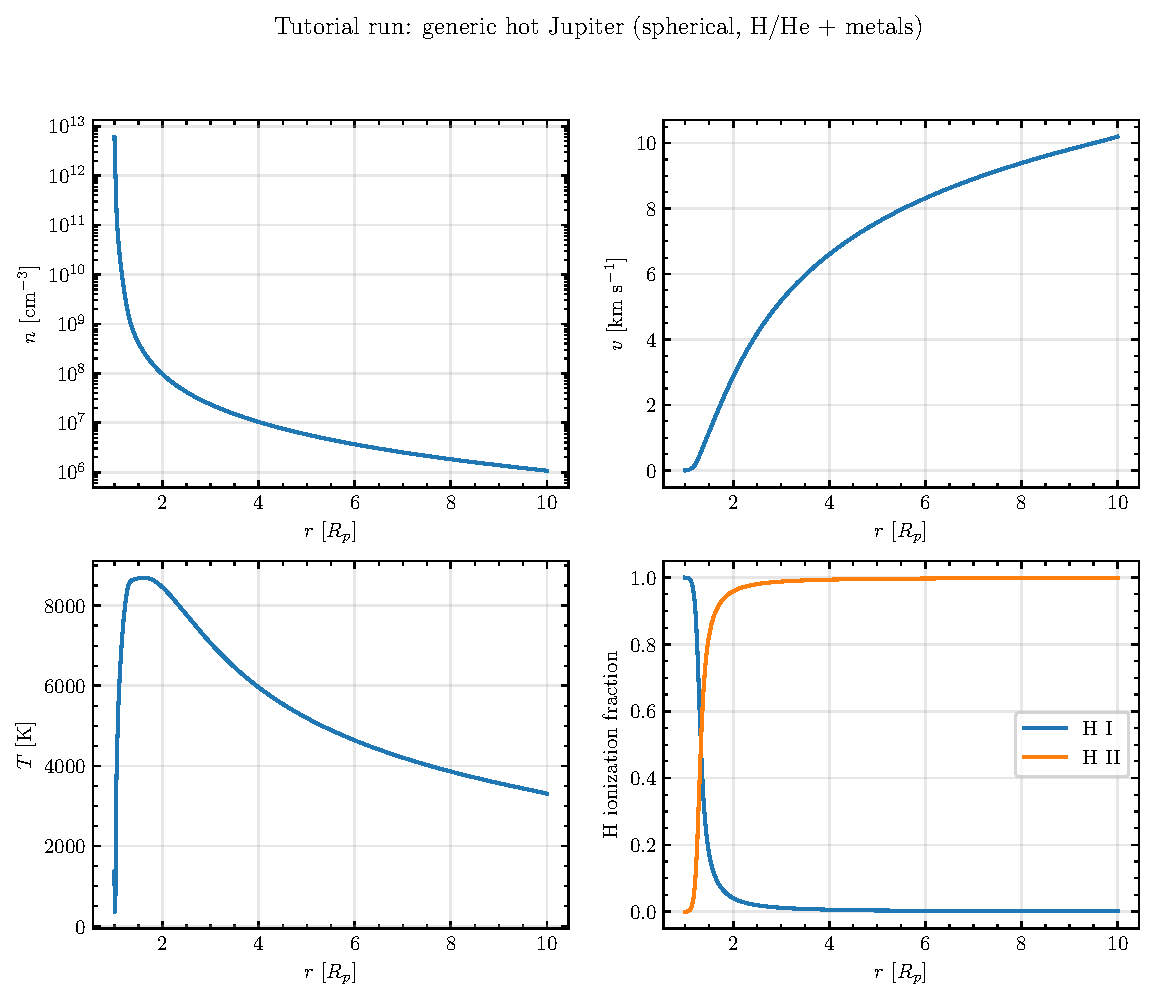
\includegraphics[width=0.92\textwidth]{figures/tutorial_overview.pdf}
\caption{First-run output of the generic hot-Jupiter tutorial: density,
velocity, temperature, and the H ionization fraction vs.\ radius.}
\label{fig:tut}
\end{figure}

\subsection{Turning physics on and off}
The same model is re-run with single-line changes to illustrate each option:
\emph{metals off} by removing \texttt{metals.inp}; \emph{Roche/RLOF} by removing
the \texttt{Domain mode}/\texttt{Outer radius} lines (the default truncates at
L1); the \emph{atomic-helium limit} by setting \texttt{Include He23S? False}
(the triplet is on by default, so this is the change that removes it); the
\emph{H$\alpha$/Balmer} physics by adding \texttt{Stellar Teff}/\texttt{Stellar
radius}; and the \emph{transonic IC} by adding \texttt{Transonic IC: True} for a
near-unbound (deep-RLOF) base; and \emph{diffusive He/H separation} by adding
\texttt{He\_diffusion: True} (extend it to the metals with
\texttt{He\_metal\_diffusion: True}; \S\ref{sec:hediff}). The comparison studies
below quantify the effect of the first two.

\subsection{Ready-made example configurations (\texttt{examples/})}
\label{sec:exinputs}
For every solver/physics combination there is a ready-to-run folder under
\texttt{examples/} (paths relative to the \texttt{EXHALE} root). Folders
\texttt{01}--\texttt{11} are the \emph{same} planet (HD189733b) so that the
effect of each option can be isolated; \texttt{12} and
\texttt{14}--\texttt{17} use HD209458b (where the Wind-AE warm start,
diffusion, molecular chemistry with and without metals, and the
lower-atmosphere profile handoff are validated),
and \texttt{13} spans four planets. Each folder is
self-contained: \texttt{cd} into it and run the repo-root binary
(\texttt{../../EXHALE.x}); outputs land in the folder's own \texttt{output/}.
The ``Added / changed lines'' column of Table~\ref{tab:exinputs} is relative
to each example's natural base: the legacy
\texttt{01\_legacy\_marching/input.inp} for the solver examples
\texttt{02}--\texttt{04} (and Wind-AE \texttt{11}/\texttt{12}), and the
recommended-solver \texttt{03\_newton/input.inp} (two-stage
\texttt{PLM+WENO3}\,$+$\,\texttt{Solver: Newton}) for the physics examples
\texttt{05}--\texttt{10}, which all inherit that solver and add only their
signature option on top. A \texttt{diff} against the appropriate base shows
exactly what an option adds; all configurations have been smoke-tested.
The metastable helium triplet is on by default in the code, but the ladder
holds \texttt{Include He23S? False} on purpose: in both bases and in every
rung whose signature option is something else (\texttt{02}, \texttt{04},
\texttt{05}, \texttt{09}--\texttt{12}), so that atomic helium is the
baseline and \texttt{06\_he23s} remains a one-line difference. Outside the
ladder (\texttt{tutorial/}, \texttt{13}--\texttt{16}, the planet folders) the
triplet is on.
\texttt{11\_windae\_ic} (HD189733b) exercises the self-consistent-BC
continuation: its Wind-AE ramp converges and writes the IC, though EXHALE's own
time-integration of HD189733b is limited by a separate base-breathing
instability (\S\ref{sec:windae}). \texttt{12\_windae\_ic\_hd209} is the
seed-adjacent HD209458b case. \texttt{14\_diffusion} and \texttt{15\_molecular}
turn on the He/metal diffusive separation (\S\ref{sec:hediff}) and the full
molecular network (\S\ref{sec:loweratm}) respectively, on HD209458b, and
\texttt{16\_molecular\_metals} adds a \texttt{metals.inp} to the latter. \texttt{17\_lower\_profile} replaces the scalar
\texttt{base.inp} handoff by the profile of \S\ref{sec:lowerprofile}.

{\small
\begin{longtable}{@{}lp{4.6cm}p{5.6cm}@{}}
\caption{Ready-made example configurations under \texttt{examples/}
(\texttt{01}--\texttt{11} are HD189733b; \texttt{12}, \texttt{14}--\texttt{17}
are HD209458b; \texttt{13} spans four planets). The Wind-AE IC ramp converges
for both of the planets that use it (HD\,189733\,b (\texttt{11}) and
HD\,209458\,b (\texttt{12})), and \texttt{11}, being far from the seed,
additionally exercises the self-consistent-BC continuation and the
molecular-layer turn-off. Metals on/off is a runtime switch: any folder
becomes metals-on by copying a \texttt{metals.inp} into it, molecular folders
included: that is what \texttt{16\_molecular\_metals} is.}
\label{tab:exinputs}\\
\toprule
\texttt{examples/}\ldots & Demonstrates & Added / changed lines \\
\midrule
\endfirsthead
\multicolumn{3}{l}{\small\itshape Table~\ref{tab:exinputs}, continued}\\
\toprule
\texttt{examples/}\ldots & Demonstrates & Added / changed lines \\
\midrule
\endhead
\bottomrule
\endfoot
\texttt{01\_legacy\_marching} & classic ATES~v2 baseline: PLM marching,
  H/He only, Roche domain, $du$-based stop & (none, baseline) \\
\texttt{02\_two\_stage} & two-stage PLM$\to$WENO3 marching
  (\S\ref{sec:convctl}) & \texttt{Reconstruction scheme: PLM+WENO3},
  \texttt{du\_th [PLM,WENO3]: 0.5 1.0e-3} \\
\texttt{03\_newton} & \textbf{recommended default}: two-stage warm-up $+$
  Newton finish (\S\ref{sec:newton}) & $+$ \texttt{Solver: Newton} \\
\texttt{04\_newton\_from\_state} & Newton re-convergence of an existing state
  (no marching; needs \texttt{output/*\_IC.txt}, see the folder
  \texttt{README}) & \texttt{Load IC? True},
  \texttt{Resid tol: 1.0e-5}; run via the \texttt{EXHALE\_PTC} hook \\
\texttt{05\_metals} & trace-metal cooling, solar C/N/O/Mg/Ca/Na/Fe
  (\S\ref{sec:inputs}) & \texttt{metals.inp} present \\
\texttt{06\_he23s} & He~$2^3$S metastable level (He\,I~10830); the one rung
  that leaves the ladder's atomic-helium baseline &
  \texttt{Include He23S? True} \\
\texttt{07\_balmer\_lya} & non-LTE H($n{=}2$) $+$ Ly$\alpha$ pumping
  (H$\alpha$/H$\beta$, \S\ref{sec:jlya}) & $+$ \texttt{Stellar
  Teff/radius}, \texttt{Deexc heat}, \texttt{Jlya escape-prob},
  \texttt{Stellar Lya flux/halfwidth/boost} \\
\texttt{08\_full} & everything on ($=$ the \texttt{HD189733b/} planet folder
  $+$ Newton); feeds \texttt{EXHALE\_transit.py} & \texttt{07} $+$ \texttt{metals.inp} \\
\texttt{09\_spherical} & spherical domain instead of the default Roche/L1
  truncation (\S\ref{sec:potential}) & \texttt{Domain mode: Spherical},
  \texttt{Outer radius [R\_p]: 10.0} \\
\texttt{10\_warm\_seed\_ic} & warm-seed (hot Parker overlay) initial
  condition & \texttt{Hot Parker IC: 10000} \\
\texttt{11\_windae\_ic} & in-process Wind-AE IC for HD189733b
  (\S\ref{sec:windae}): far from the seed, so the self-consistent-BC continuation (base-BC
  re-convergence $+$ molecular-layer turn-off) is exercised; the Wind-AE ramp
  converges and writes the IC. EXHALE's own HD189733b base-breathing
  instability (separate from the IC) then limits the warm start &
  $+$ \texttt{IC mode: windae}, \texttt{Solver: Newton}; symlinks
  \texttt{inputdata/} for the shipped seed \\
\texttt{12\_windae\_ic\_hd209} & in-process Wind-AE warm-start IC that
  \emph{works}: HD\,209458b (\textbf{not} HD189733b) is close to the
  shipped seed, so the ramp converges and EXHALE warm-starts cleanly
  (spherical $10\,R_p$) & HD209458b params $+$ \texttt{Domain mode:
  Spherical}, \texttt{IC mode: windae}, \texttt{Solver: Newton};
  symlinks \texttt{inputdata/} \\
\texttt{13\_lower\_atmosphere} & lower-atmosphere connection for four planets
  (HD209458b, HD189733b, WASP-121b, WASP-52b; \S\ref{sec:loweratm}): an
  analytic $1\,\mu$bar base column plus a \texttt{base.inp} handoff
  (isothermal or Guillot $T(p)$ generator); see the folder \texttt{README} &
  \texttt{Lower column: <R\_1bar>}; driver-generated
  \texttt{base\_iso.inp} / \texttt{base\_guillot.inp} \\
\texttt{14\_diffusion} & diffusive separation of He and metals (HD209458b;
  \S\ref{sec:hediff}): the He/H ratio declines with altitude and each trace
  metal settles independently, reshaping He\,I~10830 & HD209458b params $+$
  \texttt{Include He23S? True}, \texttt{He\_diffusion: True},
  \texttt{He\_metal\_diffusion: True}, \texttt{He\_Kzz: 1.0e9},
  \texttt{He\_alphaT: 0.0}; \texttt{metals.inp} present \\
\texttt{15\_molecular} & full molecular chemistry (HD209458b;
  \S\ref{sec:loweratm}): H$_2$/H$_2^+$/H$_3^+$/HeH$^+$ in the coupled
  ionization equilibrium; a sharp H$_2\!\to$H front forms above a thin
  molecular base, the wind above it essentially atomic. Newton-converged from a
  cold start, re-run 2026-08-15 with the current code ($\|R\| =
  6.105\times10^{-6}$ in 89 outer iterations): the front sits at
  $r=1.0097\,R_p$ and the molecular layer below it collapses to ${\sim}400$\,K &
  HD209458b params $+$ \texttt{Molecular chemistry: True},
  \texttt{Solver: Newton 5.0e-2}, \texttt{Resid tol: 1.0e-7},
  \texttt{Max steps: 150000} (no
  \texttt{metals.inp} here) \\
\texttt{16\_molecular\_metals} & molecular chemistry \emph{and} trace metals
  solved in one system (HD209458b): the H$_2$/H$_2^+$/H$_3^+$/HeH$^+$ network
  and the metal ionization stages share the free electron density, which the
  metals dominate in the shielded molecular base. Converges only from a warm
  restart, and the seed matters: seed it with a \texttt{15} converged by
  \emph{the same binary} (a state left by an older binary is a different seed
  and fails, \texttt{info = 2}), then expect \texttt{info = 0} at
  \texttt{Resid tol: 1.0e-7} and $\log_{10}\dot M = 9.65$--$9.67$. The cold path
  is closed: with metals on, the JFNK line search bottoms near
  $\|R\|\sim10^{-3}$ (worst cell $r=1.021$, momentum) and falls back to
  marching at every \texttt{Low-Mach damping} coefficient tried: off,
  $5\times10^{-3}$, $10^{-2}$, $2\times10^{-2}$ (measured 2026-08-15) &
  as shipped, \texttt{15\_molecular} $+$ \texttt{metals.inp} (solar C/N/O)
  without \texttt{15}'s three convergence keys. For the warm restart put the
  seed run's \texttt{Hydro\_ioniz.txt}/\texttt{Ion\_species.txt} in
  \texttt{output/*\_IC.txt} and use \texttt{15}'s three keys $+$
  \texttt{Load IC?\ True} $+$ \texttt{Low-Mach damping: 5.0e-3} (run
  \texttt{1.0e-2} as well and compare, see the folder \texttt{README}) \\
\texttt{17\_lower\_profile} & lower-atmosphere \emph{profile} handoff
(HD209458b; \S\ref{sec:lowerprofile}): the lower atmosphere handed over as a
table over an interval of pressure instead of the scalars of
\texttt{base.inp}. The base state ($T_0$, $R_0$, $p_{\rm base}$,
$q_{\rm H_2}$), the elemental reservoirs (He/H and solar C/N/O) and
$K_{zz}(r)$ all come from the one file; \texttt{make\_example\_profile.py}
regenerates it & \texttt{14\_diffusion} $+$ \texttt{Lower atmosphere
profile: lower\_atmosphere\_profile.dat}, \emph{minus} \texttt{He\_Kzz}
(the profile carries $K_{zz}$) and \emph{minus} \texttt{metals.inp}
(the profile carries C/N/O) \\
\end{longtable}}

% ===================================================================== %
\section{Comparison studies}\label{sec:compare}
% ===================================================================== %

\subsection{Effect of metal-line cooling (metals on vs.\ off)}
Trace metals add strong line cooling (and some photoionization heating and free
electrons). Figure~\ref{fig:metals} compares the tutorial planet with and without
\texttt{metals.inp}: metal-line cooling lowers the peak temperature by
$\sim1800$\,K (acting as a thermostat that prevents the H/He-only over-heating),
while the H ionization structure is barely changed. The effect is far stronger
for hotter, more irradiated planets (e.g.\ WASP-121b, where metal cooling is
essential to match the observed temperatures); the detailed cooling by channel
budget is in Figure~\ref{fig:cool}.

\begin{figure}[htbp]\centering
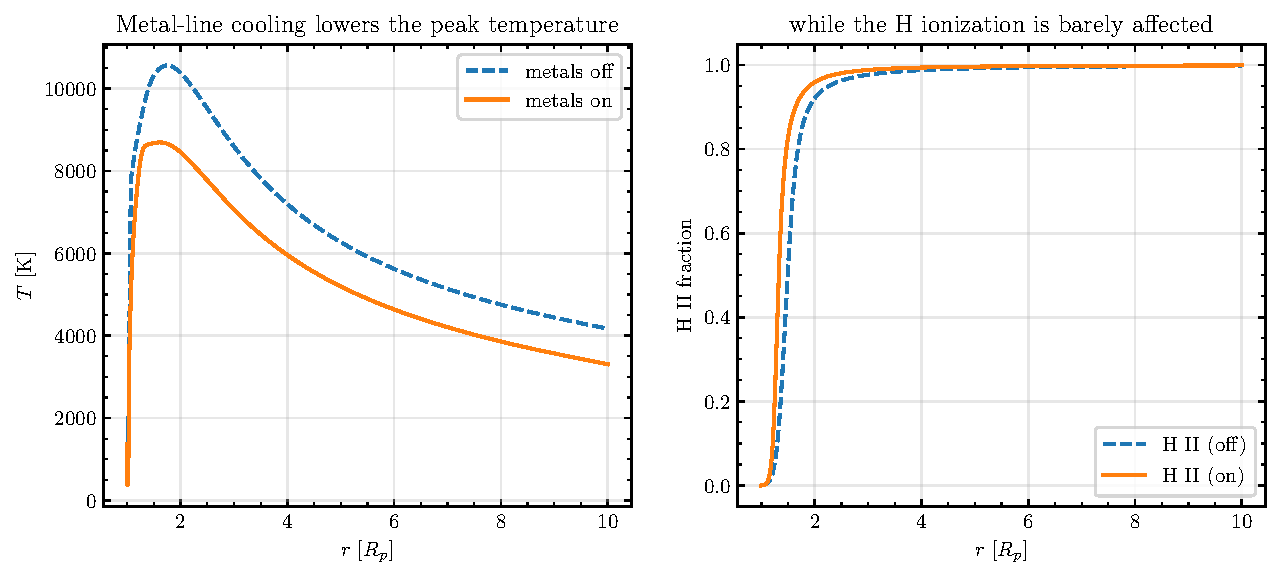
\includegraphics[width=0.95\textwidth]{figures/metals_on_off.pdf}
\caption{Metals on vs.\ off for the tutorial planet: metal-line cooling lowers
the peak temperature (left) while the H ionization fraction is nearly unchanged
(right).}\label{fig:metals}
\end{figure}

\begin{figure}[htbp]\centering
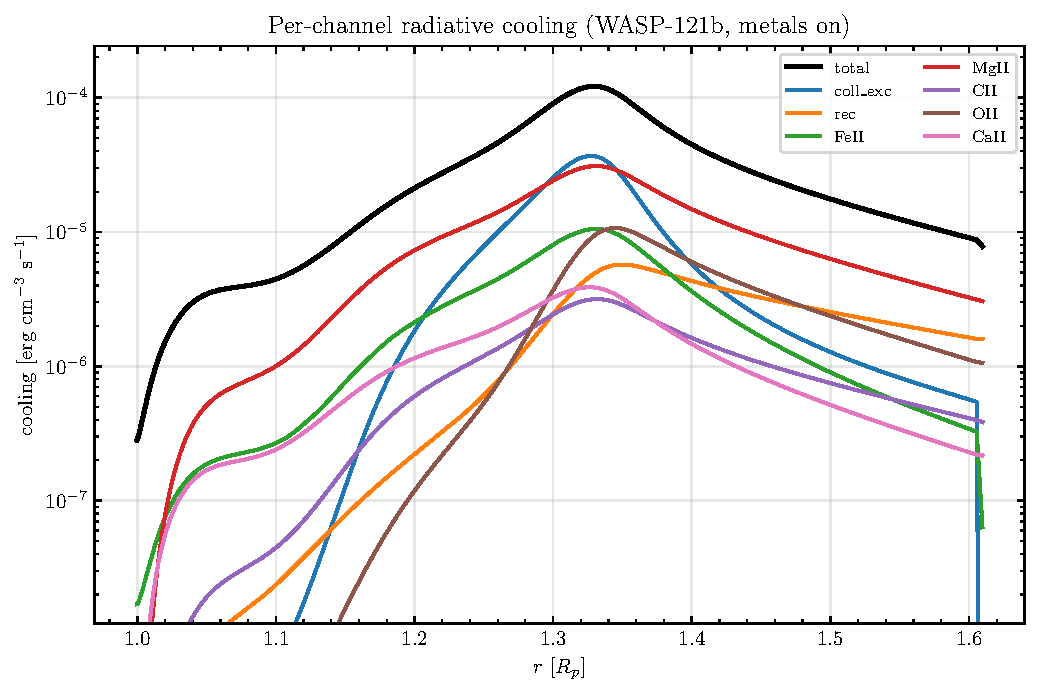
\includegraphics[width=0.72\textwidth]{figures/cooling_breakdown.pdf}
\caption{Radiative cooling by channel vs.\ radius (WASP-121b, metals on; from
\texttt{Cooling\_breakdown.txt}). Below $\sim1.4\,R_p$ the metal lines (e.g.\
Fe\,II, Mg\,II, C/O) compete with or dominate the H/He collisional channels.}
\label{fig:cool}
\end{figure}

\subsection{Spherical vs.\ Roche (RLOF) and the mass-loss rate}
Removing the \texttt{Domain mode: Spherical} line switches on the full Roche
tidal potential, truncated at the L1 radius. Figure~\ref{fig:roche} compares a
spherical model (Case~A) and a Roche model (Case~B) of WASP-121b: the tidal
potential lowers the effective gravity toward the star, so the Roche wind
accelerates far faster and the mass-loss rate rises by an order of magnitude
($\dot M$ from $\sim0.05$ to $\sim0.34\,M_p$\,Gyr$^{-1}$ here), the
``Roche-lobe overflow'' enhancement.

\begin{figure}[htbp]\centering
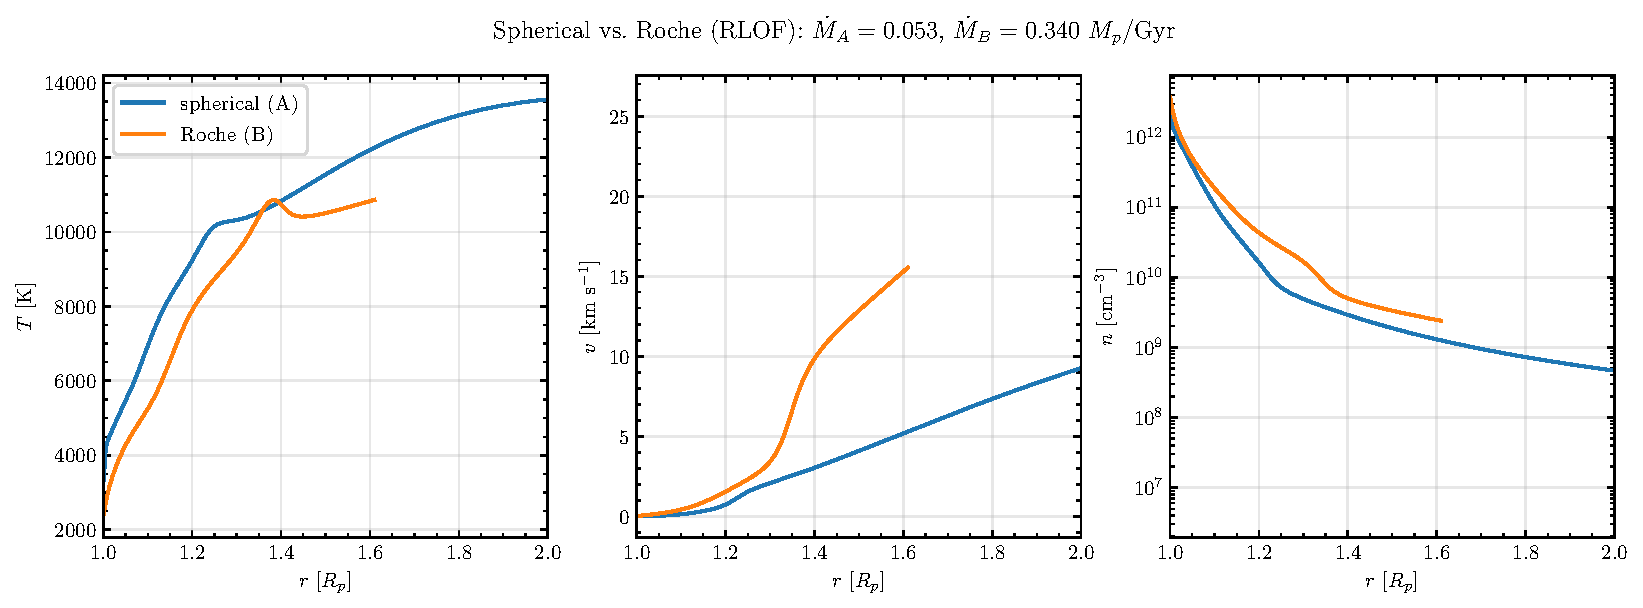
\includegraphics[width=0.98\textwidth]{figures/spherical_vs_roche.pdf}
\caption{Spherical (Case~A) vs.\ Roche (Case~B) WASP-121b: temperature,
velocity, and density. The Roche wind reaches L1 ($\approx1.6\,R_p$) and
accelerates much faster; $\dot M$ is annotated. The temperature panel is the
\texttt{\_adv} profile; its base is smooth because the post-processor falls back
to the equilibrium solution where the flow is not a clean outflow (see the caveat
in \S\ref{sec:outputs}). The Roche velocity (middle) dips slightly negative near
the base: the genuine, physical ``breathing'' inflow of a near-Roche-filling
planet.}\label{fig:roche}
\end{figure}

\subsection{Transmission spectra}
\texttt{EXHALE\_transit.py} turns a converged model into transit absorption. The metal
resonance lines are the key NUV/optical diagnostics; Figure~\ref{fig:trans}
compares the modeled effective transit radii $R_{\rm eff}/R_\star$ (spherical
Case~A) against Huang et al.\ (2023). Recall the conventions of \S5.2: Mg\,II is a
4\,\AA\ bin, Ca\,II/Na are line-center, and $R_{\rm eff}/R_\star=\sqrt{(R_p/R_\star)^2+h}$.

\begin{figure}[htbp]\centering
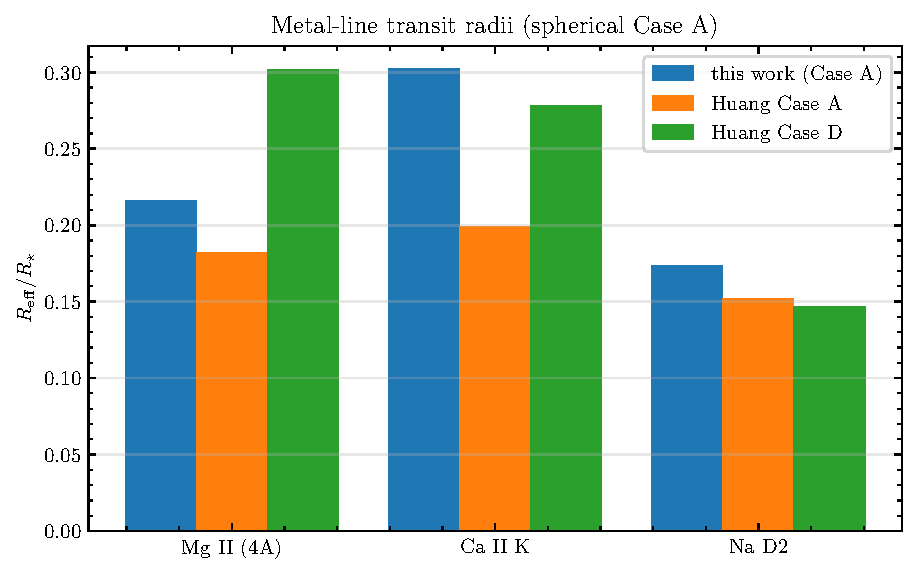
\includegraphics[width=0.66\textwidth]{figures/transmission_metals.pdf}
\caption{Metal-line transit radii $R_{\rm eff}/R_\star$ for spherical Case~A,
compared with Huang et al.\ (2023) Case~A and Case~D.}\label{fig:trans}
\end{figure}

% ===================================================================== %
\section{Atomic and molecular data}\label{sec:data}
% ===================================================================== %
By default EXHALE is an \emph{atomic/ionic} code: the modeled species are H, He
(including the He\,$2\,^3$S metastable triplet), and ten trace metals
(C, N, O, Mg, Si, Ca, Na, K, S, Fe) across their first two--three ionization
stages. The optional molecular network (\texttt{Molecular chemistry: True},
\S\ref{sec:loweratm}) adds H$_2$, H$_2^+$, H$_3^+$ and HeH$^+$ to the coupled
equilibrium, with H$_2$ photoionization opacity (Yan et al.\ 1998) and H$_3^+$
infrared cooling (Miller et al.\ 2013). Beyond those four there is \textbf{no
molecular chemistry and no molecular opacity} (no H$^-$, CO, or H$_2$O),
so no molecular line lists or partition functions enter the calculation.
Table~\ref{tab:data}
collects the provenance of every rate and cross section, grouped by physical
process. The H/He baseline is inherited essentially unchanged from the original
ATES (Caldiroli et al.\ 2021, 2022); the metal, excited-hydrogen, and
charge-exchange data were added in this work.

\begin{longtable}{@{}>{\raggedright\arraybackslash\hyphenpenalty=10000\exhyphenpenalty=10000}p{0.205\textwidth}p{0.30\textwidth}p{0.43\textwidth}@{}}
\caption{Atomic data sources, by process. Source files:
\texttt{cross\_sec.f90} (cross sections); \texttt{Cool\_coeff.f90} (collisional
rates, recombination, cooling); \texttt{charge\_exchange.f90};
\texttt{excited\_hydrogen.f90}; \texttt{EXHALE\_transit.py} (transmission line
data).}\label{tab:data}\\
\toprule
\textbf{Process} & \textbf{Species} & \textbf{Source} \\
\midrule
\endfirsthead
\multicolumn{3}{l}{\small\itshape Table~\ref{tab:data}, continued}\\
\toprule \textbf{Process} & \textbf{Species} & \textbf{Source} \\ \midrule
\endhead
\bottomrule
\endfoot
\multicolumn{3}{@{}l}{\textbf{Elemental abundances}}\\[2pt]
Solar reference & 10 metals (\texttt{metals.inp} template) & Asplund et al.\ (2009) \\
Helium & He/H ratio & input parameter (\texttt{He/H number ratio}) \\
\midrule
\multicolumn{3}{@{}l}{\textbf{Photoionization cross sections}}\\[2pt]
Bound--free $\sigma(E)$ & H\,I & hydrogenic (Kramers) analytic form (orig.\ ATES) \\
 & He\,I & Verner, Ferland, Korista \& Yakovlev (1996) default; legacy ATES 2-term fit via \texttt{ATES\_photoionization\_rate} \\
 & He\,I\,$2\,^3$S (metastable) & two VFKY96 (Verner) wings $+$ power-law bridge, fitted to TOPbase/Opacity-Project (extends the orig.\ Norcross 1971 broken power law past 60\,eV) \\
 & C, N, O, Mg, Si, Na, Fe (+ ions) & Verner, Ferland, Korista \& Yakovlev (1996), single-shell fits \\
 & K\,I & Verner \& Yakovlev (1995) \\
Opacity model (runtime) & all (via \texttt{opacity.inp}) & A=analytic above (default); C=constant above threshold, $\sigma =$ \texttt{OPA\_CONST\_}$X$ times the analytic value at the edge; P=that constant base times the pressure-broadening factor (Robinson \& Catling); T=tabulated files \\
\midrule
\multicolumn{3}{@{}l}{\textbf{Collisional (electron-impact) ionization}}\\[2pt]
Rate $C(T)$ & H\,I, He\,I, He\,II & Voronov (1997, ADNDT 65, 1) default; legacy ATES fits (Abel+1997 / Hui \& Gnedin 1997) via \texttt{Legacy\_HHe\_rates} \\
 & C--Fe, all stages & Voronov (1997, ADNDT 65, 1) \\
\midrule
\multicolumn{3}{@{}l}{\textbf{Recombination (radiative RR + dielectronic DR)}}\\[2pt]
Case~B (RR) & H\,II, He\,II, He\,III & Badnell (2023) RR $-$ Mao \& Kaastra (2016) $\alpha_1$ ($+$ Badnell DR for He\,II) default; legacy Hui \& Gnedin (1997) fits via \texttt{Legacy\_HHe\_rates} \\
He rec.\ radiation $\to$ H\,I (def.\ on, \texttt{He\_rec\_coupling}) & He\,II\,$\to$\,He\,I & Draine (2011) on-the-spot $y$/$z$: extra H\,I photoionization $n_{\rm HeII}n_e[z\,\alpha_B+y\,\alpha_1]$ with photoelectron heating, He\,II recombination shifted to $\alpha_B+y\,\alpha_1$; \texttt{False} $=$ pure case B \\
Metastable & He\,II\,$\to2\,^3$S, $1\,^1$S & power-law fits (orig.\ ATES) \\
Penning ionization & He\,$2\,^3$S\,$+$\,H & Taylor et al.\ (2025) temperature-dependent fit (replaces the const.\ $5\times10^{-10}$; always on) \\
 & He\,$2\,^3$S\,$+$\,H$_2$ & fit to Garc\'{i}a Mu\~{n}oz (2025) Table~A.5 (\texttt{penning\_HeI23S\_H2}, valid 500--10\,000\,K): He\,$2\,^3$S\,$+$\,H$_2\to$\,He\,$1\,^1$S\,$+$\,H$_2^+ + e^-$, releasing $4.4$\,eV to the electrons. The minor H\,$+$\,HeH$^+$ associative-ionization branch is not resolved: the full rate goes to the dominant Penning channel. Active only when a molecular run also tracks the triplet \\
RR + DR & C, N, O, Mg, Si, Na, K, S, Ca\,II (+ stages) & Badnell (2006, ApJS 167, 334) RR + Badnell adf48 DR (TAMOC clist\_K) \\
RR only & Ca\,I (Ca\,II$+e$) & Shull \& Van Steenberg (1982); no DR \\
RR + DR & Fe\,I, Fe\,II & Huang et al.\ (2023) analytic fit; the Badnell DR project does not cover these isoelectronic sequences (see the note below the table) \\
\midrule
\multicolumn{3}{@{}l}{\textbf{Charge exchange (charge transfer)}}\\[2pt]
metal\,$+$\,H/H$^+$ (default) & 23 reactions (Group~A) & Huang et al.\ (2023, ApJ 951, 123) Table~4 \\
He\,$+$\,H/H$^+$ (default on, \texttt{He\_H\_charge\_exchange}) & 2 reactions (Group~B) & Koskinen et al.\ (2013) rates via Huang et al.\ (2023) Table~4; applied by dedicated routines in every helium-bearing system, \emph{not} gated by \texttt{cx\_full} \\
full network (\texttt{cx\_full}) & $+$ metal$+$He, metal$+$metal & Huang et al.\ (2023) Table~4 (Groups C/D) \\
\midrule
\multicolumn{3}{@{}l}{\textbf{Radiative cooling}}\\[2pt]
recomb., coll.\ ion./exc., free--free & H, He & Hui \& Gnedin (1997) recomb.\ cooling; Black (1981) collisional; free--free bremsstrahlung with the van Hoof et al.\ (2014) thermal Gaunt factor, weighted by ion net charge \\
H$_3^+$ infrared (molecular runs) & H$_3^+$ & Miller et al.\ (2013) LTE emission per molecule (Table~5 $z(T)$ fits) times their Table~6 non-LTE departure factor $s(T,n_{\rm H_2})$; optically thin. The dominant coolant of a molecular base, where every atomic channel above is exponentially suppressed \\
metal line cooling \mbox{(analytic)} & C\,I/II, N\,I/II, O\,I/II & closed-form fits to CHIANTI v11.0.2 (default); legacy AIOLOS fits via \texttt{cno\_cool 0} (no N cooling) \\
metal line cooling \mbox{(analytic)} & Mg\,I/II, Ca\,II\,H\&K, Na\,I\,D, Fe\,II coronal & closed-form fits to CHIANTI v11.0.2 (Burgess--Tully descaled; 1--3\% accuracy); Na\,I\,D via effective $\bar g\!\approx\!0.2$ \\
metal line cooling \mbox{(tabulated)} & Fe\,I; Fe\,II\,$(T,n_e)$ & NIST $f$-values $+$ Van Regemorter; CHIANTI multilevel statistical equilibrium \\
ground-term fine structure (statistical equilibrium) & C\,I $2p^2\,^3P$, C\,II $2p\,^2P$, N\,II $2p^2\,^3P$, O\,I $2p^4\,^3P$ & the split ground term is solved in exact statistical equilibrium at the local $(n_e, n_{\rm H\,I})$ instead of the low-density coronal limit, which overstates these lines by 2.9--8.3 decades at the base. Electron collision strengths from CHIANTI v11.0.2; H-atom rates from Yan \& Babb (2023) for C\,I/N\,II, Abrahamsson, Krems \& Dalgarno (2007) for O\,I, Barinovs et al.\ (2005) for C\,II. The coronal curve is kept only for the channels leaving the ground term. The complete set: the other coolants have a single ground level, are built from permitted lines (Fe\,I), or already use a statistical-equilibrium table (Fe\,II) \\
line trapping & the eight ground-term fine-structure lines & line-center escape probability from the column above the cell, Hollenbach \& McKee (1979) / de Jong, Boland \& Dalgarno (1980) plane-parallel Doppler form renormalized to $\beta(0)=1$; applied as $A_{ul}\!\to\!\beta A_{ul}$ \emph{inside} the statistical-equilibrium solution, the only placement correct in both the low- and high-density limits. Other lines, including Mg\,II h\&k, are treated as optically thin \\
validity floor of the coronal fits & all CHIANTI-derived coefficients & the coronal part is cut off smoothly below $10^{3}$\,K (the lower end of the fitted range), continuous in value and $dT$-slope and bit-identical above it; only the explicitly solved ground-term fine-structure terms survive below. The roll-off is $\exp(-x^2)$ with $x=(T_{\rm floor}/T-1)/w$ and $w=0.1$ by default, settable as \texttt{Coronal cutoff width:}. With the C/N/O ground-term fine-structure floors saturated no coronal cooling survives below the floor for the guard to remove, and the base-cell balance temperature of all four paper planets is identical over $w = 0.02$--$1.2$. Not applied to the legacy AIOLOS branch (\texttt{cno\_cool 0}) \\
\midrule
\multicolumn{3}{@{}l}{\textbf{Photoelectric heating}}\\[2pt]
secondary ionization (def.\ on, \texttt{Secondary\_ionization}) & H\,I, He\,I, H$_2$ & Shull \& van Steenberg (1985) $f_{\rm ion}(x)$ fits with the Dalgarno, Yan \& Liu (1999) energy dependence, and Dalgarno et al.'s heating fraction $f_{\rm heat}(x,E_0)$, H$_2$ target channel and molecular heat returns; photoelectrons with $E_0>30\,$eV drive secondary H\,I / He\,I / H$_2$ ionizations, heating scaled to $f_{\rm heat}$; the He\,$2^3$S photoelectron feeds the same heating and secondary-source budget \\
\midrule
\multicolumn{3}{@{}l}{\textbf{Excited hydrogen H($n{=}2$) and Ly$\alpha$}}\\[2pt]
$2s/2p$ rate equilibrium & H($n{=}2$) & Christie, Arras \& Li (2013) Table~2 \\
recombination cascade to $n{=}2$ & H & Draine (2011) \\
Ly$\alpha$ pumping field (mode~0) & H & Huang et al.\ (2017) Eq.~6 \\
\midrule
\multicolumn{3}{@{}l}{\textbf{Transmission line data (\texttt{EXHALE\_transit.py})}}\\[2pt]
$\lambda$, $f$-value, $A_{ki}$ & He\,10830, Ly$\alpha$, H$\alpha$, H$\beta$, Mg\,II, Ca\,II\,H\&K, Na\,I\,D & NIST ASD \\
line profile & all & Voigt (Faddeeva, \texttt{scipy.special.wofz}) \\
\end{longtable}

\noindent
\textbf{Note on Fe.} Iron recombination uses the Huang et al.\ (2023) analytic
RR+DR fit while every other metal uses the Badnell tabulation, and this is not a
deferred item: no Badnell fit exists for either stage. Fe\,I is formed by
recombining Fe\,II (Mn-like, 25 electrons) and Fe\,II by Fe\,III (Cr-like, 24),
whereas the Badnell dielectronic-recombination project reaches the phosphorus
isoelectronic sequence (15 electrons) as of its paper~XVI (2022). Ca\,I has the
same problem one sequence lower (K-like, 19 electrons) and likewise keeps a
non-Badnell rate. \textbf{Note on completeness.} The metal grid carries the stages
needed for the XUV-driven ionization balance and the observed NUV/optical lines;
higher stages and additional elements (e.g.\ the full Fe forest, K\,I, Mg\,I)
beyond those tabulated above are not modeled.

\end{document}
